\documentclass[12pt,spanish,fleqn,openany,letterpaper,pagesize]{scrbook}

\usepackage[utf8]{inputenc}
\usepackage[spanish]{babel}%escribir con acentos sin necesidad de comandos \'{} .
\usepackage{fancyhdr}
\usepackage{epsfig}
\usepackage{epic}
\usepackage{eepic}
\usepackage{amsmath}
\usepackage{threeparttable}
\usepackage{amscd}
\usepackage{here}
\usepackage{graphicx}
\usepackage{lscape}
\usepackage{tabularx}
\usepackage{subfigure}
\usepackage{longtable}


\usepackage{rotating} %Para rotar texto, objetos y tablas seite. No se ve en DVI solo en PS. Seite 328 Hundebuch
                        %se usa junto con \rotate, \sidewidestable ....


\renewcommand{\theequation}{\thechapter-\arabic{equation}}
\renewcommand{\thefigure}{\textbf{\thechapter-\arabic{figure}}}
\renewcommand{\thetable}{\textbf{\thechapter-\arabic{table}}}


\pagestyle{fancyplain}%\addtolength{\headwidth}{\marginparwidth}
\textheight22.5cm \topmargin0cm \textwidth16.5cm
\oddsidemargin0.5cm \evensidemargin-0.5cm%
\renewcommand{\chaptermark}[1]{\markboth{\thechapter\; #1}{}}
\renewcommand{\sectionmark}[1]{\markright{\thesection\; #1}}
\lhead[\fancyplain{}{\thepage}]{\fancyplain{}{\rightmark}}
\rhead[\fancyplain{}{\leftmark}]{\fancyplain{}{\thepage}}
\fancyfoot{}
\thispagestyle{fancy}%


\addtolength{\headwidth}{0cm}
\unitlength1mm %Define la unidad LE para Figuras
\mathindent0cm %Define la distancia de las formulas al texto,  fleqn las descentra
\marginparwidth0cm
\parindent0cm %Define la distancia de la primera linea de un parrafo a la margen

%Para tablas,  redefine el backschlash en tablas donde se define la posici\'{o}n del texto en las
%casillas (con \centering \raggedright o \raggedleft)
\newcommand{\PreserveBackslash}[1]{\let\temp=\\#1\let\\=\temp}
\let\PBS=\PreserveBackslash

%Espacio entre lineas
\renewcommand{\baselinestretch}{1.1}

%Neuer Befehl f\"{u}r die Tabelle Eigenschaften der Aktivkohlen
\newcommand{\arr}[1]{\raisebox{1.5ex}[0cm][0cm]{#1}}

%Neue Kommandos
\usepackage{Befehle}
%Inicio del documento. Tener en cuenta que hay archivos auxiliares

\begin{document}
\pagenumbering{roman}
%\newpage
%\setcounter{page}{1}
\begin{center}
\begin{figure}
\centering%

\epsfig{file=HojaTitulo/EscudoUN,scale=1}%
\end{figure}
\thispagestyle{empty} \vspace*{2.0cm} \textbf{\huge
T\'{\i}tulo de la tesis  o trabajo de investigaci\'{o}n}\\[6.0cm]
\Large\textbf{Nombres y apellidos completos del autor}\\[6.0cm]
\small Universidad Nacional de Colombia\\
Facultad, Departamento (Escuela, etc.)\\
Ciudad, Colombia\\
A\~{n}o\\
\end{center}

\newpage{\pagestyle{empty}\cleardoublepage}

\newpage
\begin{center}
\thispagestyle{empty} \vspace*{0cm} \textbf{\huge
T\'{\i}tulo de la tesis  o trabajo de investigaci\'{o}n}\\[3.0cm]
\Large\textbf{Nombres y apellidos completos del autor}\\[3.0cm]
\small Tesis o trabajo de grado presentada(o) como requisito parcial para optar al
t\'{\i}tulo de:\\
\textbf{Indicar el t\'{\i}tulo que se obtendr\'{a}. Por ejemplo, Magister en Ingenier\'{\i}a Qu\'{\i}mica}\\[2.5cm]
Director(a):\\
T\'{\i}tulo (Ph.D., Doctor, Qu\'{\i}mico, etc.) y nombre del director(a)\\[2.0cm]
L\'{\i}nea de Investigaci\'{o}n:\\
Nombrar la l\'{\i}nea de investigaci\'{o}n en la que enmarca la tesis  o trabajo de investigaci\'{o}n\\
Grupo de Investigaci\'{o}n:\\
Nombrar el grupo en caso que sea posible\\[2.5cm]
Universidad Nacional de Colombia\\
Facultad, Departamento (Escuela, etc.)\\
Ciudad, Colombia\\
A\~{n}o\\
\end{center}

\newpage{\pagestyle{empty}\cleardoublepage}

\newpage
\thispagestyle{empty} \textbf{}\normalsize
\\\\\\%
\textbf{(Dedicatoria o un lema)}\\[4.0cm]

\begin{flushright}
\begin{minipage}{8cm}
    \noindent
        \small
        Su uso es opcional y cada autor podr\'{a} determinar la distribuci\'{o}n del texto en la p\'{a}gina, se sugiere esta presentaci\'{o}n. En ella el autor dedica su trabajo en forma especial a personas y/o entidades.\\[1.0cm]\\
        Por ejemplo:\\[1.0cm]
        A mis padres\\[1.0cm]\\
        o\\[1.0cm]
        La preocupaci\'{o}n por el hombre y su destino siempre debe ser el
        inter\'{e}s primordial de todo esfuerzo t\'{e}cnico. Nunca olvides esto
        entre tus diagramas y ecuaciones.\\\\
        Albert Einstein\\
\end{minipage}
\end{flushright}

\newpage{\pagestyle{empty}\cleardoublepage}

\newpage
\thispagestyle{empty} \textbf{}\normalsize
\\\\\\%
\textbf{\LARGE Agradecimientos}
\addcontentsline{toc}{chapter}{\numberline{}Agradecimientos}\\\\
Esta secci\'{o}n es opcional, en ella el autor agradece a las personas o instituciones que colaboraron en la realizaci\'{o}n de la tesis  o trabajo de investigaci\'{o}n. Si se incluye esta secci\'{o}n, deben aparecer los nombres completos, los cargos y su aporte al documento.\\

\newpage{\pagestyle{empty}\cleardoublepage}

\newpage
\textbf{\LARGE Resumen}
\addcontentsline{toc}{chapter}{\numberline{}Resumen}\\\\
El resumen es una presentaci\'{o}n abreviada y precisa (la NTC 1486 de 2008 recomienda revisar la norma ISO 214 de 1976). Se debe usar una extensi\'{o}n m\'{a}xima de 12 renglones. Se recomienda que este resumen sea anal\'{\i}tico, es decir, que sea completo, con informaci\'{o}n cuantitativa y cualitativa, generalmente incluyendo los siguientes aspectos: objetivos, dise\~{n}o, lugar y circunstancias, pacientes (u objetivo del estudio), intervenci\'{o}n, mediciones y principales resultados, y conclusiones. Al final del resumen se deben usar palabras claves tomadas del texto (m\'{\i}nimo 3 y m\'{a}ximo 7 palabras), las cuales permiten la recuperaci\'{o}n de la informaci\'{o}n.\\

\textbf{\small Palabras clave: (m\'{a}ximo 10 palabras, preferiblemente seleccionadas de las listas internacionales que permitan el indizado cruzado)}.\\

A continuaci\'{o}n se presentan algunos ejemplos de tesauros que se pueden consultar para asignar las palabras clave, seg\'{u}n el \'{a}rea tem\'{a}tica:\\

\textbf{Artes}: AAT: Art y Architecture Thesaurus.

\textbf{Ciencias agropecuarias}: 1) Agrovoc: Multilingual Agricultural Thesaurus - F.A.O. y 2)GEMET: General Multilingual Environmental Thesaurus.

\textbf{Ciencias sociales y humanas}: 1) Tesauro de la UNESCO y 2) Population Multilingual Thesaurus.

\textbf{Ciencia y tecnolog\'{\i}a}: 1) Astronomy Thesaurus Index. 2) Life Sciences Thesaurus, 3) Subject Vocabulary, Chemical Abstracts Service y 4) InterWATER: Tesauro de IRC - Centro Internacional de Agua Potable y Saneamiento.

\textbf{Tecnolog\'{\i}as y ciencias m\'{e}dicas}: 1) MeSH: Medical Subject Headings (National Library of Medicine's USA) y 2) DECS: Descriptores en ciencias de la Salud (Biblioteca Regional de Medicina BIREME-OPS).

\textbf{Multidisciplinarias}: 1) LEMB - Listas de Encabezamientos de Materia y 2) LCSH- Library of Congress Subject Headings.\\

Tambi\'{e}n se pueden encontrar listas de temas y palabras claves, consultando las distintas bases de datos disponibles a trav\'{e}s del Portal del Sistema Nacional de Bibliotecas\footnote{ver: www.sinab.unal.edu.co}, en la secci\'{o}n "Recursos bibliogr\'{a}ficos" opci\'{o}n "Bases de datos".\\

\textbf{\LARGE Abstract}\\\\
Es el mismo resumen pero traducido al ingl\'{e}s. Se debe usar una extensi\'{o}n m\'{a}xima de 12 renglones. Al final del Abstract se deben traducir las anteriores palabras claves tomadas del texto (m\'{\i}nimo 3 y m\'{a}ximo 7 palabras), llamadas keywords. Es posible incluir el resumen en otro idioma diferente al espa\~{n}ol o al ingl\'{e}s, si se considera como importante dentro del tema tratado en la investigaci\'{o}n, por ejemplo: un trabajo dedicado a problemas ling\"{u}\'{\i}sticos del mandar\'{\i}n seguramente estar\'{\i}a mejor con un resumen en mandar\'{\i}n.\\[2.0cm]
\textbf{\small Keywords: palabras clave en ingl\'{e}s(m\'{a}ximo 10 palabras, preferiblemente seleccionadas de las listas internacionales que permitan el indizado cruzado)}\\

\renewcommand{\tablename}{\textbf{Tabla}}
\renewcommand{\figurename}{\textbf{Figura}}
\renewcommand{\listtablename}{Lista de Tablas}
\renewcommand{\listfigurename}{Lista de Figuras}
\renewcommand{\contentsname}{Contenido}


%\newcommand{\clearemptydoublepage}{\newpage{\pagestyle{empty}\cleardoublepage}}
\cleardoublepage

\addcontentsline{toc}{chapter}{Lista de figuras} % para que aparezca en el indice de contenidos
\listoffigures % indice de figuras

\cleardoublepage
\addcontentsline{toc}{chapter}{Lista de tablas} % para que aparezca en el indice de contenidos
\listoftables % indice de tablas

%\chapter*{Lista de s\'{\i}mbolos}
\addcontentsline{toc}{chapter}{\numberline{}Lista de s\'{\i}mbolos}
Esta secci\'{o}n es opcional, dado que existen disciplinas que no manejan s\'{\i}mbolos y/o abreviaturas.\\

Se incluyen s\'{\i}mbolos generales (con letras latinas y griegas), sub\'{\i}ndices, super\'{\i}ndices y abreviaturas (incluir s\'{o}lo las clases de s\'{\i}mbolos que se utilicen). Cada una de estas listas debe estar ubicada en orden alfab\'{e}tico de acuerdo con la primera letra del s\'{\i}mbolo.
\section*{S\'{\i}mbolos con letras latinas}
 \label{simbolos}
 \renewcommand{\arraystretch}{1.3}
%\begin{longtable}[l]{*{4}{>{$}l<{$}}p{9cm}}
\begin{longtable}[l]{>{$}l<{$}l>{$}l<{$}>{$}l<{$}}
%\begin{tabular}
\textbf{S\'{\i}mbolo}&\textbf{T\'{e}rmino}&\textbf{Unidad SI}&\textbf{Definici\'{o}n}\\[0.5ex]\hline
\endfirsthead%
\textbf{S\'{\i}mbolo}&\textbf{T\'{e}rmino}&\textbf{Unidad SI}&\textbf{Definici\'{o}n}\\[0.5ex]\hline
\endhead%
      A              &\'{A}rea                                   &\text{m}^{2}                         &\int\int dxdy\\%
      A_{\text{BET}} &\'{A}rea interna del s\'{o}lido                &\frac{\text{m}^{2}}{\text{g}}        &\text{ver DIN ISO 9277}\\%
      A_{\text{g}}   &\'{A}rea transversal de la fase gaseosa    &\text{m}^{2}                         &\text{Ec...}\\%
      A_{\text{s}}   &\'{A}rea transversal de la carga a granel  &\text{m}^{2}                         &\text{Ec...}\\%
      a              &Coeficiente                            &1                                    &\text{Ec...}\\%
      a              &Contenido de ceniza                    &1                                    &\frac{m_{\text{ceniza}}}{m_{\text{bm,0}}}\\%
      c              &Contenido de carbono                   &1                                    &\frac{m_{\text{C}}}{m}\\%
      c              &Longitud de la cuerda                  &\text{m}                             &\text{Figura...}\\
      c              &Concentraci\'{o}n de la cantidad de materia&\frac{\text{mol}}{\text{m}^{3}}      &\frac{n}{V}\\%
      D              &Di\'{a}metro                               &\text{m}                             &\\%
      E_{\text{A}}   &Energ\'{\i}a de activaci\'{o}n                  &\frac{\text{kJ}}{\text{mol}}         &\text{Ec....}\\%
      F              &Fracci\'{o}n de materia vol\'{a}til            &1                                    &\text{ver DIN 51720}\\%
      Fr             &N\'{u}mero de Froude                       &1                                    &\frac{\omega^{2}R}{g_{\text{0}}}\\%
      \overrightarrow{g}&Aceleraci\'{o}n de la gravedad          &\frac{\text{m}}{\text{s}^{2}}        &\frac{d^{2}\overrightarrow{r}}{dt^{2}}\\%
      H              &Entalp\'{\i}a                               &\text{J}                             &U+PV\\%
      H_{\text{o}}   &Poder calor\'{\i}fico superior              &\frac{\text{MJ}}{\text{kg}}          &\text{ver DIN 51857}\\%
      h              &Contenido de hidr\'{o}geno                 &1                                    &\frac{m_{\text{H}}}{m}\\%
      K              &Coeficiente de equilibrio              &1                                    &\text{Ec...}\\%
      L              &Longitud                               &\text{m}                             &DF\\%
      L              &Longitud del reactor                   &\text{m}                             &\text{Figura...}\\%
      m              &Masa                                   &\text{kg}                            &DF\\%
      \dot{m}        &Flujo de masa                          &\frac{\text{kg}}{\text{s}}           &\frac{m}{t}\\%
      n              &Velocidad de rotaci\'{o}n                  &\frac{\text{1}}{\text{s}}            &\frac{\omega}{2\pi}\\%
      n              &Cantidad de materia                    &\text{mol}                           &DF\\%
      P              &Presi\'{o}n                                &\text{Pa}                            &\frac{\vec{F}\cdot\vec{n}}{A}\\%
      Q              &Calor                                  &\text{kJ}                            &\text{1. $LT$}\\%
      T              &Temperatura                            &\text{K}                             &DF\\%
      t              &Tiempo                                 &\text{s}                             &DF\\%
      x_{\text{i}}   &Fracci\'{o}n de la cantidad de materia     &1                                    &\frac{n_{\text{i}}}{n}\\%
      V              &Volumen                                &\text{m}^{3}                         &\int{dr^{3}}\\%
      \vec{u}        &Velocidad                              &\frac{\text{m}}{\text{s}}            &(\frac{dr}{dt},r\frac{d\upsilon}{dt},\frac{dz}{dt})\\%
      w_{\text{i}}   &Fracci\'{o}n en masa del componente i      &1                                    &\frac{m_{\text{i}}}{m_{\text{0}}}\\%
      w_{\text{w,i}} &Contenido de humedad de la sustancia i &1                                    &\frac{m_{\text{\wasser}}}{m_{\text{i,0}}}\\%
      Z              &Factor de gases reales                 &1                                    &\frac{pv}{RT}\\%
\end{longtable}
\vspace{5ex}
\section*{S\'{\i}mbolos con letras griegas}

\begin{longtable}[l]{>{$}l<{$}l>{$}l<{$}>{$}l<{$}}
\textbf{S\'{\i}mbolo}&\textbf{T\'{e}rmino}&\textbf{Unidad SI}&\textbf{Definici\'{o}n}\\[0.5ex] \hline%
\endfirsthead%
\textbf{S\'{\i}mbolo}&\textbf{T\'{e}rmino}&\textbf{Unidad SI}&\textbf{Definici\'{o}n}\\[0.5ex] \hline%
\endhead%
\renewcommand{\arraystretch}{1.3}
 \label{simbolosg}
     \alpha_{\text{BET}}  &Factor de superficie                  &\frac{\text{m}^{2}}{\text{g}}   &(w_{\text{F,waf}})(A_{\text{BET}})\\%
     \beta_{\text{i}}     &Grado de formaci\'{o}n del componente i   &1                               &\frac{m_{\text{i}}}{m_{\text{bm,0}}}\\%
     \gamma               &Wandhaftreibwinkel (Stahlblech)       &1                               &\text{Secci\'{o}n...}\\
     \epsilon             &Porosidad de la part\'{\i}cula             &1                               &1-\frac{\rho_{\text{s}}}{\rho_{\text{w}}}\\%
     \eta                 &mittlere Bettneigungswinkel (St\"{u}rzen) &1                               &\text{Figura...}\\%
     \theta               &\'{A}ngulo de inclinaci\'{o}n de la cama      &1                               &\text{Figura...}\\
     \theta_{\text{O}}    &\'{A}ngulo superior de avalancha          &1                               &\text{Figura...}\\
     \theta_{\text{U}}    &\'{A}ngulo inferior de avalancha          &1                               &\text{Figura...}\\
     \kappa               &Velocidad de calentamientoe           &\frac{\text{K}}{\text{s}}       &\frac{dT}{dt}\\%
     \nu                  &Coeficiente estequiom\'{e}trico           &1                               &\text{ver DIN 13345}\\%
     \rho_{\text{b}}      &Densidad a granel                     &\frac{\text{kg}}{\text{m}^{3}}  &\frac{m_{\text{S}}}{V_{\text{S}}}\;(\text{Secci\'{o}n...})\\
     \rho_{\text{s}}      &Densidad aparente                     &\frac{\text{kg}}{\text{m}^{3}}  &\frac{m_{\text{F}}}{V_{\text{P}}}\;(\text{Secci\'{o}n...})\\
     \rho_{\text{w}}      &Densidad verdadera                    &\frac{\text{kg}}{\text{m}^{3}}  &\frac{m_{\text{F}}}{V_{\text{F}}}\;(\text{Secci\'{o}n...})\\
     \tau                 &Tiempo adimensional                   &1                               &\text{Ec....}\\%
     \Phi_{\text{V}}      &Flujo volum\'{e}trico                     &\frac{\text{m}^{3}}{\text{s}}   &\frac{\Delta V}{\Delta t}\\
     \omega               &Velocidad angular                     &\frac{1}{\text{s}}              &\frac{d\upsilon}{dt}\\

\end{longtable}


\section*{Sub\'{\i}ndices}
\begin{longtable}[l]{>{}l<{}l}
  \textbf{Sub\'{\i}ndice} & \textbf{T\'{e}rmino} \\[0.5ex] \hline%
  \endfirsthead%
  \textbf{Sub\'{\i}ndice} & \textbf{T\'{e}rmino} \\[0.5ex] \hline%
  \endhead%
\renewcommand{\arraystretch}{1.4}\label{simbolosg}

 bm&materia org\'{a}nica\\%
 DR&Dubinin-Radushkevich\\%
 E&Experimental\\%
 g&Fase gaseosa\\%
 k&Condensado\\%
 Ma&Macroporos\\%
 P&Part\'{\i}cula\\%
 p&Poro\\%
 p&Pirolizado\\%
 R&Reacci\'{o}n\\%
 t&Total\\%
 wf&Libre de agua\\%
 waf&Libre de agua y de ceniza\\%
 0&Estado de referencia\\%

\end{longtable}


\setlength{\extrarowheight}{0pt}


\section*{Super\'{\i}ndices}
\begin{longtable}[l]{>{}l<{}l}
  \textbf{Super\'{\i}ndice} & \textbf{T\'{e}rmino} \\[0.5ex] \hline%
  \endfirsthead%
  \textbf{Super\'{\i}ndice} & \textbf{T\'{e}rmino} \\[0.5ex] \hline%
  \endhead%
\renewcommand{\arraystretch}{1.4}\label{simbolosg}

 n &Coeficiente x\\%



\end{longtable}


\setlength{\extrarowheight}{0pt}


\section*{Abreviaturas}
\begin{longtable}[l]{>{}l<{}l}
  \textbf{Abreviatura} & \textbf{T\'{e}rmino} \\[0.5ex] \hline%
  \endfirsthead%
  \textbf{Abreviatura} & \textbf{T\'{e}rmino} \\[0.5ex] \hline%
  \endhead%
\renewcommand{\arraystretch}{1.4}\label{simbolosg}
 1.$LT$&Primera ley de la termodin\'{a}mica\\%
 $DF$    &Dimensi\'{o}n fundamental\\%
 $RFF$   &Racimos de fruta fresca\\%

\end{longtable}


\setlength{\extrarowheight}{0pt}
%\include{Resumen}%\newcommand{\clearemptydoublepage}{\newpage{\pagestyle{empty}\cleardoublepage}}
\pagenumbering{arabic}
\chapter{Introducción}

\subsection{Regiones activas.}
Las regiones activas son zonas en el Sol comparables con el tamaño de la tierra con una fuerte presencia de campo magnético, es decir, un área donde las lineas de campo internas del Sol pueden emerger de la fotósfera creando un bucle con polaridad negativa de un lado y positiva del otro, este particular fenómeno hace que se arrastre plasma de la superficie a zonas más altas en la atmósfera solar causando un cambio de densidad y enfriando el plasma; esto hace que en observaciones en el visible las manchas solares se vean oscuras, dado que su temperatura es levemente menor (4000K) a la de la fotósfera  (5777K).\\
Estas regiones debido a que concentran una gran intensidad de campo magnético confinado son epicentro de eventos muy energéticos como lo son las \textbf{erupciones solares} que ocurren en la cromosfera y las \textbf{eyecciones de masa coronal (CME)} en la corona solar. Estos eventos se generan cuando la concentración de campo es tan fuerte que se genera el fenómeno llamado \textbf{reconexión magnética} en el cual las lineas de campo se cruzan, generando una explosión que arrastra todo el plasma confinado en el bucle, dependiendo de que tan energético sea esta, podrá arrojar material hasta ser desprendido del Sol como es el caso de las CME.\\

Puesto que no se pueden predecir esta clase de eventos, actualmente se estudian con ayuda de satélites y observaciones terrestres en gran parte del espectro electro magnético e incluso en altas energías como los rayos X debido a la fuerte aceleración que pueden sufrir los iones al interior del bucle.



%%%%%%%%%%%--------------------------------------%%%%%%%%%%%%%%%%%%%%%%---------------%%%%%%%%%%%%%%%%%%%%%%%%%%

\subsection{Fibras ópticas.}
Las fibras ópticas son un elemento óptico el cual se basa en un caso especial que experimenta la luz sobre una interfaz que divide dos medios con diferente permitividad eléctrica y permeabilidad magnética llamado \textbf{reflexión total}, dicha reflexión también depende del ángulo entre el frente de onda de la fuente y el vector normal a la interfaz, de esta manera la fibra óptica se comporta como una guía de onda para IR-VIS-UV.\\
Para hacer una mejor descripción del fenómeno suponemos polarización paralela con lo cual se desarrollarán las ecuaciones de continuidad que deben cumplir los campos incidente, reflejado y transmitido al interactuar con la interfaz entre los dos medios, dichas ecuaciones dan resultado a la \textbf{ley de Snell} y a las \textbf{ecuaciones de Fresnel}. 

\begin{figure}[H]
\centering
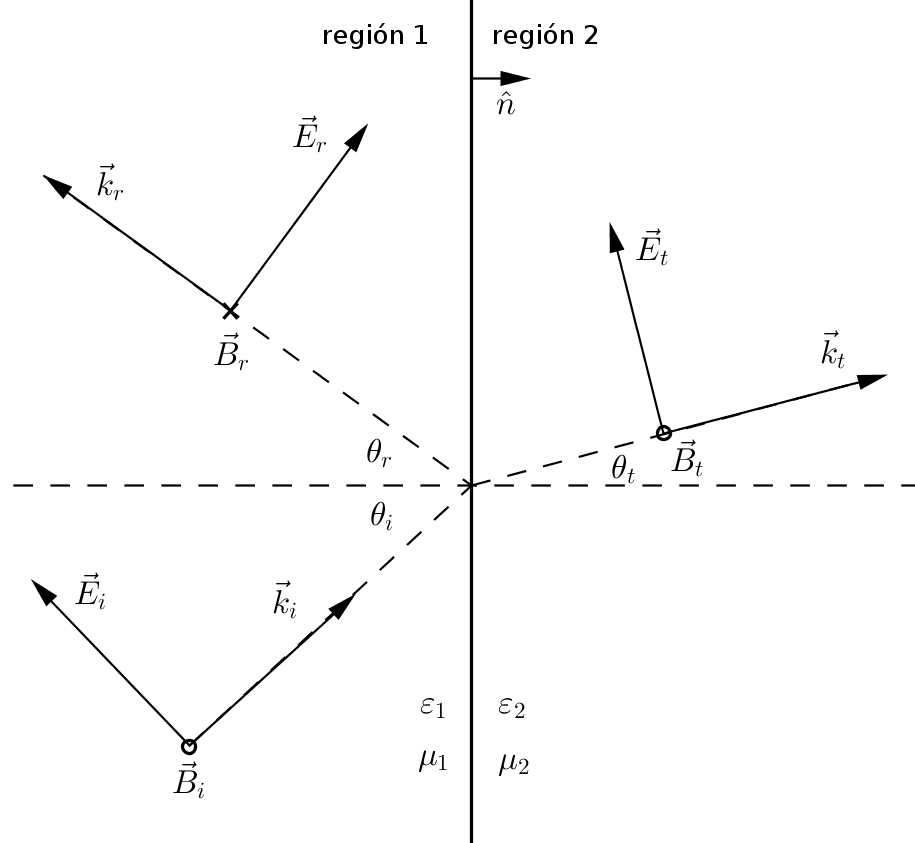
\includegraphics[width=0.46\linewidth]{Kap1/interfaz.png}
\caption{Incidencia oblicua de una onda plana, caso polarización paralela para dos medios con $\varepsilon_1$,$\mu_1$ y $\varepsilon_2$,$\mu_2$ respectivamente.} 
\label{interfaz}
\end{figure}

En la figura \ref{interfaz} se muestra la signatura y orientación escogida para los campos eléctrico y magnético antes y después de interactuar con la interfaz, ya con esto podemos obtener la ley de Snell a partir de la continuidad en las componentes tangenciales, de los campos incluido el vector de onda, es decir las componentes paralelas a la superficie de interfase así como la componente paralela del vector de onda. Esto lo podemos escribir como

\begin{equation}\label{continuidad}
    \hat{n} \times (\Vec{E}_2 - \Vec{E}_1) = 0 \hspace{3mm}\text{ y }\hspace{3mm}\hat{n} \times (\Vec{H}_2 - \Vec{H}_1) = 0
\end{equation}
con lo cual usando (\ref{continuidad}) se obtiene
\begin{equation}\label{continuidad2}
    k_{i,\parallel} = k_{r,\parallel} = k_{t,\parallel} = k_{\parallel} \xrightarrow{} k_{\parallel}=k_i \sin{\theta_i}=k_r \sin{\theta_r}=k_t \sin{\theta_t}.
\end{equation}
Usando la relación de dispersión para cada medio $k=\frac{\omega}{v}=\frac{\omega}{c}\frac{c}{v}=\frac{\omega}{v}n$ donde $n$,$v$ son el índice de refracción y velocidad de la onda en el medio respectivamente, resultando:
\begin{equation}\label{snell}
    n_i\sin{\theta_i}=n_r\sin{\theta_r}=n_t\sin{\theta_t}=cte \hspace{15mm}\text{\textbf{Ley de Snell.}}
\end{equation}
Ahora usando la ecuación (\ref{snell}) imponemos una condición para que el haz sea transmitido al límite de $\theta_t=\pi/2$ despejando tenemos
\begin{equation}\label{total}
    \theta_c = \arcsin{\frac{n_2}{n_1}}
\end{equation}
donde $\theta_c$ es el ángulo mínimo de incidencia con $n_2<n_1$, dicha condición es la que da lugar a la \textbf{reflexión total interna} dado que todo haz que incida con un ángulo mayor tendrá componente netamente reflejada; a éste ángulo lo denominamos \textbf{ángulo crítico}.

\begin{figure}[H]
\centering
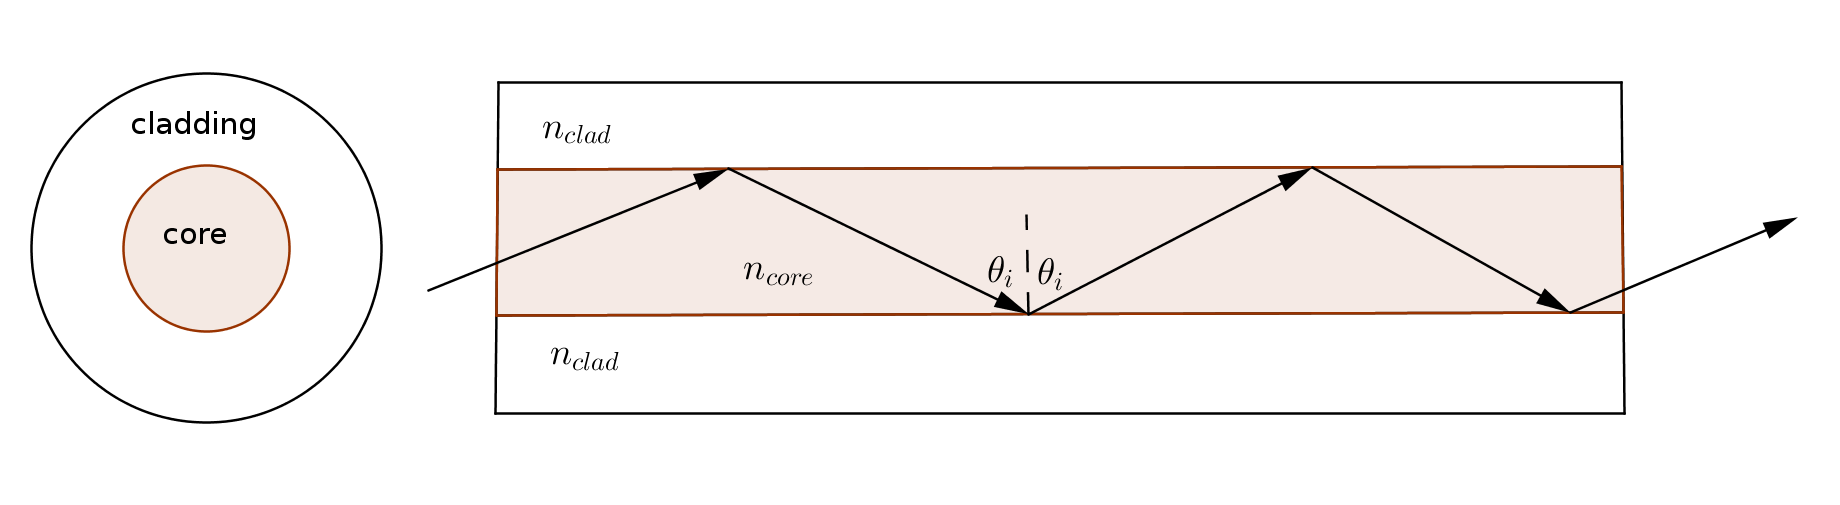
\includegraphics[width=0.76\linewidth]{Kap1/fibra.png}
\caption{Comportamiento de un haz al interior de una fibra óptica.} 
\label{fibra}
\end{figure}
En la figura \ref{fibra} se muestra el esquema de una fibra óptica la cual se compone de dos regiones con diferentes índices de refracción llamados núcleo (core) y revestimiento (cladding) donde $n_{clad}<n_{core}$, así todo haz que cumpla la relación (\ref{total}) se propagará dentro del núcleo, mientras que para ángulos menores los haces serán absorbidos por el revestimiento.


%%%%----------------------------------------------%%%%
%%%%----------------------------------------------%%%%

\subsection{Propiedades ópticas de las fibras.}
Ya entendido el mecanismo de trasporte en una fibra óptica entraremos más en detalle a propiedades importantes de éste elemento óptico como lo son la atenuación de la señal y optimización para diferentes longitudes de onda los cuales dependen en gran parte de los procesos de construcción.\\
Puesto que las propiedades suelen cambiar dependiendo del tipo de construcción se explicarán los tipos de fibras más usuales.

\begin{figure}[H]
\centering
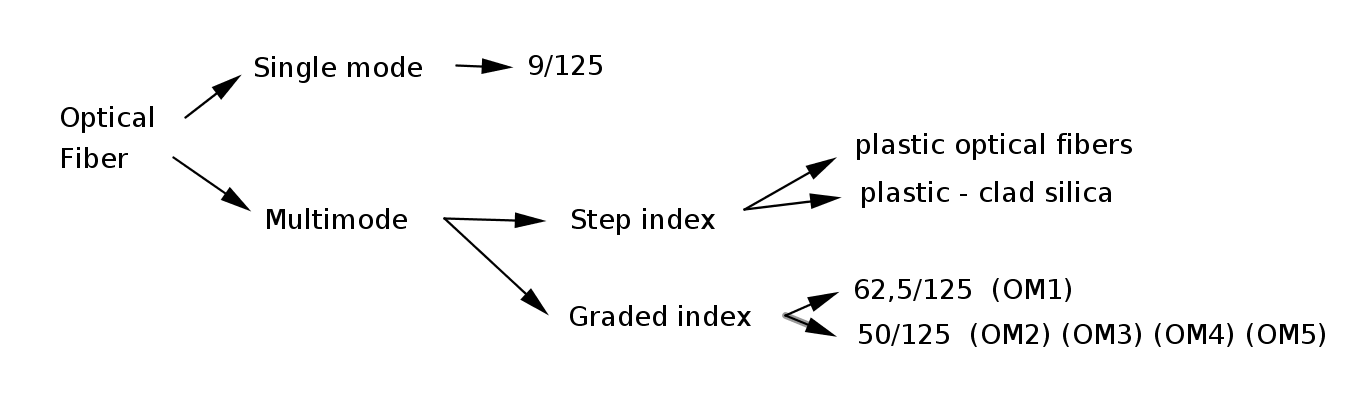
\includegraphics[width=0.76\linewidth]{Kap1/tipos_fibras.png}
\caption{Tipos de fibras ópticas más comunes en el mercado donde se muestran los tamaños de fibras más usados; diámetro núcleo/diámetro revestimiento en $\mu$m.} 
\label{tipos_fibras}
\end{figure}

En la figura \ref{tipos_fibras} se observan las fibras ópticas comúnmente usadas dentro de las cuales resaltan tres grandes grupos, las fibras monomodo , multimodo con salto de índice y multimodo con gradiente de índice. Las fibras monomodo se destacan precisamente por privilegiar un único camino en el cual se propaga la onda, con lo cual se reducen efectos de dispersión cromática y \textbf{dispersión modal} la cual se produce por un retraso temporal en la propagación de los haces de luz debida a los múltiples caminos ópticos que puede tomar para una misma longitud de onda; dichas fibras suelen tener fuentes LASER de alta potencia alrededor de los 1300-1550 nm con lo cual consiguen transmitir una alta taza de información a distancias hasta de 400 Km.

\begin{figure}[H]
\centering
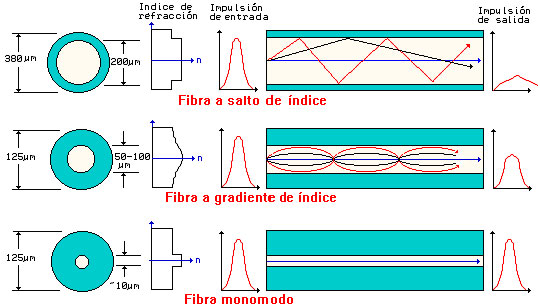
\includegraphics[width=0.66\linewidth]{Kap1/fibras3.jpg}
\caption{Tipos de fabricación tanto en escala-tamaño como en variación de índice de refracción en función del radio. Tomado de \textit{https://es.wikipedia.org/wiki/Fibra-optica}} 
\label{fibras3}
\end{figure} 
%sacada de: referencia

Por otro lado las fibras multimodo al tener un núcleo más grande permiten al haz de luz recorrer distintos caminos ópticos lo cual introduce dispersión modal, por esto existen dos tipos de fibras multimodo como se muestra en la figura \ref{fibras3}, las fibras de índice escalonado se compone de dos únicos materiales lo cual aumenta la dispersión modal y cromática (dichas fibras dadas sus limitaciones pero fácil construcción son usadas para enlaces cortos 100m). Ahora las fibras con gradiente de índice se construyen a partir de pequeños saltos de índice siguiendo una distribución parabólica de manera discreta puesto que por cuestiones de fabricación no es posible variar el índice de manera continua, dicha disposición contribuye a la reducción de la dispersión modal y dispersión cromática en función de la longitud de onda de la fuente aumentando el alcance al orden de 2km. Puesto que las fibras multimodo son para enlaces cortos tienden a tener un mayor rango de tolerancia en cuanto a fuentes con lo cual suelen venir optimizadas entre 800-1300 nm.\\

Puesto que los procesos de fabricación no son perfectos pueden presentarse perdidas de intensidad de la onda por dispersión o absorción propia del material, dentro de la dispersión se tienen varias contribuciones como ya se ha mencionado la dispersión cromática y modal, pero además se cuenta con un Scattering o dispersión de Rayleigh el cual se produce por la interacción de la luz con microscópicas irregularidades o estrés en el material producidas durante la fabricación del mismo, esto hace que la luz se disperse en otras direcciones incluso superando el ángulo critico siendo absorbida en el revestimiento.
Por ultimo tenemos la absorción la cual se da cuando la luz interactúa con átomos en el material usados para dopar y cambiar el índice de refracción al ser absorbido el fotón puede ser que el fotón emitido salga en otra dirección y se salga del núcleo terminando siendo absorbido en el revestimiento.

\begin{figure}[H]
\centering
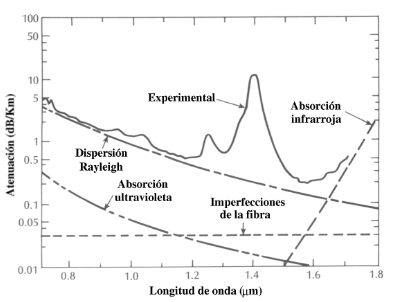
\includegraphics[width=0.56\linewidth]{Kap1/atenuacion.png}
\caption{Contribuciones en la atenuación de la onda en una fibra óptica en función de la longitud de onda de la fuente. Tomado de \textit{http://www.iuma.ulpgc.es/users/jrsendra/Docencia}.} 
\label{atenuacion}
\end{figure} 

En la figura \ref{atenuacion} se observan los efectos que producen atenuación de la señal en función de la longitud de onda según la región de operación de la fibra óptica. En el caso de la absorción suelen haber picos con la interacción de moléculas $OH+$ los cuales comúnmente se encuentran en los 1000, 1400 y 1600 nm creando ventanas en donde es óptima la transmisión, en éstas ventanas suelen trabajar las fibras monomodo y algunas multimodo de gradiente de índice.

%%%%----------------------------------------------%%%%
%%%%----------------------------------------------%%%%

\subsection{Teoría de difracción para las aberturas rectangular y circular.}

En esta sección se explicará la teoría básica de la abertura rectangular \textit{Slit} en inglés, y la abertura circular, los cuales son elementos ópticos importantes en el funcionamiento de cualquier espectrógrafo convencional. La teoría que presentamos acá está basada en la aproximación de Fraunhofer, es decir, el ancho de la abertura es mucho menor a la distancia entre el plano que contiene la abertura y el plano donde mediremos el patrón de difracción producido, esto es

\begin{equation}\label{aprox_fran}
    N=\left[ \frac{{(x+y)}^2}{2d}\right]\frac{2}{\lambda}\ll 1,
\end{equation}
donde $N$ es el número de zonas de Fresnel, &(x,y)& describen la abertura y $d$ la distancia entre los planos.\\

Para calcular el patrón de difracción producido por los orificios usaremos la integral de difracción de Fraunhofer, la cual es una aproximación generada de la integral de difracción de Fresnel aplicando la ecuacion (\ref{aprox_fran}), esto puede ser visto como el número de zonas de Fresnel que caben en la apertura con $N\ll 1$, dicha expresión está escrita de la siguiente manera:

\begin{equation}\label{difraccion_fraunhofer}
    I(x',y')=I(u\lambda d,v\lambda d)=\frac{1}{\lambda^2 d^2}|\mathcal{F}\lbrace E(x,y) \rbrace |^2 ,
\end{equation}
en la cual las variables primadas $(x',y')$ se ubican en un plano paralelo separado una distancia $d$ al plano donde se encuentra la abertura con variables $(x,y)$, dicho esto veamos como se procede a calcular la irradiancia para las aberturas de interés.

\begin{itemize}
    \item \textbf{Rendija rectangular.}\\
    Dada la simetría para la abertura rectangular, haremos de coordenadas cartesianas para expresar el campo eléctrico en el plano de la abertura, haciendo uso de la función rectángulo $rect(x)$ tenemos,
    \begin{equation}\label{campo_rect}
        E(x,y)=E_0 \hspace{2mm} rect(x/a) \hspace{2mm} rect(y/b)\hspace{5mm}\text{ donde }\hspace{5mm}rect(x/a) = \left\lbrace
        \begin{array}{ll}
            \textup{si } |x|\leq a/2 & 1\\
            \textup{si } |x| > a/2 & 0
        \end{array}
        \right.
    \end{equation}
    
        \begin{figure}[H]
    \centering
    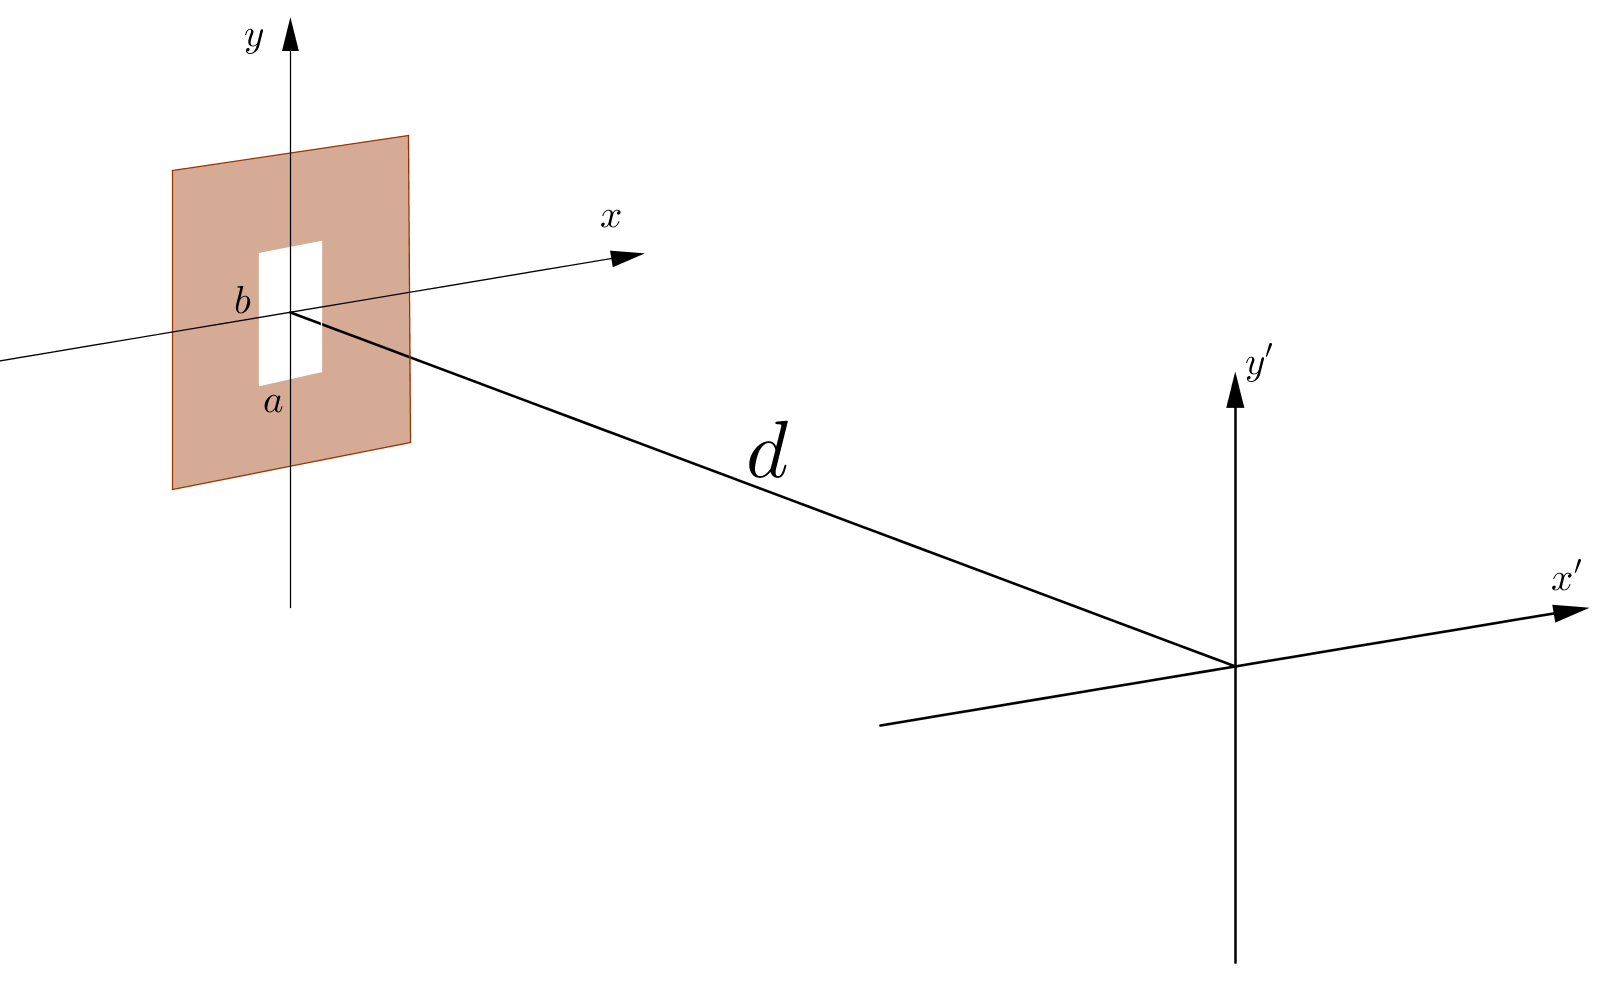
\includegraphics[width=0.75\linewidth]{Kap1/apertura_rect.png}
    \caption{Esquema  apertura rectangular aproximación de Fraunhofer.} 
    \label{abertura_rect}
    \end{figure}
    
    En la figura \ref{abertura_rect} se muestra la situación planteada, con lo cual una vez expresado el campo $E$ procedemos a hallar la irradiancia $I$ usando la ecuación (\ref{campo_rect}) en (\ref{difraccion_fraunhofer}) de la siguiente manera
    
    \begin{eqnarray}
        I(x',y')&=&\frac{1}{\lambda^2 d^2} \left |\int_{-\infty}^{\infty} \int_{-\infty}^{\infty} E(x,y) e^{-2\pi i (ux+vy)}dx dy \right |^2\\
        &=&\frac{1}{\lambda^2 d^2} \left |\int_{-a/2}^{a/2} \int_{-b/2}^{b/2} E_0 e^{-2\pi i (ux+vy)}dx dy \right |^2\\
        &=&\frac{E_0}{\lambda^2 d^2} \left |\int_{-a/2}^{a/2} e^{-2\pi i ux} dx\int_{-b/2}^{b/2} e^{-2\pi i vy} dy \right |^2,
    \end{eqnarray}
    
    calculando la integral en $x$ (de manera similar para $y$) 
    
    \begin{eqnarray}
        \int_{-a/2}^{a/2} e^{-2\pi i ux} dx &=&\left\frac{-1}{2\pi i u}  e^{-2\pi i ux}\right |_{-a/2}^{a/2} = \frac{-i}{2\pi u}\left[ -e^{-\pi i ua} + e^{\pi i ua}\right] \\ 
         &=&\frac{-i(2i)}{2\pi u}\sin{(\pi u a)}\frac{a}{a} = a \hspace{1mm} sinc(\pi x'a/\lambda d),
    \end{eqnarray}

    con lo cual finalmente se obtiene la expresión 
    
    \begin{equation}
        I(x',y')=I_0 \hspace{1mm}{sinc}^2\left(\frac{\pi x' a}{\lambda d} \right) \hspace{1mm}{sinc}^2\left(\frac{\pi y' b}{\lambda d} \right)\hspace{4mm}\text{ con }\hspace{4mm} I_0=\frac{E_0^2 a^2 b^2}{\lambda^2 d^2}
    \end{equation}
    
    \begin{figure}[H]
    \centering
    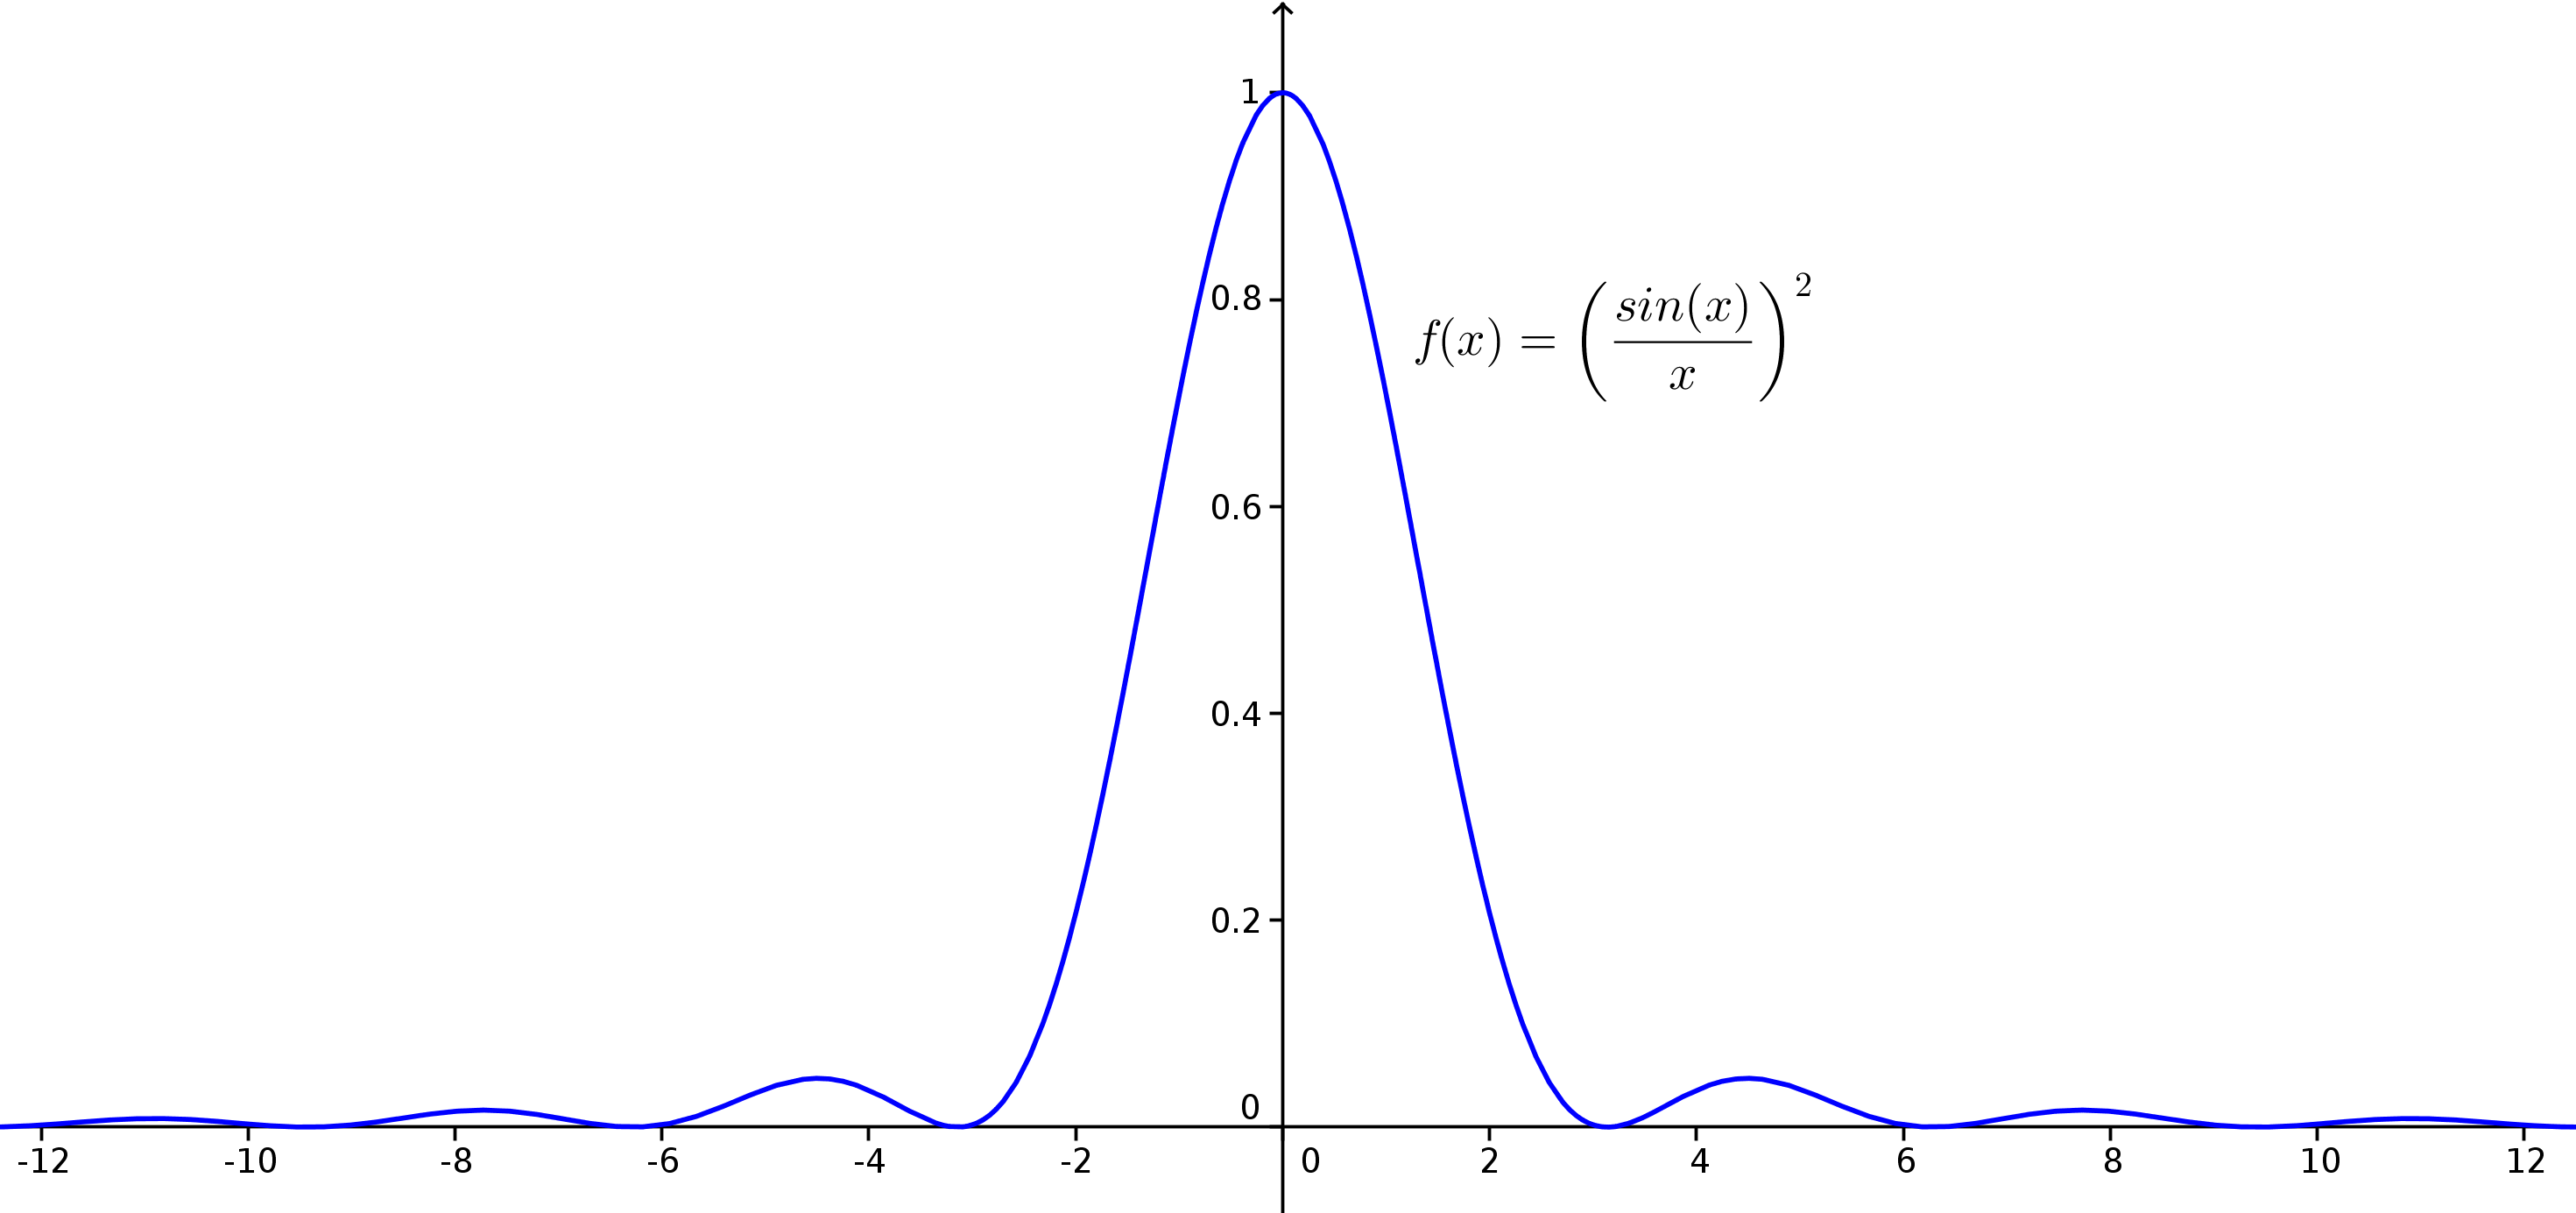
\includegraphics[width=0.75\linewidth]{Kap1/sinc.png}
    \caption{Gráfica de la función ${sinc}^2(x)$.} 
    \label{sinc}
    \end{figure}
    
    la ecuación (\ref{irrad_rect}) nos muestra el patrón de difracción generado por la abertura, donde se observan máximos y mínimos de radiación modulados por una función seno en cada eje. Como ejemplo se tiene al \textbf{Slit} el cual puede tener el orden de pocos centímetros de alto y un orden de micras de ancho, es decir, se observa con mayor claridad un patrón en una dirección que en otra. la figura \ref{sinc} describe el comportamiento de la función ${sinc}^2(x)$ la cual tiene un máximo de irradiancia en el origen y se puede ver como un patrón unidimensional similar al Slit.
    
    \item \textbf{Apertura circular.}\\
    
    \begin{figure}[H]
    \centering
    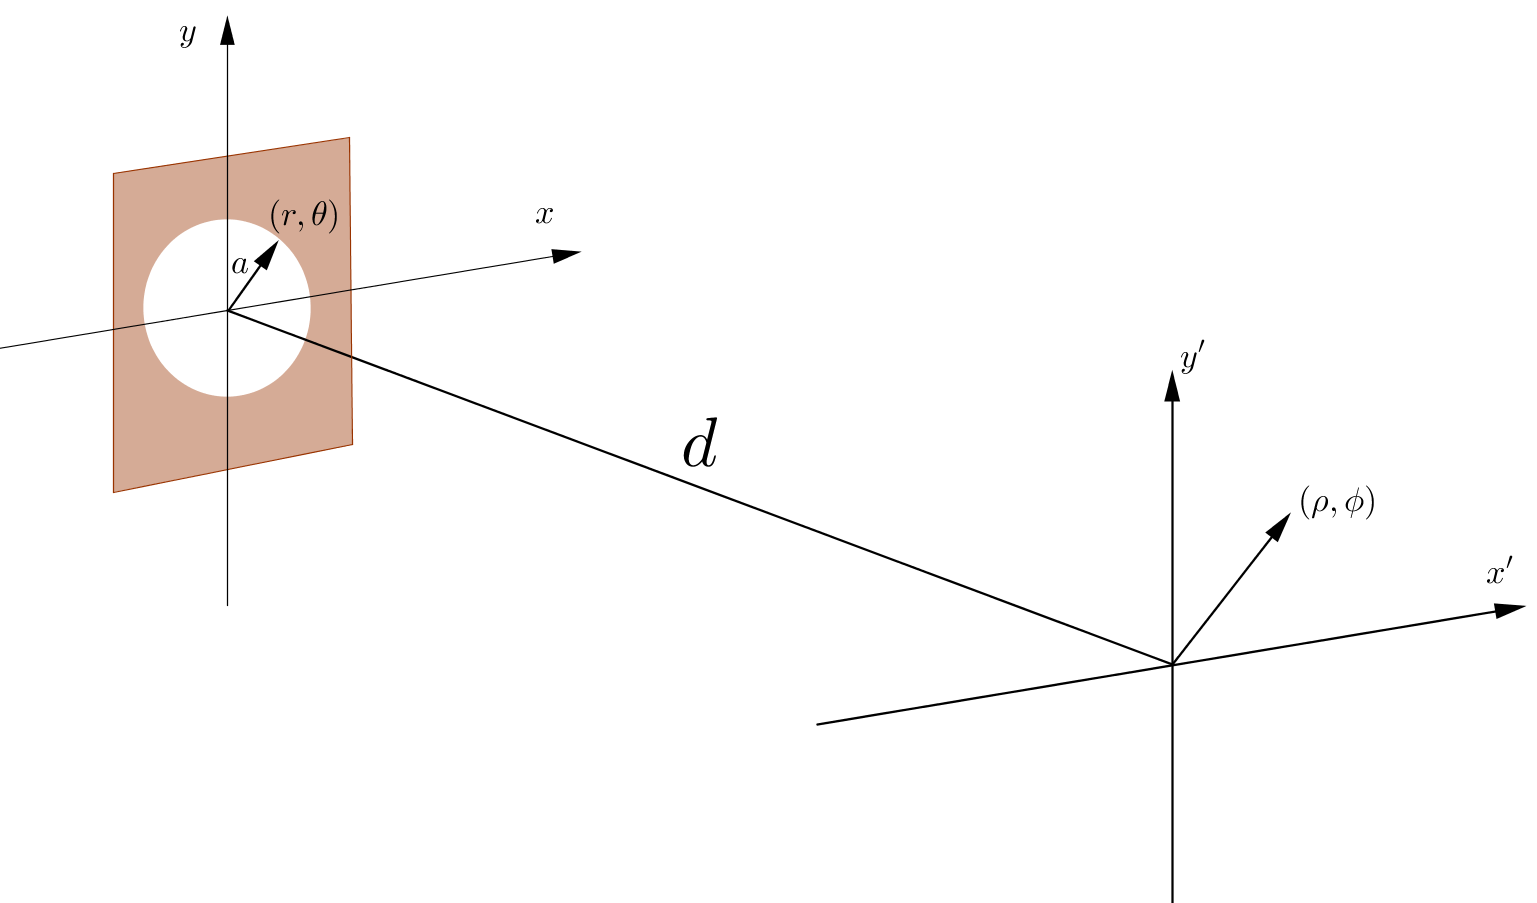
\includegraphics[width=0.75\linewidth]{Kap1/apertura_circ.png}
    \caption{Esquema  apertura circular aproximación de Fraunhofer.} 
    \label{esq_circular}
    \end{figure}
    
    En la figura \ref{esq_circular} se observa la simetría del problema en cuestión,como se ha visto la geometría de la abertura influye en el desarrollo de los cálculos por lo cual será más conveniente usar un sistema de coordenadas polar. Realizando un cambio de variables de la forma
    
    \begin{eqnarray}
        x&=&r\cos{\theta} \hspace{5mm} u=\rho \cos{\phi} \hspace{5mm} \rho = \sqrt{\frac{{x'}^2+{y'}^2}{\lambda ^2 d^2}}\\
        y&=&r\sin{\theta} \hspace{5mm} v=\rho \sin{\phi}.
    \end{eqnarray}
    Así pues,
    \begin{eqnarray}
        E(x',y')&=&\iint_{-\infty}^{\infty} E_0 circ\left( \frac{(x^2+y^2)^{1/2}}{a} \right) e^{-2\pi i(ux+vy)} dx dy\\
        E(\rho,\phi)&=& \int_{0}^{a} \int_{0}^{2\pi} E_0 e^{-2\pi i(\rho r \cos{\phi}\cos{\theta}+\rho r \sin{\phi}\sin{\theta})}rdrd\theta \\
        E(\rho,\phi)&=&E_0\int_{0}^{a} \int_{0}^{2\pi}e^{-2\pi i\rho r \cos{(\phi - \theta)}}rdrd\theta.
    \end{eqnarray}
    
    Usando la expresión de la función de Bessel de orden cero
    
    \begin{equation}
        J_0(u)=\frac{1}{2\pi}\int_{0}^{2\pi}e^{i u \cos{v}}dv,
    \end{equation}
    
    entonces la expresión para el campo queda
    
    \begin{equation}\label{campo_polares}
        E(\rho,\phi) = E_0 \frac{2\pi}{\lambda d} \int_{0}^{a} J_0(2\pi \rho r)rdr.
    \end{equation}
    Ahora usando la relación de recurrencia para las funciones de Bessel
    
    \begin{equation}\label{recurrencia_bessel}
        \frac{d}{du}\left[u^m J_m(u)\right]=u^m J_{m-1}(u) \hspace{4mm}\text{ para m=1  }\hspace{3mm} \frac{d}{du}\left[u J_1(u)\right]=u J_{0}(u),
    \end{equation}
    con lo cual usando (\ref{recurrencia_bessel}) en la ecuación (\ref{campo_polares}) solo queda evaluar la integral entre $0$ y $a$ quedando
    
    \begin{eqnarray}
        E(\rho,\phi)&=& E_0\frac{2\pi}{\lambda d} a^2 J_1(2\pi \rho a)\frac{1}{2\pi \rho a}\\
        E(\rho)&=& \left[ \frac{\pi a^2 E_0}{\lambda d}\right]\frac{2J_1(2\pi \rho a)}{2\pi \rho a},
    \end{eqnarray}
    con lo cual finalmente hallando el modulo al cuadrado para hallar la irradiancia tenemos
    
    \begin{equation}\label{irrad_circ}
        I(\rho)=I_0\left[\frac{2J_1(2\pi \rho a)}{2\pi \rho a}\right]^2  \hspace{3mm} \xrightarrow{\;\; \rho=r/\lambda d \;\; } \hspace{3mm}  I(r)=I_0\left[\frac{2J_1(\pi ar/\lambda d)}{(\pi ar/\lambda d)}\right]^2,
    \end{equation}
    la ecuación (\ref{irrad_circ}) nos muestra la irradiancia donde se observa una simetría en $\phi$ , es decir, el patrón generado serán anillos concéntricos. De ésta misma ecuación al igualar el primer cero de $J_1$ con su argumento, nos encontramos con la relación $r_a=1.22 \lambda d /a$, donde $r_a$ es llamado el \textbf{radio de Airy} y es precisamente la primera región de difracción para la abertura circular.\\
    De lo anterior nace el criterio de Rayleigt en el cual se indica que dos fuentes puntuales son resueltas por un observador si los centros de sus anillos de Airy están separados una distancia mayor a $r_a$.
\end{itemize}


\subsection{Rejilla de difracción.}
Las rejillas de difracción son un elemento óptico clave en cualquier instrumento de espectrometría, ya que con ella podemos descomponer la luz incidente en todas sus longitudes de onda constituyentes. Existen diversos tipos de rejillas con diferentes geometrías y materiales con lo cuales se obtiene una optimización en un rango del espectro electromagnético de interés. A continuación observaremos cuál es el principio teórico de manera muy similar a las aberturas circular y rectangular.\\

\begin{figure}[H]
    \centering
    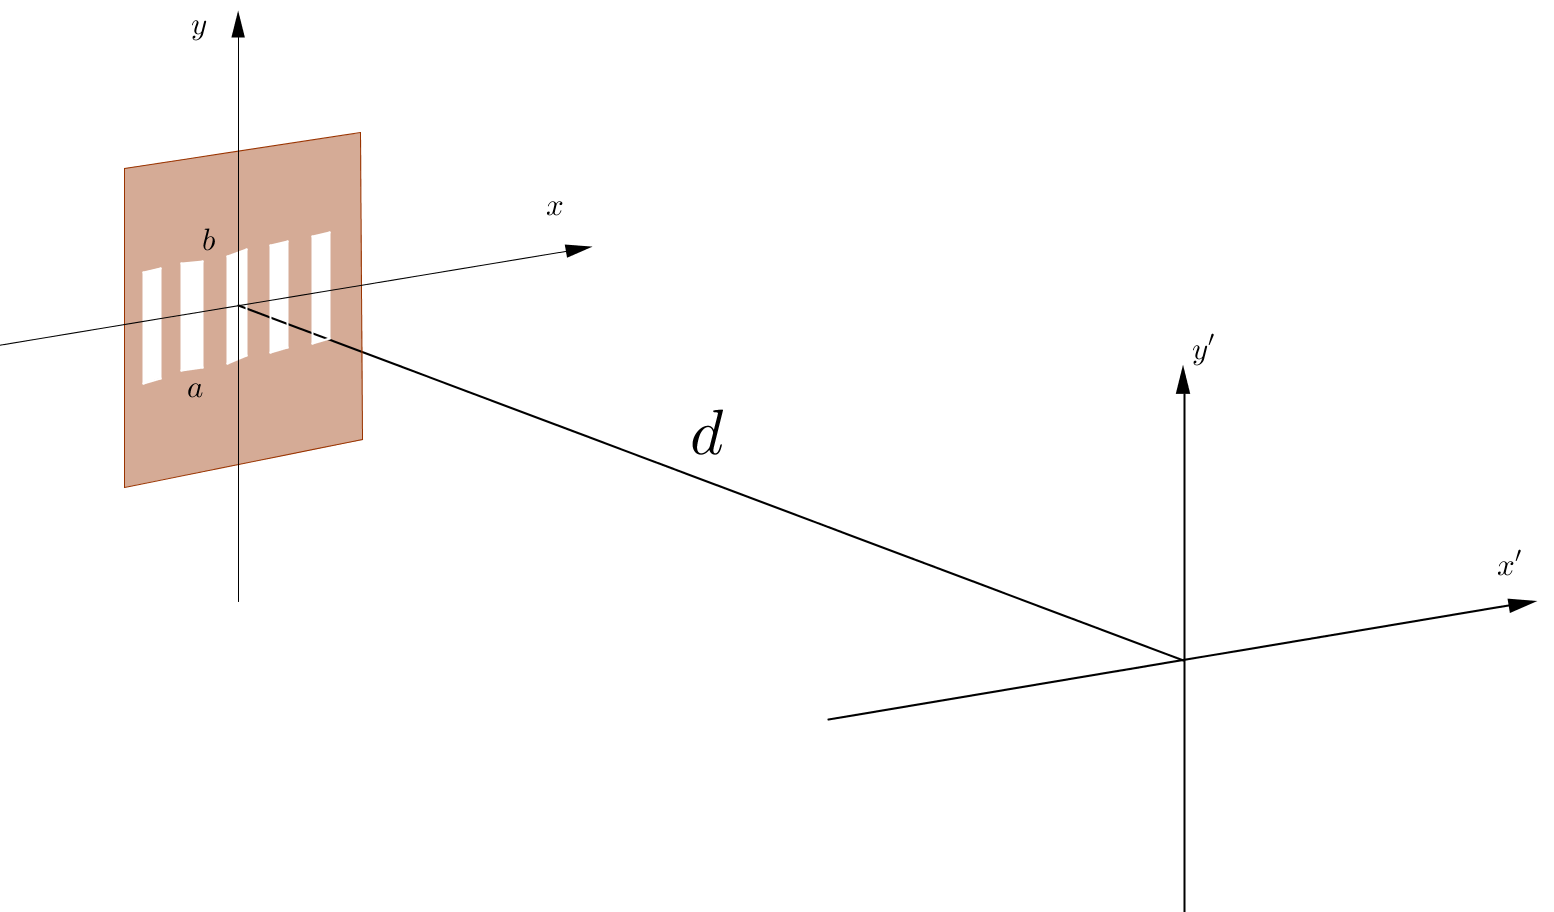
\includegraphics[width=0.8\linewidth]{Kap1/apertura_rejilla.png}
    \caption{Esquema para la rendija múltiple.} 
    \label{esq_rejilla}
\end{figure}
Como se observa en la figura \ref{esq_rejilla}, la rejilla se compone de $N$ rendijas rectangulares de ancho $a$ separadas una distancia $b$; con esta idea y usando la aproximación de Fraunhofer podemos superponer la solución ya encontrada para la apertura rectangular, con lo cual definimos la función rectángulo de la siguiente manera

\begin{equation}
    rect\left(\frac{x}{x_0}\right)=\left\lbrace
    \begin{array}{ll}
        \textup{si } |x|\leq {x_0}/2 & 1\\
        \textup{si } |x| \textup{ en otro caso.}
    \end{array}
    \right.
\end{equation}
Puesto que las aberturas se encuentran organizadas a lo largo del eje $x$, calcularemos la irradiancia que se produce a lo largo de este eje; de esta forma el campo $E$ en la dirección $x$ será el producto de la función rectángulo para una abertura desplazada $N$ veces, es decir, la convolución 

\begin{equation}\label{campo_rejilla}
    E(x)=E_0 \hspace{1mm} rect\left(\frac{x}{a}\right) \ast \sum_{n=0}^{N-1}\delta(x-nb) ,
\end{equation}
donde $N$ es el número de aberturas, $a$ el ancho y $b$ la separación entre los centros de las mismas.\\
Ahora aplicando la transformada de Fourier al campo y usando las propiedades de la convolución tenemos

\begin{eqnarray}\label{transf_rejilla}
    \mathcal{F}\lbrace E(x)\rbrace&=&\mathcal{F}\left \{ rect\left(\frac{x}{a}\right)\right \}\mathcal{F}\left \{ \sum_{n=0}^{N-1}\delta(x-nb)\right \}\\
    &=& a\hspace{1mm}sinc(\pi x' a) \left[ \sum_{n=0}^{N-1} e^{-2\pi i nbx'} \right].
\end{eqnarray}

Ahora calculando la suma mediante la resta de series tenemos

\begin{equation}
    S=\sum_{n=0}^{N-1} e^{-2\pi i nbx'} \hspace{10mm}S e^{-2\pi i bx'} = \sum_{n=1}^{N} e^{-2\pi i nbx'},
\end{equation}

con lo cual restando las series se obtiene

\begin{eqnarray}
    S\left(1-e^{-2\pi i bx'}\right)&=&1-e^{-2\pi i Nbx'}\\
    S&=&\frac{1-e^{-2\pi i Nbx'}}{1-e^{-2\pi i bx'}}=\frac{e^{-\pi i Nbx'}\left(e^{\pi i Nbx'}-e^{-\pi i Nbx'}\right)}{e^{-\pi i bx'}\left(e^{\pi i bx'}-e^{-\pi i bx'}\right)}\\
    S&=&e^{-\pi i (N-1) bx'}\left[\frac{\sin{(\pi N bx')}}{\sin{(\pi  bx')}}\right],
\end{eqnarray}

asi retomando la ecuación (\ref{transf_rejilla}) y hallando el módulo al cuadrado obtenemos 

\begin{equation}\label{irrad_rejilla}
    I(x')=I_0\hspace{1mm}{sinc}^2(\pi x' a) e^{-2\pi (N-1) bx'}\left[ \frac{\sin{(\pi N bx')}}{\sin{(\pi  bx')}} \right]^2 \hspace{3mm}\text{con}\hspace{3mm}I_0=\frac{E_{0}^{2} a^2}{\lambda^2 d^2},
\end{equation}
si suponemos muchas aberturas, $N\rightarrow\infty$
\begin{equation}\label{irrad_rejilla_Ngrande}
    I(x')=I_0\hspace{1mm}{sinc}^2(\pi x' a) \left[ \frac{\sin{(\pi N bx')}}{\sin{(\pi  bx')}} \right]^2,
\end{equation}
finalmete la ecuación (\ref{irrad_rejilla_Ngrande}) nos describe el patrón de difracción para la rejilla constituida por múltiples aberturas, esta ecuación nos muestra por un lado el valor máximo $I_0$ que puede tomar la función, otro término que expresa la irradiancia generada a partir de una única abertura y un término final correspondiente a la interferencia generada por las $N$ aberturas.
%%%%%----------------------------------------------%%%%%
%%%%----------------------------------------------%%%%

\subsection{Integrated Fiber Unit (IFU).}

En la actualidad existen dispositivos tanto de imagen como espectrógrafos que utilizan múltiples fibras ópticas en el diseño de los mismos. A los instrumentos que usan este enjambre de fibras ópticas se les conoce como IFU, acrónimo en inglés correspondiente a \textit{Integrated Fiber Units}. Un ejemplo de estos es el instrumentos SINFONI \textit{Spectrometer for Infrared Faint Field Imaging}.\\
Además de SINFONI se encuentran en desarrollo e incluso construcción diversos instrumentos los cuales desean obtener información espectroscópica de algún objeto astronómico en un mismo instante de tiempo, en éste caso el objeto de interés es el Sol el cual nos lleva a superar diversos retos puesto que es una fuente de gran intensidad. Superando éstos desafíos a la hora de obtener información del Sol se expondrán 3 proyectos IFU's con cualidades ópticas diferentes \textbf{multi Slit}, \textbf{multi fibra} y \textbf{multi lentes}, los cuales proponen construir imágenes del Sol con gran resolución espacial y espectral en un amplio rango de longitudes de onda (hacia el IR cercano), éstos instrumentos están diseñados para telescopios terrestres.\\

El primer instrumento \textbf{multi Slit} llamado \textbf{MuSICa} \textit{Multi Slit Image Slicer on collimator Camera} del IAC, diseñado para el telescopio terrestre Gregor de 1,5m se compone de una mascara dividida en 2 segmentos, con lo cual cada segmento de la imagen es dirigido con ayuda de espejos a una mascara con 4 slits, nuevamente cada slit es redirigido con ayuda de espejos a una disposición vertical donde finalmente la luz es dispersada por una rejilla de reflexión cóncava esférica y registrada con un detector igualmente cóncavo esférico. Así se obtiene una imagen compuesta por 8 slits con un ancho de 100 $\mu$m y altura 1,8 mm, el hecho de que la luz no atraviesa ningún elemento óptico disminuye los efectos de aberración generando una mayor calidad de la imagen espectroscópica.\\ 

El segundo instrumento \textbf{multi fibra} es diseñado para el telescopio de 4m DKIST, en este caso se cuentan con diversos proyectos con longitudes de onda en el rango visble e IR cercano y lejano. Pero en especial hablaremos del \textbf{DL-NIRSP} "Diffraction-Limited-Near-Infrared SP" del NSO.

\begin{figure}[H]
\centering
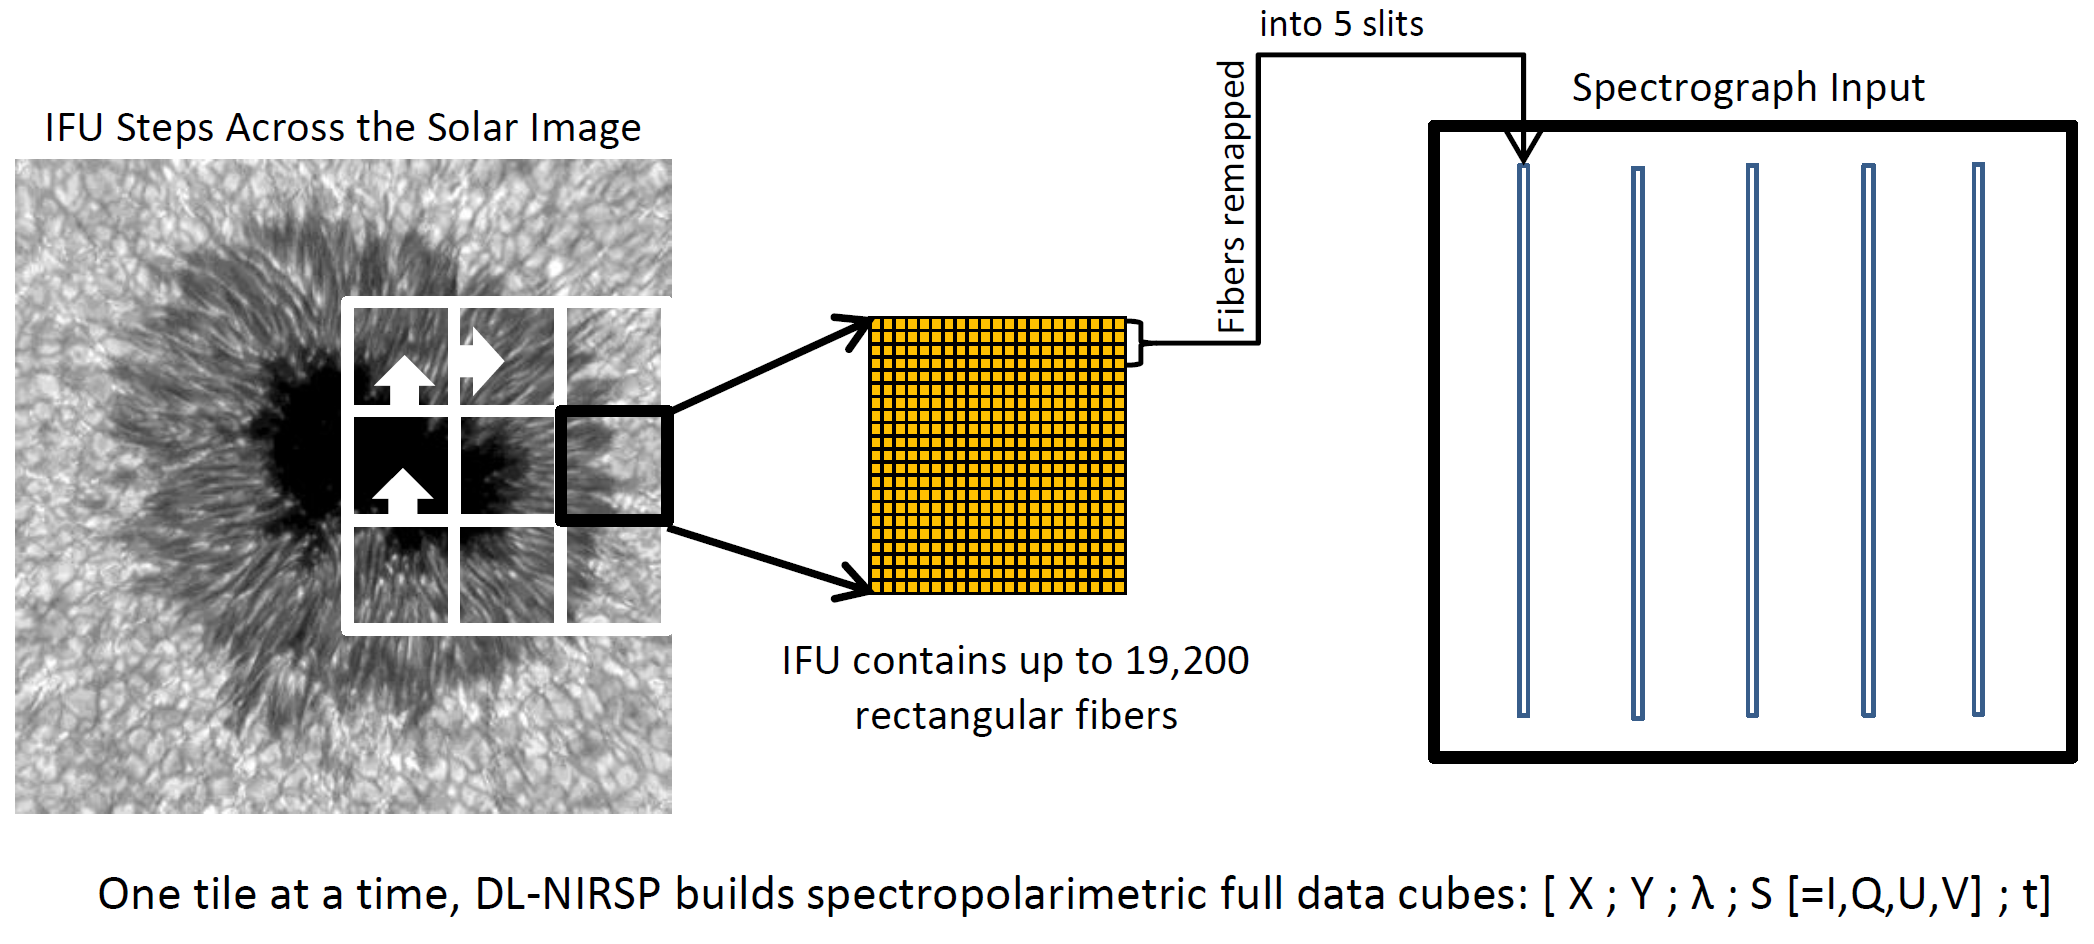
\includegraphics[width=0.70\linewidth]{Kap1/nirsp.png}
\caption{Esquema del funcionamiento para el instrumento DL-NIRSP del NSO. Tomado de \textit{https://www.nso.edu/telescopes/dkist/instruments/dl-nirsp}} 
\label{nirsp}
\end{figure}

Como se observa en la figura \ref{nirsp} el instrumento cuenta con un arreglo de fibras cuadradas (19200) con las cuales se mapea la región del Sol en interés (9 zonas), después las fibras son organizadas en un arreglo lineal de 5 Slit donde posteriormente se descompone la luz con ayuda de una rejilla de reflexión cóncava que finalmente será registrada por el detector. Dicha disposición logra que el instrumento tenga un campo de visión de 120x120 arcsec y una resolución espectral $R\aprox250000$ analizando estados Full de polarización de las lineas espectrales en la rango 900-2500 nm con una cadencia temporal menor a 100 ms, dado éste rango de operación el instrumento estudia la cromosfera Solar en regiones activas donde pueden producirse Flares.\\

Por último el instrumento \textbf{multi lentes} denominado \textbf{Mihi} del MPS el cual se compone de un arreglo de fibras ópticas que a su vez cuentan con microlentes los cuales reducen el tamaño del píxel al capturar mayor información en el plano imagen del telescopio.

\begin{figure}[H]
\centering
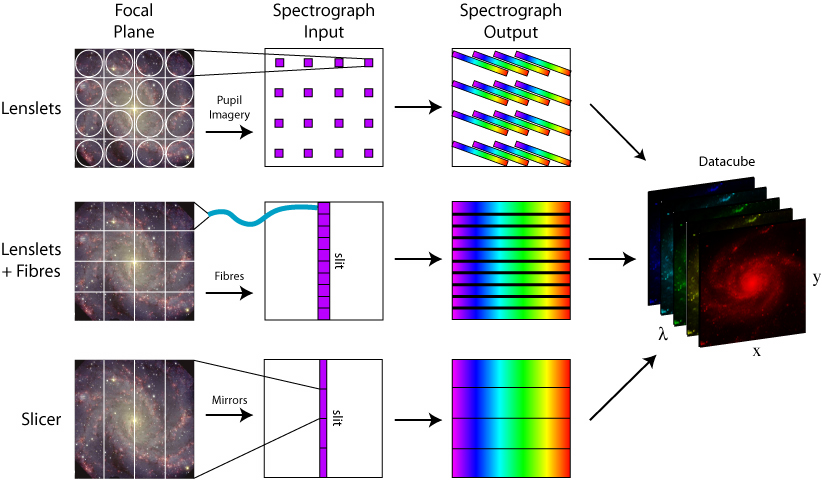
\includegraphics[width=0.70\linewidth]{Kap1/multilentes.jpg}
\caption{Diferencias en el diseño para la obtención de datos en los diferentes IFU's. M. Westmoquette, adapted from Allington-Smith et al. 1998 ,Recuperado de \textit{http://ifs.wikidot.com}.} 
\label{multilente}
\end{figure}

El funcionamiento en éste caso es muy similar al DL-NIRSP como se muestra en la figura \ref{multilente}, con la diferencia que se añaden microlentes para capturar más información, el transporte de la información también se da por fibra óptica al igual que el uso de una rejilla de reflexión y detector cóncavos. Al introducir microlentes se añade una dispersión espectral como se ejemplifica en la figura \ref{multilente} lo cual hace que se tengan que usar nuevos algoritmos para la obtención final de datos.





\chapter{Marco teórico.}

\section{efectos físicos relevantes.}


\section{Método de MonteCarlo.}

Es una técnica numérica utilizada para calcular probabilidades y otras cantidades relacionadas, utilizando secuencias de números aleatorios (AGREGAR CITACIÓN). La efectividad de este metodo depende en gran medida de un buen generador de numeros aleatorios, por ende, dicho método tomó importancia a partir de la producción en masa de las computadoras. Pues estás son buenas generadoras de numeros aleatorios. 

\section{Geant4.}
Geant4 es un conjunto de herramientas que se utilizan en el estudio de interacción materia. Tiene una gran variedad de áreas de aplicación, las cuales incluyen la física de altas energías, nuclear y de aceleradores, así como estudios en ciencias médicas y espaciales. No es objetivo de este documento explicar de manera detalla el uso y funcionamiento de Geant4, sin embargo, se hará una breve explicación de los aspectos mas relevantes.



\chapter{Aspectos generales de los Morteros.}

\section{Características.}

Como un primer acercamiento al estudio de materiales de construcción se elaboraron 5 lotes de morteros, cuyas composiciones son distintas. Inicialmente cada lote consta de 4 placas. Es importante mencionar que estos no cumplen ningún tipo de reglamentación oficial. En las simulaciones realizadas para transmisión se colocan 10 placas y para retrodispersión 13. El lote de morteros 5 se empezará a analizar en detalle en el capitulo 6, pues en este se hacen las comparaciones entre simulación y experimento. 

(AGREGAR FORMA DE LOS MORTEROS.)

En las siguientes tablas se muestran las dimensiones de las placas correspondientes a cada lote. Estos tienen la forma que se muestra en la figura \ref{Fig:Diagrama-Mortero}.


\begin{table}[H]
	\centering
	\begin{tabular}{|c|c|c|c|c|c|c|c|}
		\hline
		\multicolumn{8}{|c|}{Laminas de Morteros1}                                                                             \\ \hline
		\multirow{Lamina \#} & Masa {[}g{]} & H1 {[}cm{]} & H2 {[}cm{]} & L1 {[}cm{]} & L2 {[}cm{]} & W1 {[}cm{]} & W2 {[}cm{]} \\ \cline{2-8} 
		& (+/- 0.01)   & \multicolumn{6}{c|}{(+/- 0.001)}                                                  \\ \hline
		1                          & 136.28       & 9.666      & 9.745      &9.663        & 9.647      & 0.886       & 0.916       \\ \hline
		2                          & 142.01       & 9.684      & 9.714      & 9.636       & 9.681      & 0.858       & 0.959       \\ \hline
		3                          & 145.92       & 9.726      & 9.572      & 9.579       & 9.546      & 0.880       & 1.069       \\ \hline
		4                          & 138.57       & 9.736      & 9.704      & 9.581       & 9.585      & 0.934       & 1.016       \\ \hline
	\end{tabular}
	\caption{Medidas experimentales del lote morteros1.}
	\label{t:medidas-morteros1}
\end{table}


 \begin{table}[H]
 	\centering
 	\begin{tabular}{|c|c|c|c|c|c|c|c|}
 		\hline
 		\multicolumn{8}{|c|}{Laminas de Morteros2}                                                                             \\ \hline
 		\multirow{Lamina \#} & Masa {[}g{]} & H1 {[}cm{]} & H2 {[}cm{]} & L1 {[}cm{]} & L2 {[}cm{]} & W1 {[}cm{]} & W2 {[}cm{]} \\ \cline{2-8} 
 		& (+/- 0.01)   & \multicolumn{6}{c|}{(+/- 0.001)}                                                  \\ \hline
 		1                          & 149.35       & 9.760       & 9.706      &9.518         & 9.523      & 0.757       & 0.974       \\ \hline
 		2                          & 157.36       & 9.742       & 9.753      &9.564         & 9.624      & 0.955       & 0.991       \\ \hline
 		3                          & 151.53       & 9.742       & 9.722      &9.615         & 9.493      & 0.923       & 0.956       \\ \hline
 		4                          & 136.97       & 9.757       & 9.794      &9.577         & 9.528      & 0.871       & 0.921       \\ \hline
 	\end{tabular}
 	\caption{Medidas experimentales del lote morteros2.}
 	\label{t:medidas-morteros2}
 \end{table}

  \begin{table}[H]
 	\centering
 	\begin{tabular}{|c|c|c|c|c|c|c|c|}
 		\hline
 		\multicolumn{8}{|c|}{Laminas de Morteros3}                                                                             \\ \hline
 		\multirow{Lamina \#} & Masa {[}g{]} & H1 {[}cm{]} & H2 {[}cm{]} & L1 {[}cm{]} & L2 {[}cm{]} & W1 {[}cm{]} & W2 {[}cm{]} \\ \cline{2-8} 
 		& (+/- 0.01)   & \multicolumn{6}{c|}{(+/- 0.001)}                                                  \\ \hline
 		1                          & 148.71       & 9.825        & 9.820      & 9.583         & 9.712      & 0.975       & 0.935       \\ \hline
 		2                          & 150.32       & 9.672        & 9.616      & 9.528         & 9.577      & 0.968       & 0.929       \\ \hline
 		3                          & 139.83       & 9.613        & 9.640      & 9.463         & 9.521      & 0.949       & 0.916       \\ \hline
 		4                          & 133.72       & 9.864        & 9.839      & 9.526         & 9.550      & 0.852       & 0.916       \\ \hline
 	\end{tabular}
 	\caption{Medidas experimentales del lote morteros3.}
 	\label{t:medidas-morteros3}
 \end{table}
 
 
    \begin{table}[H]
 	\centering
 	\begin{tabular}{|c|c|c|c|c|c|c|c|}
 		\hline
 		\multicolumn{8}{|c|}{Laminas de Morteros4}                                                                             \\ \hline
 		\multirow{Lamina \#} & Masa {[}g{]} & H1 {[}cm{]} & H2 {[}cm{]} & L1 {[}cm{]} & L2 {[}cm{]} & W1 {[}cm{]} & W2 {[}cm{]} \\ \cline{2-8} 
 		& (+/- 0.01)   & \multicolumn{6}{c|}{(+/- 0.001)}                                                  \\ \hline
 		1                          & 156.90       & 9.774         & 9.804      & 9.557          & 9.563      & 0.938       & 10.20       \\ \hline
 		2                          & 145.96       & 9.687         & 9.653      & 9.620          & 9.550      & 0.914       & 0.940       \\ \hline
 		3                          & 140.52       & 9.657         & 9.693      & 9.579          & 9.589      & 1.079       & 0.902       \\ \hline
 		4                          & 147.33       & 9.814         & 9.772      & 9.546          & 9.589      & 1.075       & 0.953       \\ \hline
 	\end{tabular}
 	\caption{Medidas experimentales del lote morteros4.}
 	\label{t:medidas-morteros4}
 \end{table}
 
 
     \begin{table}[H]
 	\centering
 	\begin{tabular}{|c|c|c|c|c|c|c|c|}
 		\hline
 		\multicolumn{8}{|c|}{Laminas de Morteros5}                                                                             \\ \hline
 		\multirow{Lamina \#} & Masa {[}g{]} & H1 {[}cm{]} & H2 {[}cm{]} & L1 {[}cm{]} & L2 {[}cm{]} & W1 {[}cm{]} & W2 {[}cm{]} \\ \cline{2-8} 
 		& (+/- 0.01)   & \multicolumn{6}{c|}{(+/- 0.001)}                                                  \\ \hline 		1                          & 136.58       & 9.762          & 9.734      & 96.67         & 96.10       & 1.009       & 0.877       \\ \hline
 		2                          & 133.28       & 9.660          & 9.646      & 96.00         & 96.42       & 0.850       & 0.887       \\ \hline
 		3                          & 128.12       & 9.629          & 9.673      & 95.11         & 95.30       & 0.927       & 0.824       \\ \hline
 		4                          & 130.35       & 9.670          & 9.677      & 95.77         & 96.93       & 0.869       & 0.912       \\ \hline
 	\end{tabular}
 	\caption{Medidas experimentales del lote morteros5.}
 	\label{t:medidas-morteros5}
 \end{table}
 
 Otro dato importante es la densidad del material, por ello se calcula de densidad de los morteros mediante la ecuación (\ref{densidad-mor1}).  Es importante mencionar que esta densidad es calculada para todas las placas por mortero, es decir, se tomó un lote y se le calculó el promedio de la masa y de las diferentes dimensiones, y con estos nuevos valores se hizo el cálculo. Este mismo proceso se repite para todos.

\begin{equation} \label{densidad-mor1}
    \begin{split}
	    \rho=\frac{masa}{volumen}
	\end{split}
\end{equation}

\begin{table}[H]
    \begin{center}
        \begin{tabular}{| c | c | }
            \hline
            Lote de Morteros & densidad (g/cm^3) \\ \hline
            1 & 1.62(4)  \\
            2 & 1.75(5) \\
            3 & 1.62(7) \\
            4 & 1.62(3) \\
            5 & 1.60(6) \\ \hline
        \end{tabular}
    \caption{Densidad de los diferentes Morteros.}
    \label{t:densi-morteros}
\end{center}
\end{table} 


También es necesario saber cuales son las composiciones y el porcentaje empleado en cada lote, así que en las tablas \ref{t:materiales-morteros1}, \ref{t:materiales-morteros2}, \ref{t:materiales-morteros3}, \ref{t:materiales-morteros4}, \ref{t:materiales-morteros5} muestras dichas composiciones. La composición para cada lote fue elegida de acuerdo a la utilidad que tiene en la práctica, es decir, se escogieron las mezclas mas usadas en las construcciones. Pues de acuerdo a lo que se desee construir se tiene una u otra mezcla. Todas las características proporcionadas son necesarias para construir las placas de morteros en Geant4.


\begin{multicols}{2}

\begin{table}[H]
	\centering
	\begin{tabular}{|c|c|c|}
		\hline
		\multirow{Material Mortero1} & \multicolumn{2}{c|}{4 placas} \\ \cline{2-3}
		& g         	& \%        	\\ \hline
		Cemento Portland      	& 320      	& 39.024    	\\ \hline
		Arena Peña         	& 300      	& 36.585    	\\ \hline
		Agua                  	& 200     	& 24.340     	\\ \hline
	\end{tabular}
	\caption{Proporción porcentual en la \\ 
	elaboración de morteros1.}
	\label{t:materiales-morteros1}
\end{table}


 \begin{table}[H]
 	\centering
 	\begin{tabular}{|c|c|c|}
 		\hline
 		\multirow{Material Mortero2} & \multicolumn{2}{c|}{4 placas} \\ \cline{2-3}
 		& g         	& \%        	\\ \hline
 		Cemento Portland      	& 160      	& 22.535    	\\ \hline
 		Arena Peña         	& 450      	& 63.380    	\\ \hline
 		Agua                  	& 100     	& 14.084     	\\ \hline
 	\end{tabular}
 	\caption{Proporción porcentual en la \\
 	elaboración de morteros2.}
 	\label{t:materiales-morteros2}
 \end{table}



  \begin{table}[H]
 	\centering
 	\begin{tabular}{|c|c|c|}
 		\hline
 		\multirow{Material Mortero3} & \multicolumn{2}{c|}{4 placas} \\ \cline{2-3}
 		& g         	& \%        	\\ \hline
 		Cemento Portland      	& 110      	& 15.492    	\\ \hline
 		Arena Sílice         	& 500      	& 70.422    	\\ \hline
 		Agua                  	& 100     	& 14.084     	\\ \hline
 	\end{tabular}
 	\caption{Proporción porcentual en la \\
 	elaboración de morteros2.}
 	\label{t:materiales-morteros3}
 \end{table}
 
 
 
 \begin{table}[H]
 	\centering
 	\begin{tabular}{|c|c|c|}
 		\hline
 		\multirow{Material Mortero4} & \multicolumn{2}{c|}{4 placas} \\ \cline{2-3}
 		& g         	& \%        	\\ \hline
 		Cemento Portland      	& 100      	& 10.989    	\\ \hline
 		Arena Sílice         	& 700      	& 76.923    	\\ \hline
 		Agua                  	& 110     	& 12.087     	\\ \hline
 	\end{tabular}
 	\caption{Proporción porcentual en la \\
 	elaboración de morteros4.}
 	\label{t:materiales-morteros4}
 \end{table}

 

\end{multicols}


 
 \begin{table}[H]
 	\centering
 	\begin{tabular}{|c|c|c|}
 		\hline
 		\multirow{Material Morteros5} & \multicolumn{2}{c|}{4 placas} \\ \cline{2-3}
 		& g         	& \%        	\\ \hline
 		Cemento Portland      	& 600      	& 75    	\\ \hline
 		Arena Sílice         	& 0      	& 0    	\\ \hline
 		Agua                  	& 200     	& 25     	\\ \hline
 	\end{tabular}
 	\caption{Proporción porcentual en la elaboración de morteros4.}
 	\label{t:materiales-morteros5}
 \end{table}

\section{Construcción.}

Como se puede apreciar la variación entre sus composiciones es notable, sin embargo, mas adelante veremos que las características a estudiar no varían significativamente entre los primeros 4 morteros, pues para el lote 5 las diferencias se hacen notables. Por esta razón se decide tomar estos últimos para hacer una comparación entre simulación y experimento. 

\vspace{5mm}

La construcción del lote de morteros 5 se hizo de la siguiente manera; se toman las proporciones mencionadas en la tabla (AGREGAR LA REFERENCIA) para el lote de morteros 5 y se vierten en un recipiente, posteriormente se mezclan. Una vez la mezcla es homogénea, es esparcida en unos moldes previamente hechos. Es importante mencionar que antes de hacer esto, a los moldes se les aplicó una capa de aceite (AGREGAR QUE TIPO DE ACEITE), esto con la idea de evitar que al endurecerse la mezcla fuese imposible retirar las placas sin ser dañadas.

\vspace{5mm}

Una vez hecho esto, se pusieron bolsas plásticas sobre el cemento preparado. De esta manera se mantiene la humedad, y así obtener placas con buena resistencia y mantener su integridad estructural intacta. En las construcciones, luego de hacer columnas, planchas, pisos y demás, es costumbre aplicar agua a estas con el fin de mantener la integridad de dichas estructuras. Por alguna razón que no entiendo, si no se hace esto empiezan a aparecer una serie de grietas. Esto se ve principalmente en los pisos, planchas y pañetes. 


\vspace{5mm}

Después de los procesos mencionados, se dejaron secar en el laboratorio por 3 días. Fueron 3 días porque no se tenía ingreso a la UN días antes. Es importante mencionar que al ser piezas pequeñas no requieren de tanto tiempo para secarse y endurecerse. Pasados estos días, se procedió a sacar las placas de los moldes. Se lograron extraer sin mayores complicaciones. 
Ya retiradas se midió el grosor y lados a cada una de ellas, Pues aunque los moldes tienen medidas bien definidas durante la elaboración y secado es posible que las dimensiones se alteren. En la siguiente tabla se muestran las dimensiones. Además el mas imágenes se muestra en proceso descrito anteriormente 

(FALTAN AGREGAR LAS FOTOS)
\chapter{Simulación en Geant4.}

Como un primer acercamiento al estudio de materiales de construcción se elaboraron 5 lotes de morteros, cuyas composiciones son distintas. Inicialmente cada lote consta de 4 placas. Es importante mencionar que estos no cumplen ningún tipo de reglamentación oficial. A continuación se empieza a hablar de cada lote por separado. La idea es mostrar la composición de cada uno de estos y el respectivo análisis que se le ha hecho. En las simulaciones realizadas para transmisión se colocan 10 placas y para retrodispersión 13, así pues.

\section{Morteros 1.}

En la siguiente tabla se muestran las dimensiones de las placas correspondientes a este lote. Estos tienen la forma que se muestra en la figura \ref{Fig:Diagrama-Mortero}.


\begin{table}[H]
	\centering
	\begin{tabular}{|c|c|c|c|c|c|c|c|}
		\hline
		\multicolumn{8}{|c|}{Laminas de Morteros1}                                                                             \\ \hline
		\multirow{2}{*}{Lamina \#} & Masa {[}g{]} & H1 {[}cm{]} & H2 {[}cm{]} & L1 {[}cm{]} & L2 {[}cm{]} & W1 {[}cm{]} & W2 {[}cm{]} \\ \cline{2-8} 
		& (+/- 0.01)   & \multicolumn{6}{c|}{(+/- 0.001)}                                                  \\ \hline
		1                          & 136.28       & 9.666      & 9.745      &9.663        & 9.647      & 0.886       & 0.916       \\ \hline
		2                          & 142.01       & 9.684      & 9.714      & 9.636       & 9.681      & 0.858       & 0.959       \\ \hline
		3                          & 145.92       & 9.726      & 9.572      & 9.579       & 9.546      & 0.880       & 1.069       \\ \hline
		4                          & 138.57       & 9.736      & 9.704      & 9.581       & 9.585      & 0.934       & 1.016       \\ \hline
	\end{tabular}
	\caption{Medidas experimentales del lote morteros1.}
	\label{t:medidas-morteros1}
\end{table}


Ahora usando estos datos es posible encontrar la densidad mediante le ecuación:

\begin{equation} \label{densidad-mor1}
	\rho=\frac{masa}{volumen}=1.62(4) g/cm^3 .
\end{equation}

Es importante mencionar que esta densidad es calculada para todas las placas, es decir, se calculó el promedio de la masa y de las diferentes dimensiones, y con estos nuevos valores se reemplazó en \ref{densidad-mor1}. \\

En la tabla  \ref{t:materiales-morteros} se encuentra la composición de este lote.

\begin{table}[H]
	\centering
	\begin{tabular}{|c|c|c|}
		\hline
		\multirow{2}{*}{Material} & \multicolumn{2}{c|}{4 placas} \\ \cline{2-3}
		& g         	& \%        	\\ \hline
		Cemento Portland      	& 320      	& 39.024    	\\ \hline
		Arena Peña         	& 300      	& 36.585    	\\ \hline
		Agua                  	& 200     	& 24.340     	\\ \hline
	\end{tabular}
	\caption{Proporción porcentual en la elaboración de morteros1.}
	\label{t:materiales-morteros1}
\end{table}

Una vez definido todo, se agregan los espectros obtenidos por medio de Geant4 y se hace el respectivo análisis.

\subsection{Transmisión.}
Las energías utilizadas son (picos de izquierda a derecha) 81 keV, 122 keV, 356 keV, 511 keV, 662 keV, 1173 keV, 1273 keV y 1332 keV.
  
\begin{figure}[H]
	\centering
	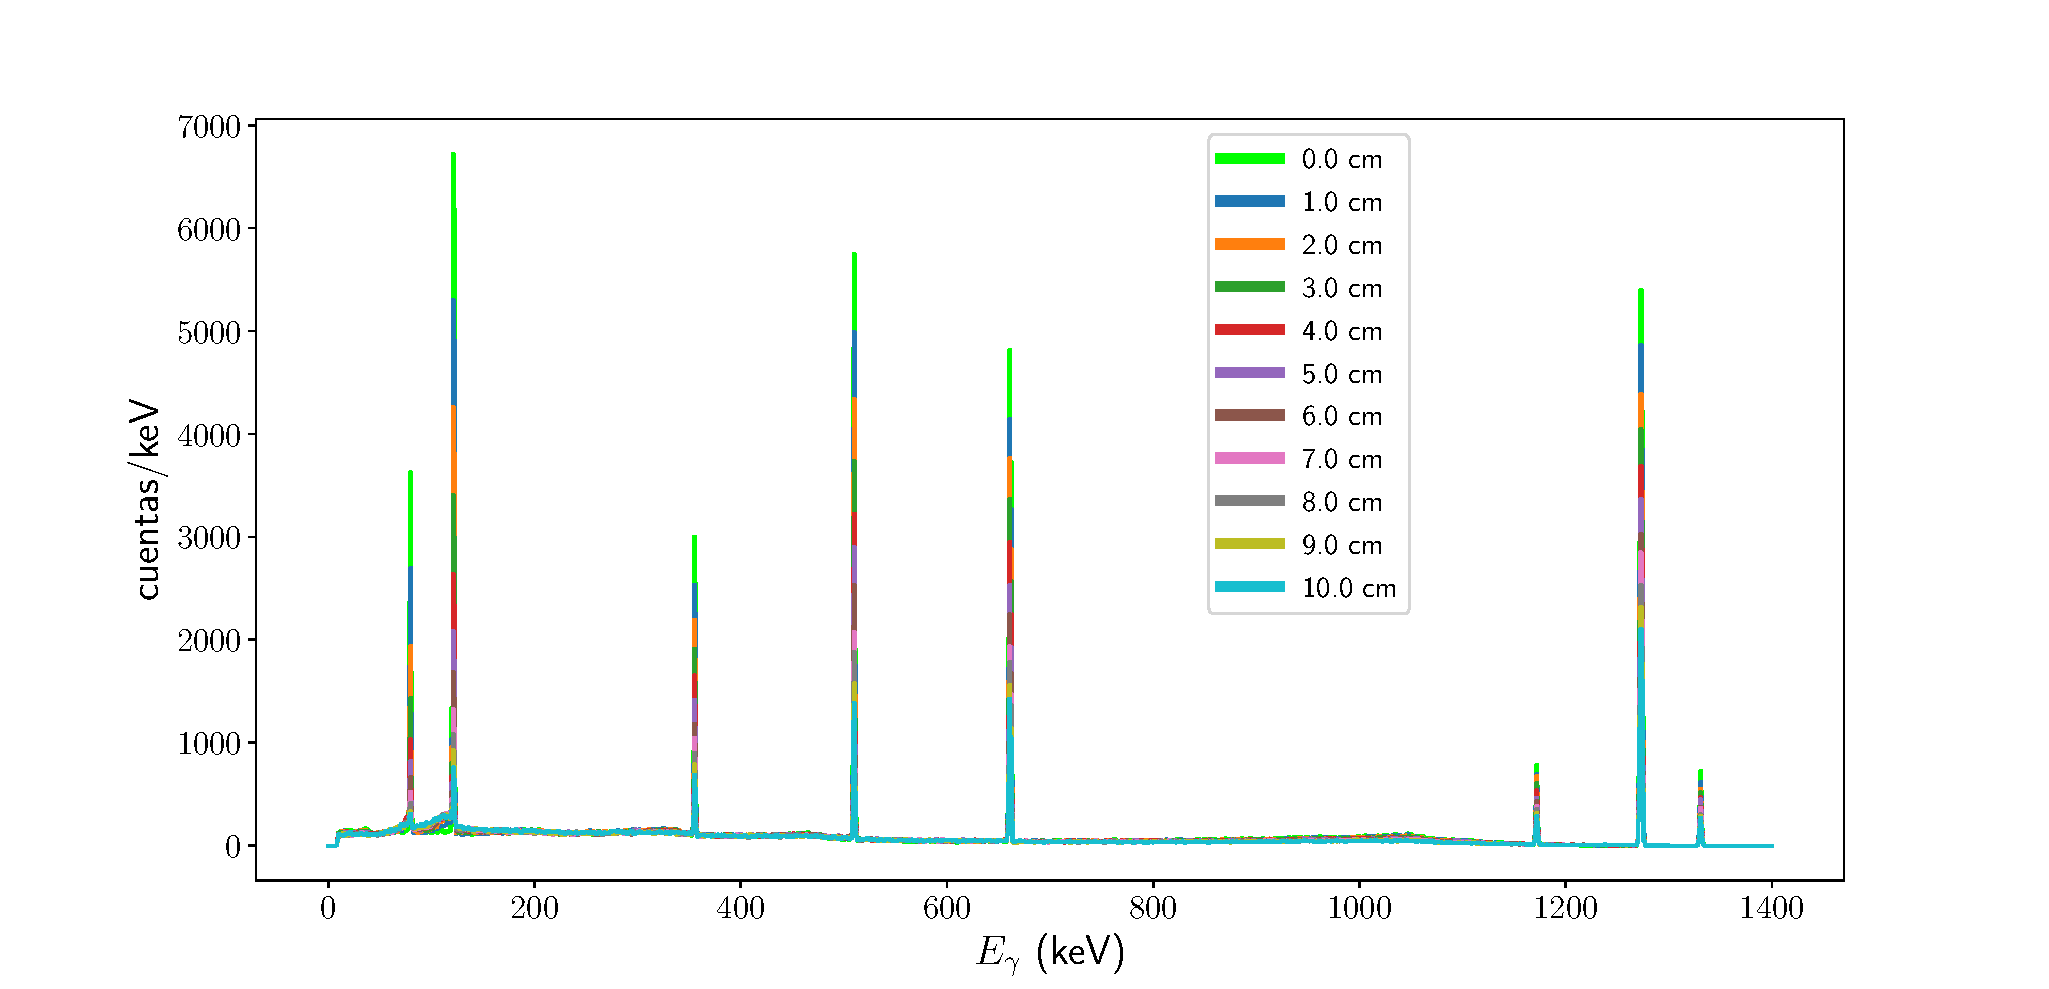
\includegraphics[width=1.0\linewidth]{Kap4/espectro_m1-10M-trans.pdf}
	\caption{Espectro de 10 láminas de Morteros1. Transmisión}
	\label{fig:espectrom1-10m-trans}
\end{figure}


Como se puede ver, cuanto mas grueso el material, la intensidad máxima disminuye. Esto se debe a que obedece la ecuación \ref{intensidad}. 

\begin{equation}\label{intensidad}
	I=I_0e^{-\mu x}
\end{equation}

donde $I_0$ es la intensidad inicial, $\mu$ el coeficiente de atenuación y $x$ el grosor del material. Esta ultima es la variable, en el presente texto será llamada $t$. El valor de $\mu$ es encontrado para cada fotopico. Es fácil ver que se tendrán 8 valores. Con estos se hace un ajuste de la forma:

\begin{equation}
	\frac{\mu}{\rho}=\alpha\times E^{-n}.
\end{equation}

\begin{figure}[H]
	\centering
	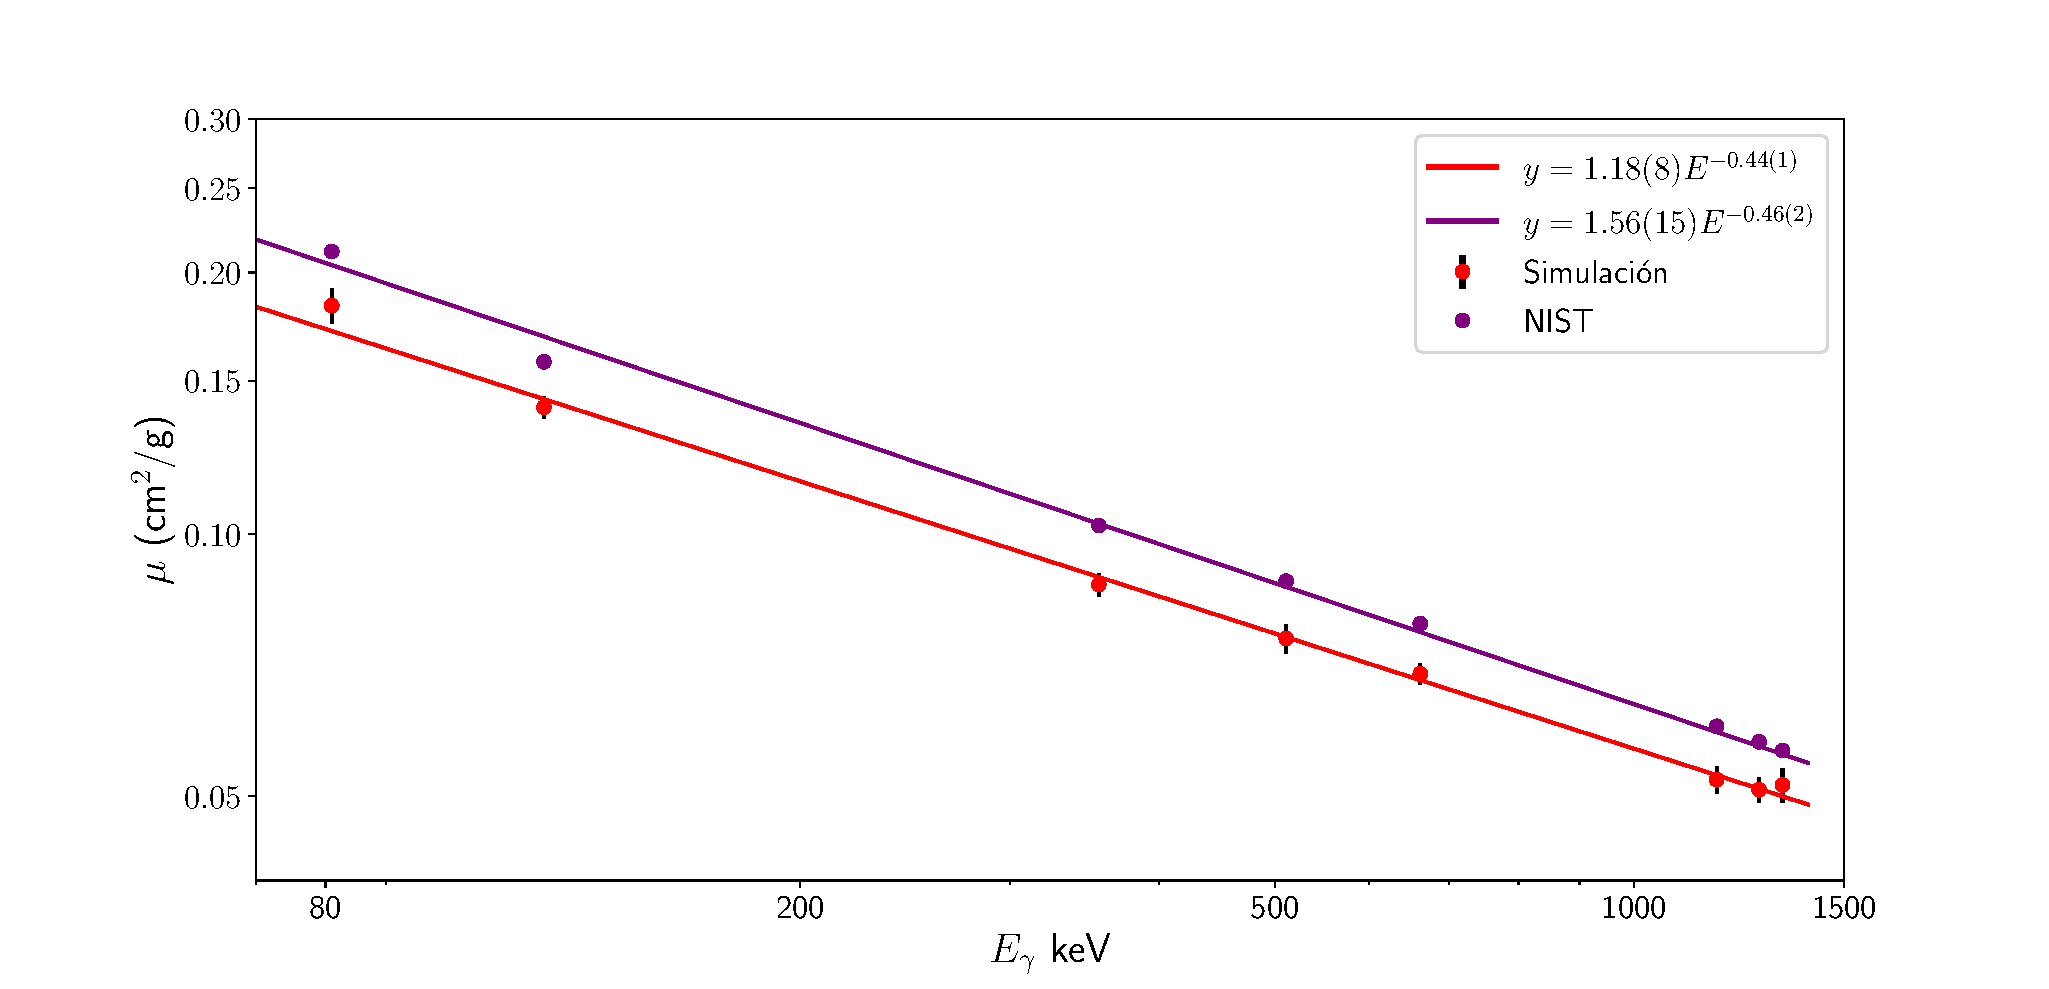
\includegraphics[width=1.0\linewidth]{Kap4/mu-trans-m1.pdf}
	\caption{Ajuste para encontrar $\alpha$ y $n$ a partir de los diferentes $\mu$/$\rho$. Morteros1.}
	\label{fig:mu-trans-m1}
\end{figure}

En la figura anterior podemos ver los valores de interés con su respectiva incertidumbre. Es importante mencionar que allí se grafica el coeficiente de atenuación másico $\mu_T$, el cual fue definido anteriormente. Como se puede observar, los resultados obtenidos con la simulación son similares a los de la base de datos NIST. Por otro lado, la incertidumbre para los datos de NIST esta asociada unicamente al ajuste.

 
\subsection{Retrodispersión.}

\begin{figure}[H]
	\centering
	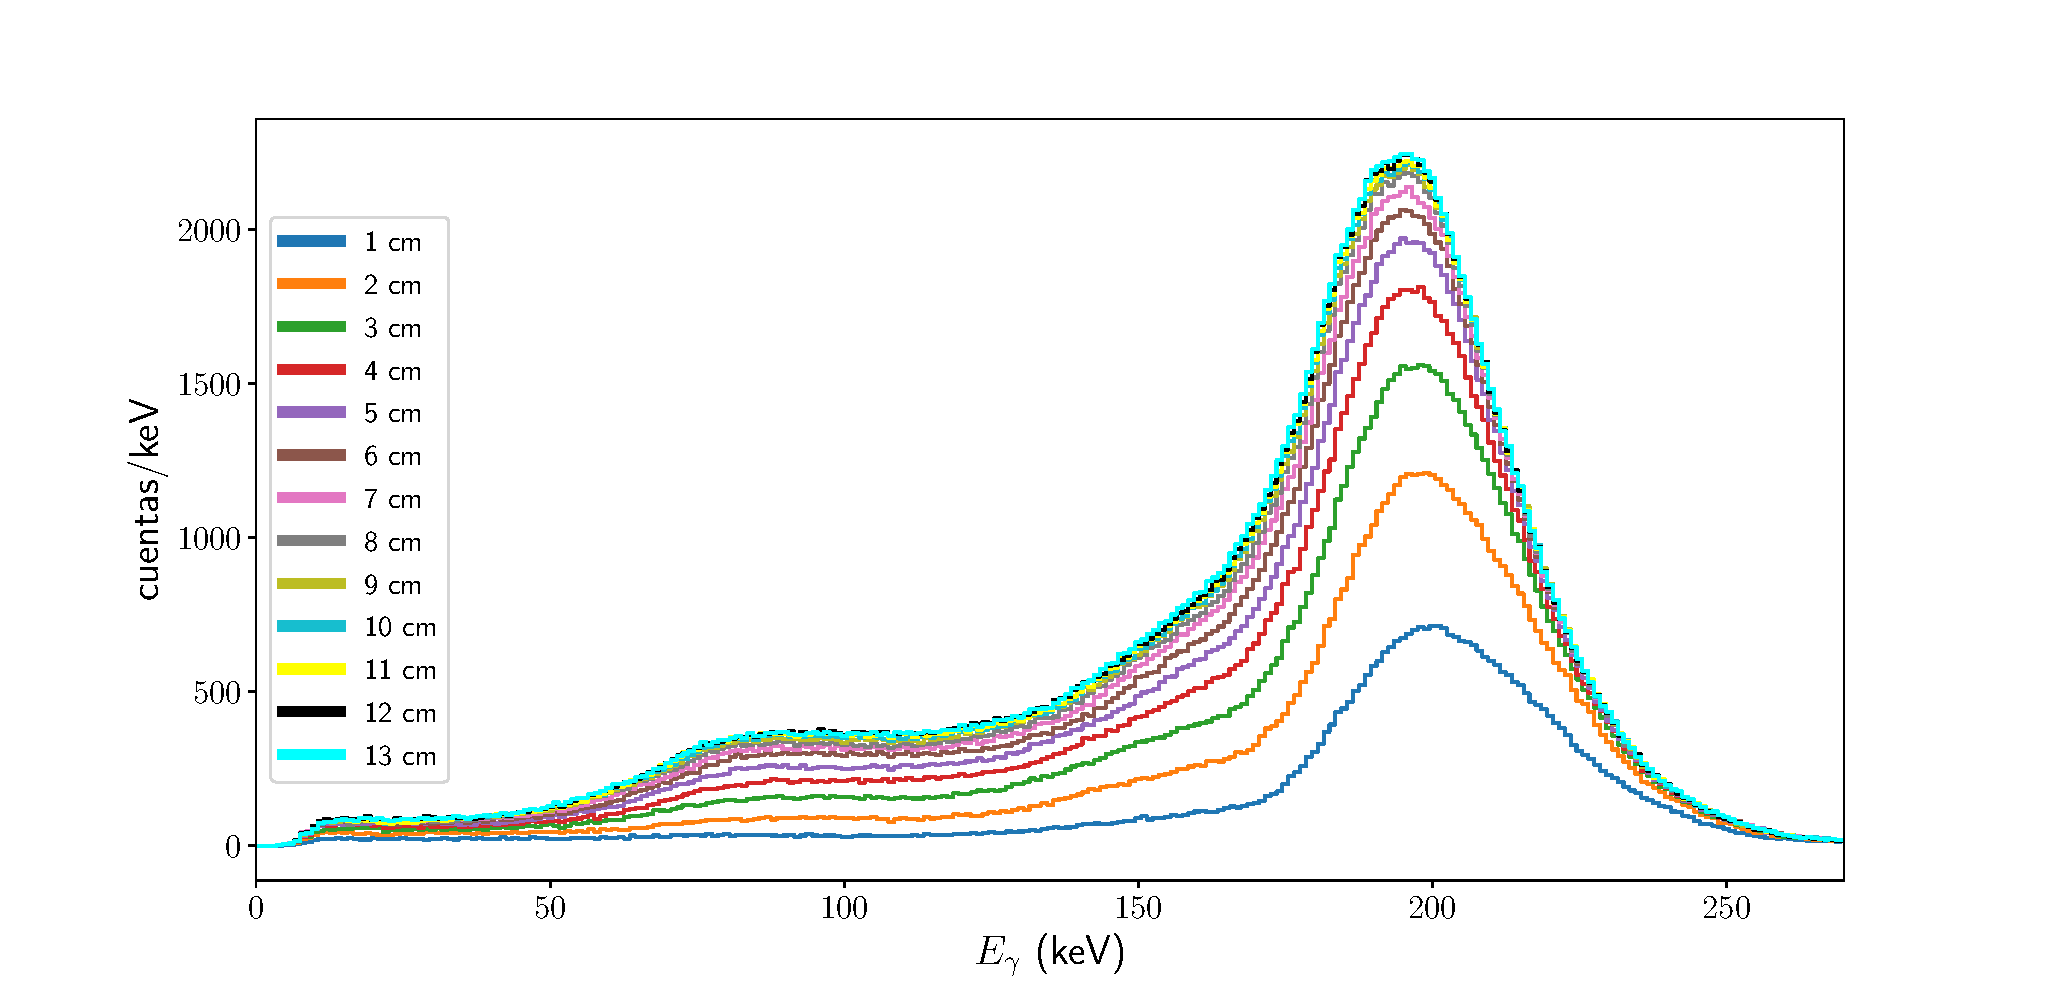
\includegraphics[width=1.0\linewidth]{Kap4/espectros_m1.pdf}
	\caption{Espectro de 10 láminas de Morteros1.}
	\label{fig:espectrosm1}
\end{figure}

En la figura \ref{fig:espectrosm1} se puede apreciar el comportamiento de las intensidades a medida que aumenta el grosor del material. De acuerdo a la figura \ref{g:Montaje-Exp-Retro} los ángulos que abarca la cara del detector mas próxima a las placas son desde $105^\circ$ hasta $164^\circ$, y las energías asociadas son $262$ keV y $197$ keV respectivamente. 
 
\begin{figure}[H]
	\centering
	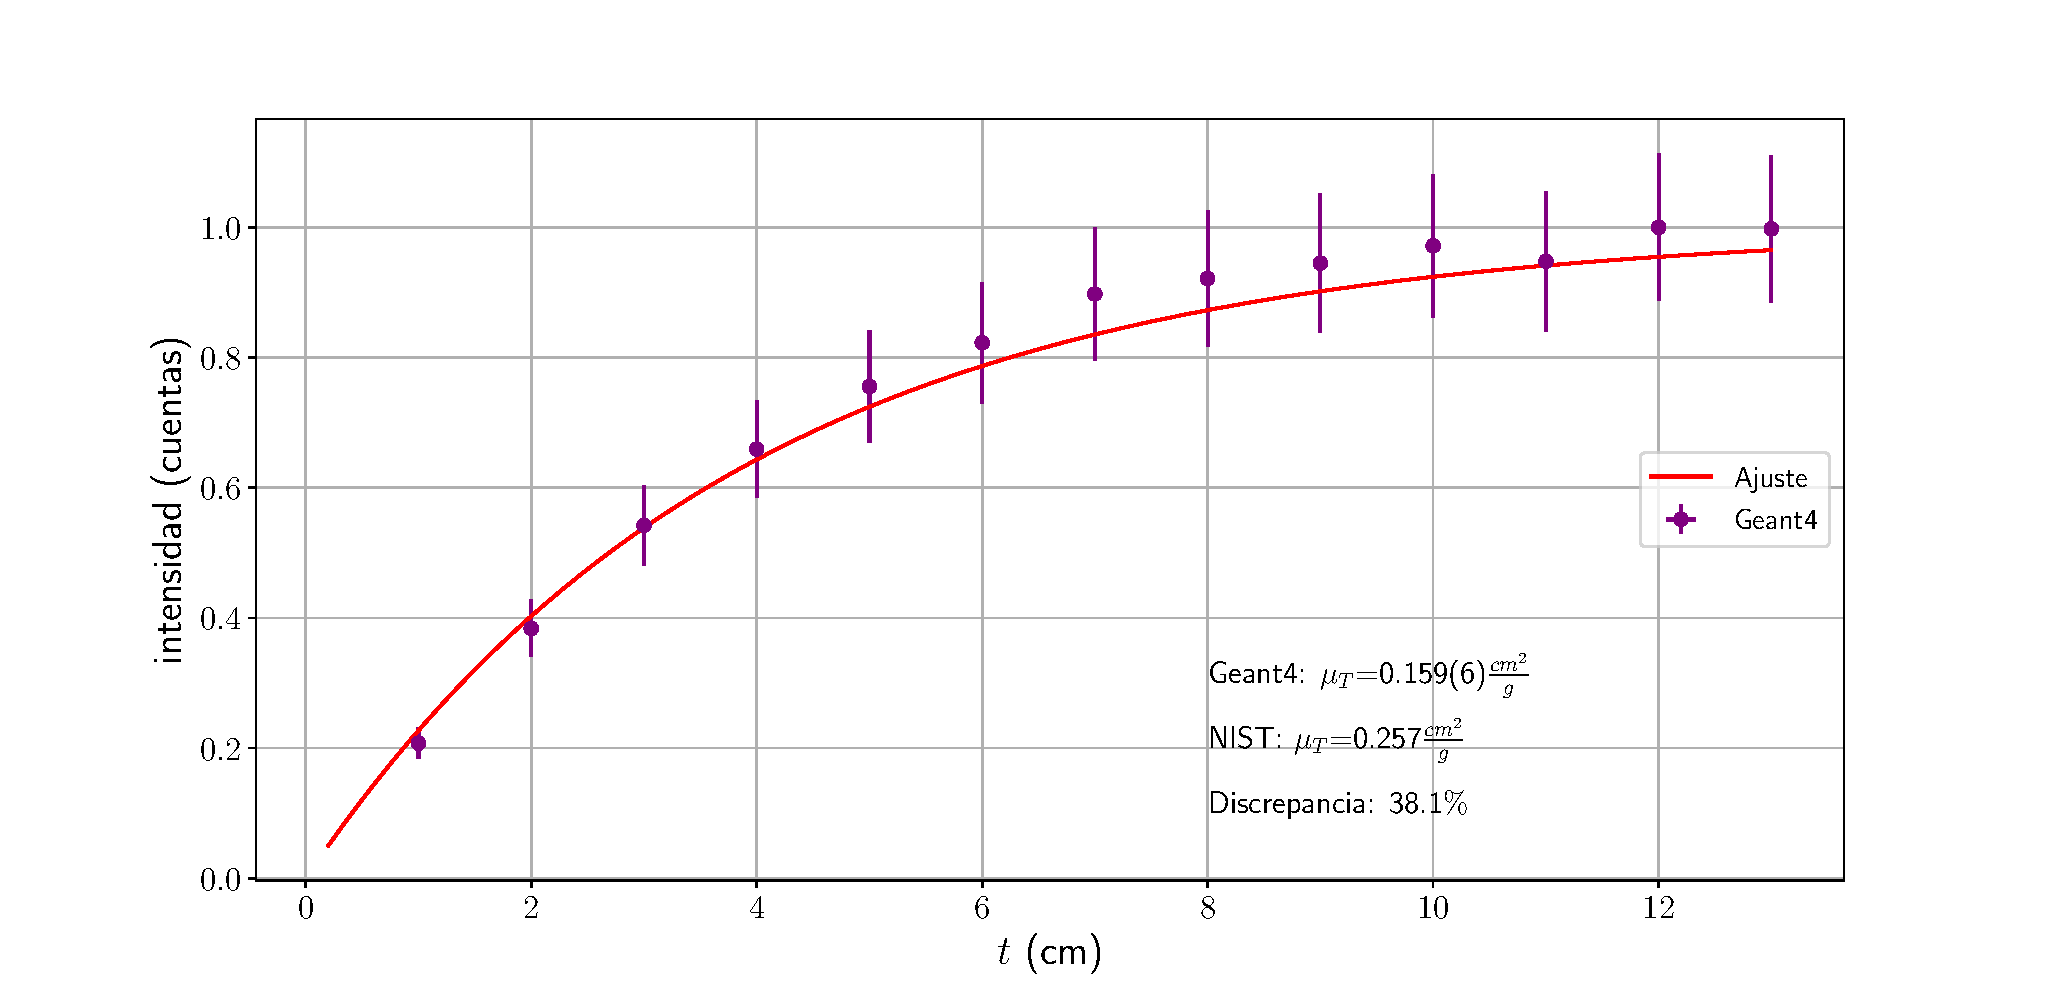
\includegraphics[width=1.0\linewidth]{Kap4/mu_T-m1.pdf}
	\caption{Valores de $\mu_T$ para Morteros 1.}
	\label{fig:mut-m1}
\end{figure}

Una vez encontradas las intensidades asociadas a cada grosor se hace un ajuste tal y como se ve en la figura \ref{fig:mut-m1}. Este ajuste permite encontrar el valor de $\mu_T$, además, de la base de datos NIST se encuentra el valor esta cantidad. Como se puede apreciar, la discrepancia entre estos dos valores es considerable.

 \section{Morteros 2.}
 
 En la tabla \ref{t:medidas-morteros2} se encuentran las dimensiones asociadas a los morteros de este lote. Es importante mencionar que dichos valores son similares con respecto al lote anterior, pues en ambos casos se usaron los mismos recipientes para la construcción.
 
 
 \begin{table}[H]
 	\centering
 	\begin{tabular}{|c|c|c|c|c|c|c|c|}
 		\hline
 		\multicolumn{8}{|c|}{Laminas de Morteros2}                                                                             \\ \hline
 		\multirow{2}{*}{Lamina \#} & Masa {[}g{]} & H1 {[}cm{]} & H2 {[}cm{]} & L1 {[}cm{]} & L2 {[}cm{]} & W1 {[}cm{]} & W2 {[}cm{]} \\ \cline{2-8} 
 		& (+/- 0.01)   & \multicolumn{6}{c|}{(+/- 0.001)}                                                  \\ \hline
 		1                          & 149.35       & 9.760       & 9.706      &9.518         & 9.523      & 0.757       & 0.974       \\ \hline
 		2                          & 157.36       & 9.742       & 9.753      &9.564         & 9.624      & 0.955       & 0.991       \\ \hline
 		3                          & 151.53       & 9.742       & 9.722      &9.615         & 9.493      & 0.923       & 0.956       \\ \hline
 		4                          & 136.97       & 9.757       & 9.794      &9.577         & 9.528      & 0.871       & 0.921       \\ \hline
 	\end{tabular}
 	\caption{Medidas experimentales del lote morteros2.}
 	\label{t:medidas-morteros2}
 \end{table}
 
 En la tabla \ref{t:materiales-mor2} se observa la composición.
 
 \begin{table}[H]
 	\centering
 	\begin{tabular}{|c|c|c|}
 		\hline
 		\multirow{2}{*}{Material} & \multicolumn{2}{c|}{4 placas} \\ \cline{2-3}
 		& g         	& \%        	\\ \hline
 		Cemento Portland      	& 160      	& 22.535    	\\ \hline
 		Arena Peña         	& 450      	& 63.380    	\\ \hline
 		Agua                  	& 100     	& 14.084     	\\ \hline
 	\end{tabular}
 	\caption{Proporción porcentual en la elaboración de morteros2.}
 	\label{t:materiales-morteros2}
 \end{table}
 
 Se evidencia que la densidad no cambia mucho respecto al anterior lote, esto se debe a que la composición es similar.
 
 \begin{equation} \label{densidad-mor2}
 \rho=\frac{masa}{volumen}=1.75(5) g/cm^3
 \end{equation}
 
 \subsection{Transmisión.}
 
\begin{figure}[H]
	\centering
	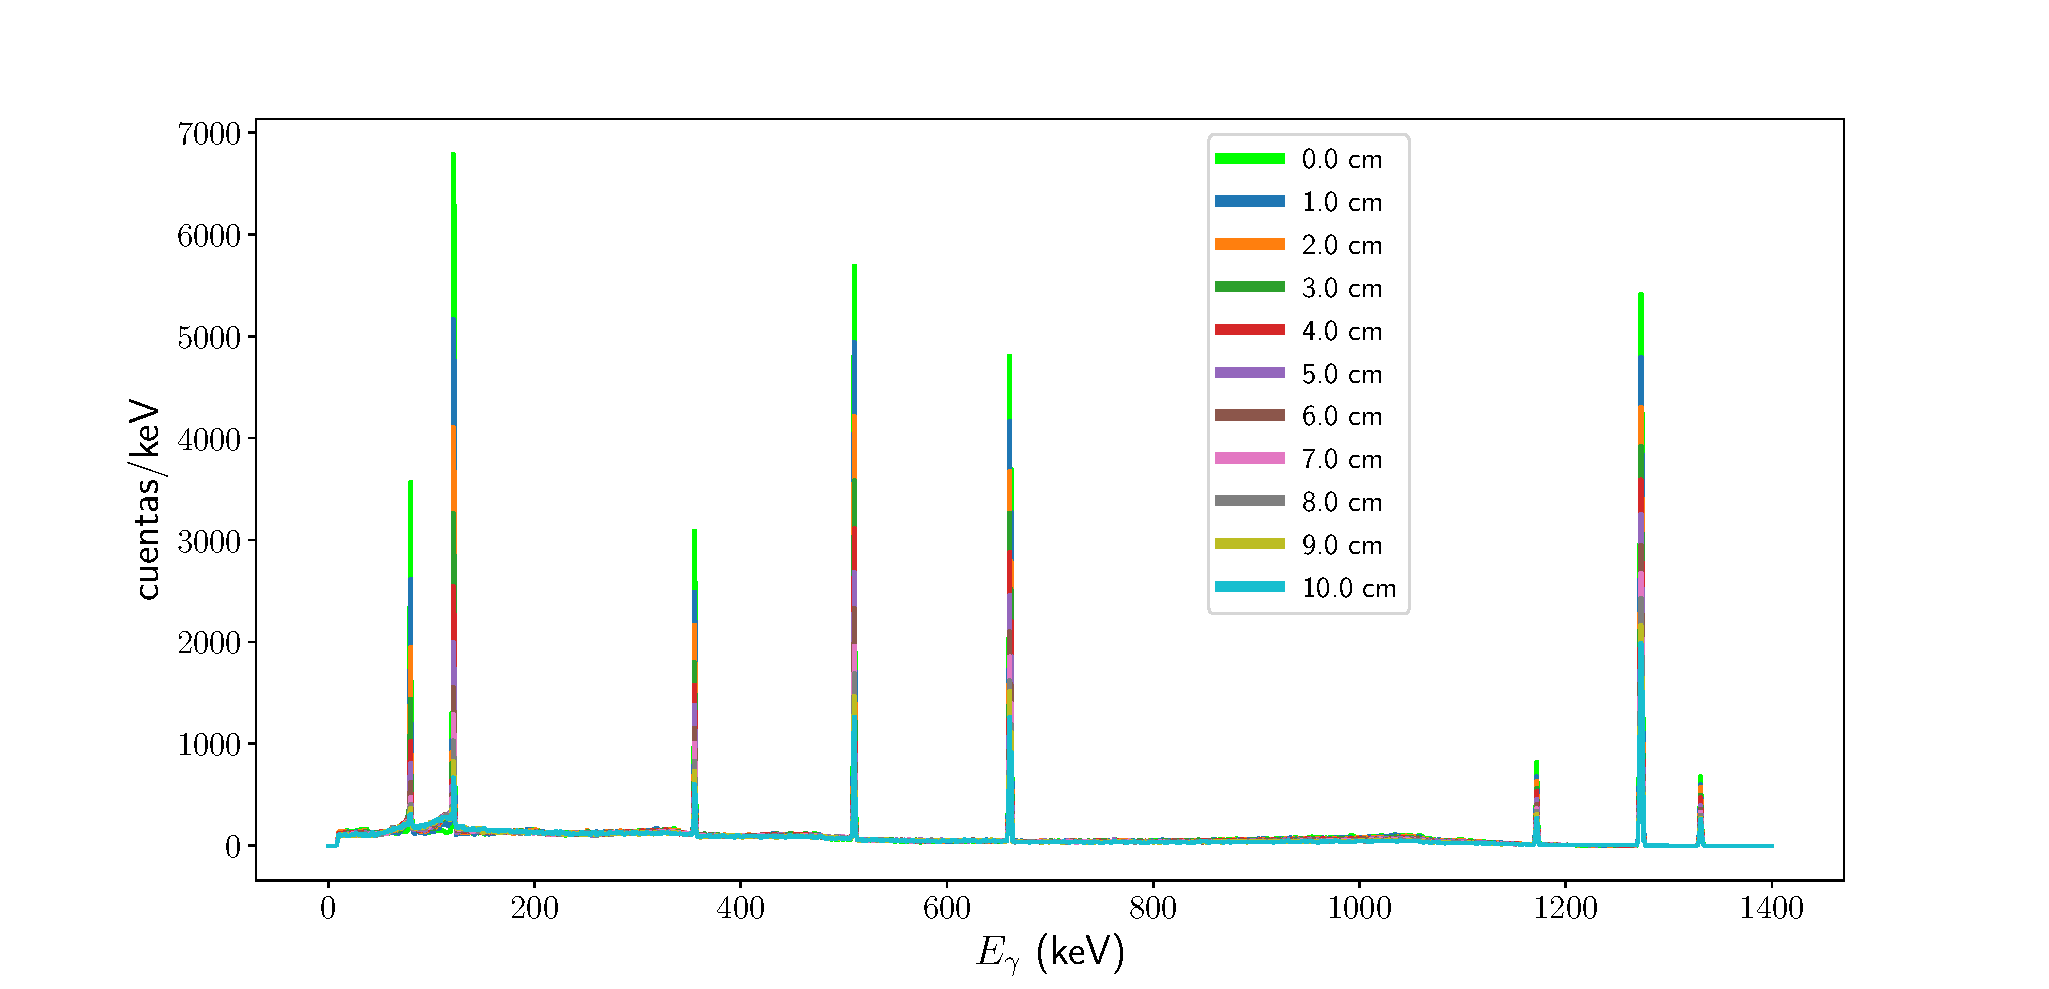
\includegraphics[width=1.0\linewidth]{Kap4/espectro_m2-10M-trans.pdf}
	\caption{Espectro de 10 láminas de Morteros2. Transmisión.}
	\label{fig:espectrom2-10m-trans}
\end{figure}
 
 
\begin{figure}[H]
	\centering
	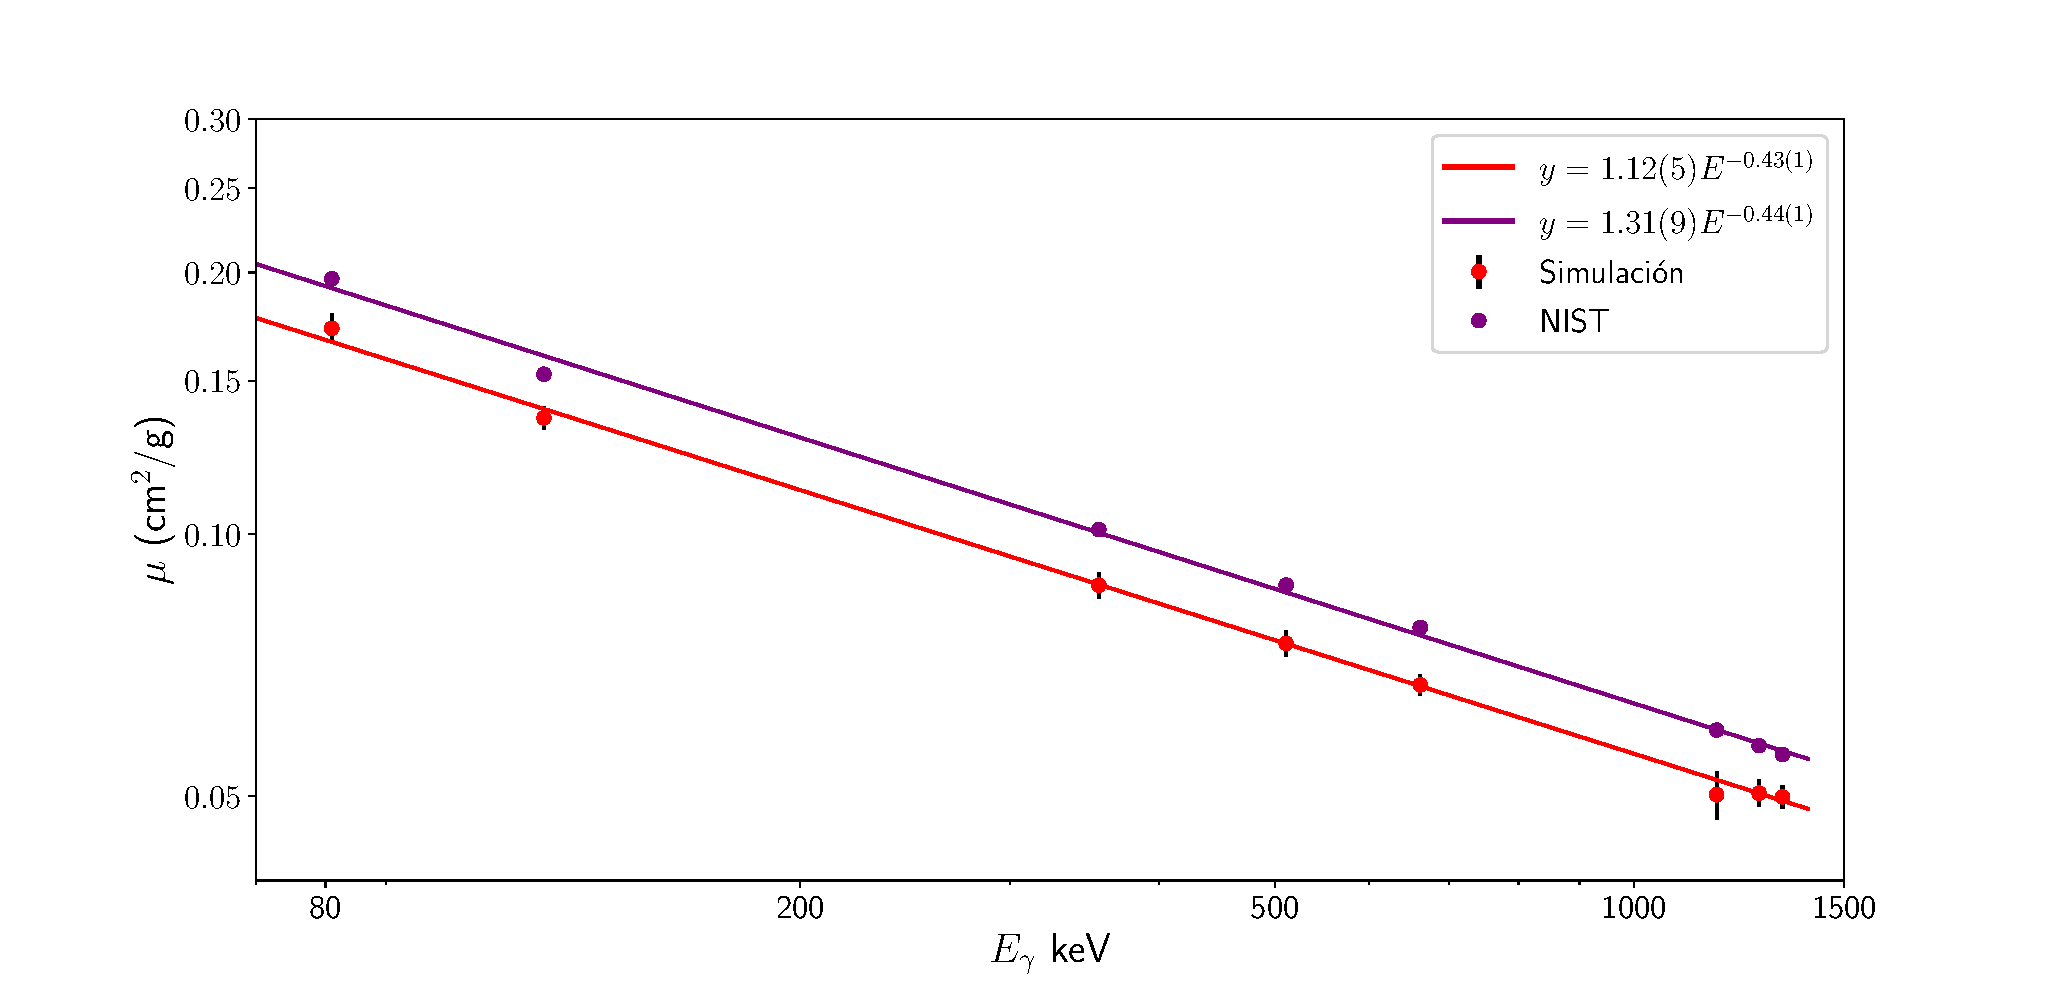
\includegraphics[width=1.0\linewidth]{Kap4/mu-trans-m2.pdf}
	\caption{Ajuste para encontrar $\alpha$ y $n$ a partir de los diferentes $\mu$/$\rho$. Morteros2.}
	\label{fig:mu-trans-m2}
\end{figure}
 
 
 \subsection{Retrodispersión.}
 
 
\begin{figure}[H]
	\centering
	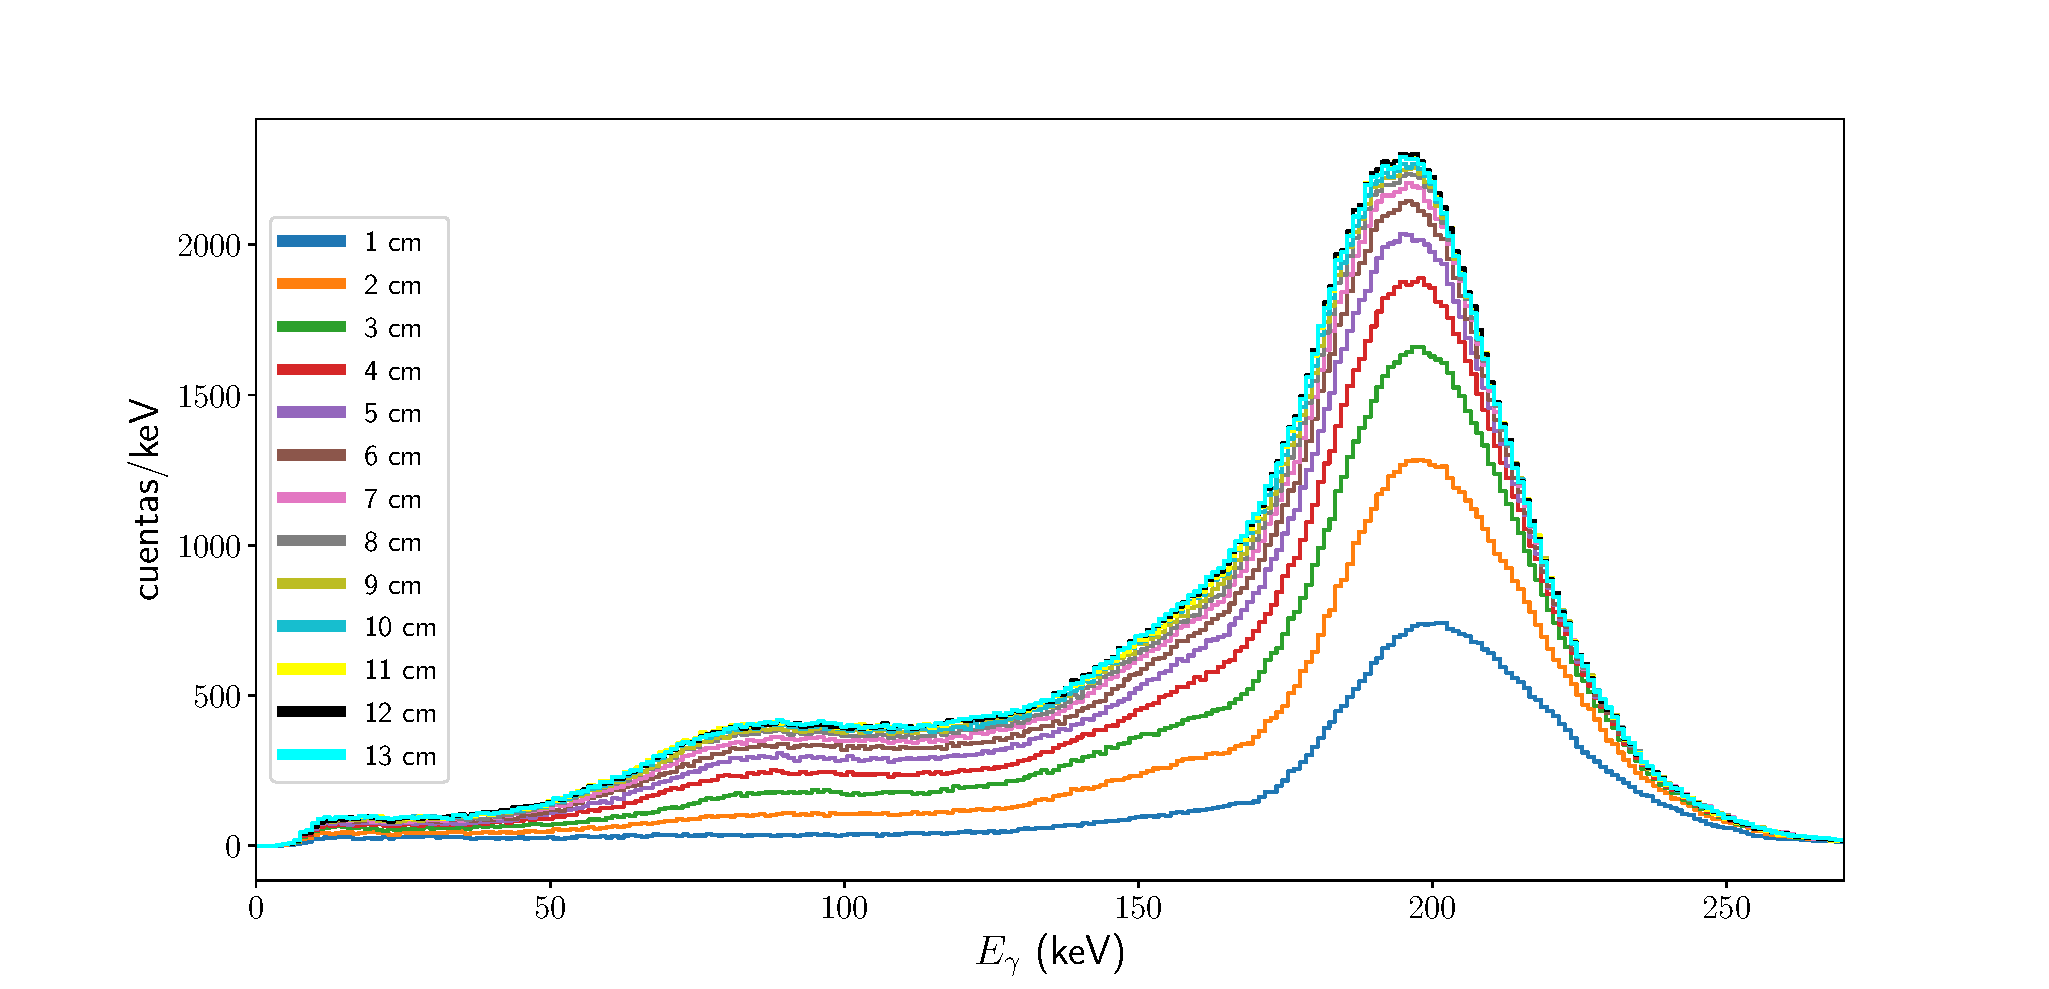
\includegraphics[width=1.0\linewidth]{Kap4/espectro_m2.pdf}
	\caption{Espectro de 10 láminas de Morteros1.}
	\label{fig:espectrom2}
\end{figure}
 
\begin{figure}[H]
	\centering
	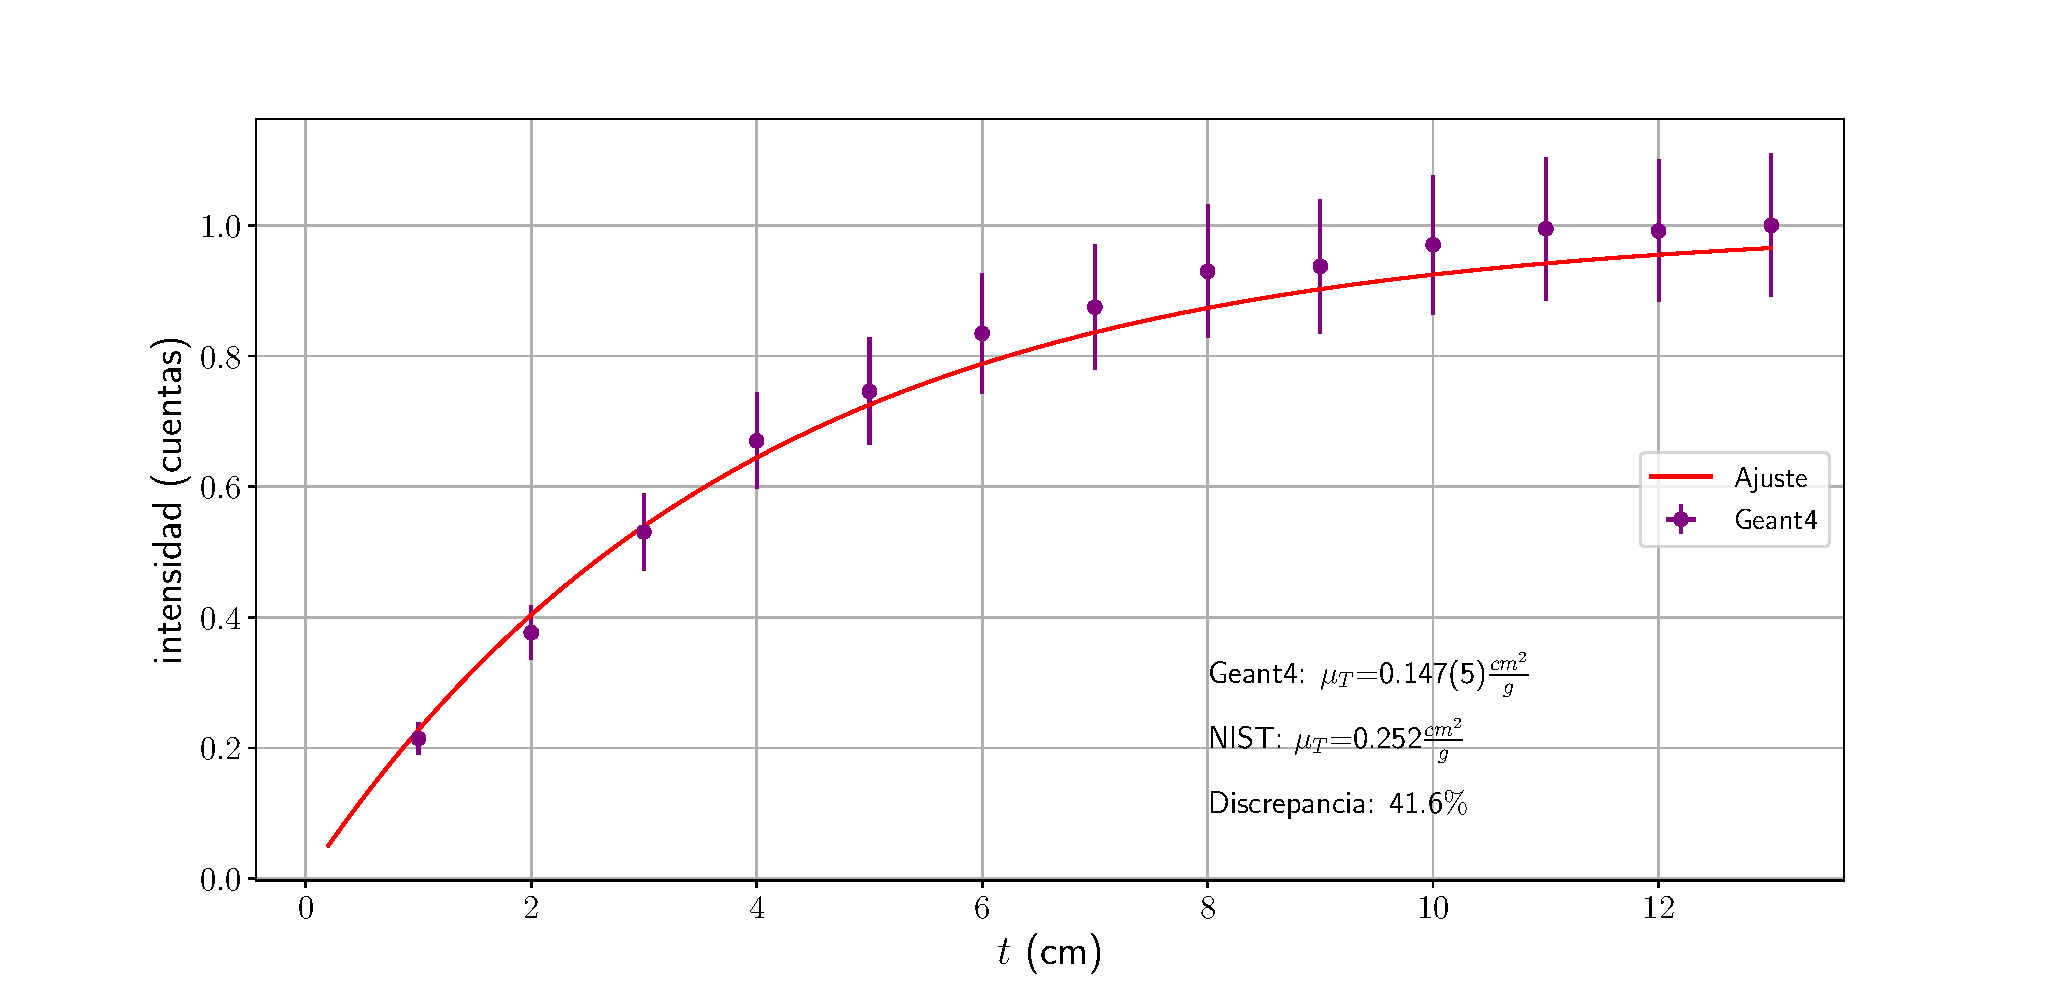
\includegraphics[width=1.0\linewidth]{Kap4/mu_T-m2.pdf}
	\caption{Valores para $\mu_T$. Morteros2.}
	\label{fig:mut-m2}
\end{figure}
 
 
 
 \section{Morteros 3.}
 
  \begin{table}[H]
 	\centering
 	\begin{tabular}{|c|c|c|c|c|c|c|c|}
 		\hline
 		\multicolumn{8}{|c|}{Laminas de Morteros3}                                                                             \\ \hline
 		\multirow{2}{*}{Lamina \#} & Masa {[}g{]} & H1 {[}cm{]} & H2 {[}cm{]} & L1 {[}cm{]} & L2 {[}cm{]} & W1 {[}cm{]} & W2 {[}cm{]} \\ \cline{2-8} 
 		& (+/- 0.01)   & \multicolumn{6}{c|}{(+/- 0.001)}                                                  \\ \hline
 		1                          & 148.71       & 9.825        & 9.820      & 9.583         & 9.712      & 0.975       & 0.935       \\ \hline
 		2                          & 150.32       & 9.672        & 9.616      & 9.528         & 9.577      & 0.968       & 0.929       \\ \hline
 		3                          & 139.83       & 9.613        & 9.640      & 9.463         & 9.521      & 0.949       & 0.916       \\ \hline
 		4                          & 133.72       & 9.864        & 9.839      & 9.526         & 9.550      & 0.852       & 0.916       \\ \hline
 	\end{tabular}
 	\caption{Medidas experimentales del lote morteros2.}
 	\label{t:medidas-morteros3}
 \end{table}
 
 
 \begin{table}[H]
 	\centering
 	\begin{tabular}{|c|c|c|}
 		\hline
 		\multirow{2}{*}{Material} & \multicolumn{2}{c|}{4 placas} \\ \cline{2-3}
 		& g         	& \%        	\\ \hline
 		Cemento Portland      	& 110      	& 15.492    	\\ \hline
 		Arena Sílice         	& 500      	& 70.422    	\\ \hline
 		Agua                  	& 100     	& 14.084     	\\ \hline
 	\end{tabular}
 	\caption{Proporción porcentual en la elaboración de morteros2.}
 	\label{t:materiales-morteros3}
 \end{table}
 
 \begin{equation} \label{densidad-mor3}
 \rho=\frac{masa}{volumen}=1.62(7) g/cm^3
 \end{equation}
 
 \subsection{Transmisión.}
 
\begin{figure}[H]
	\centering
	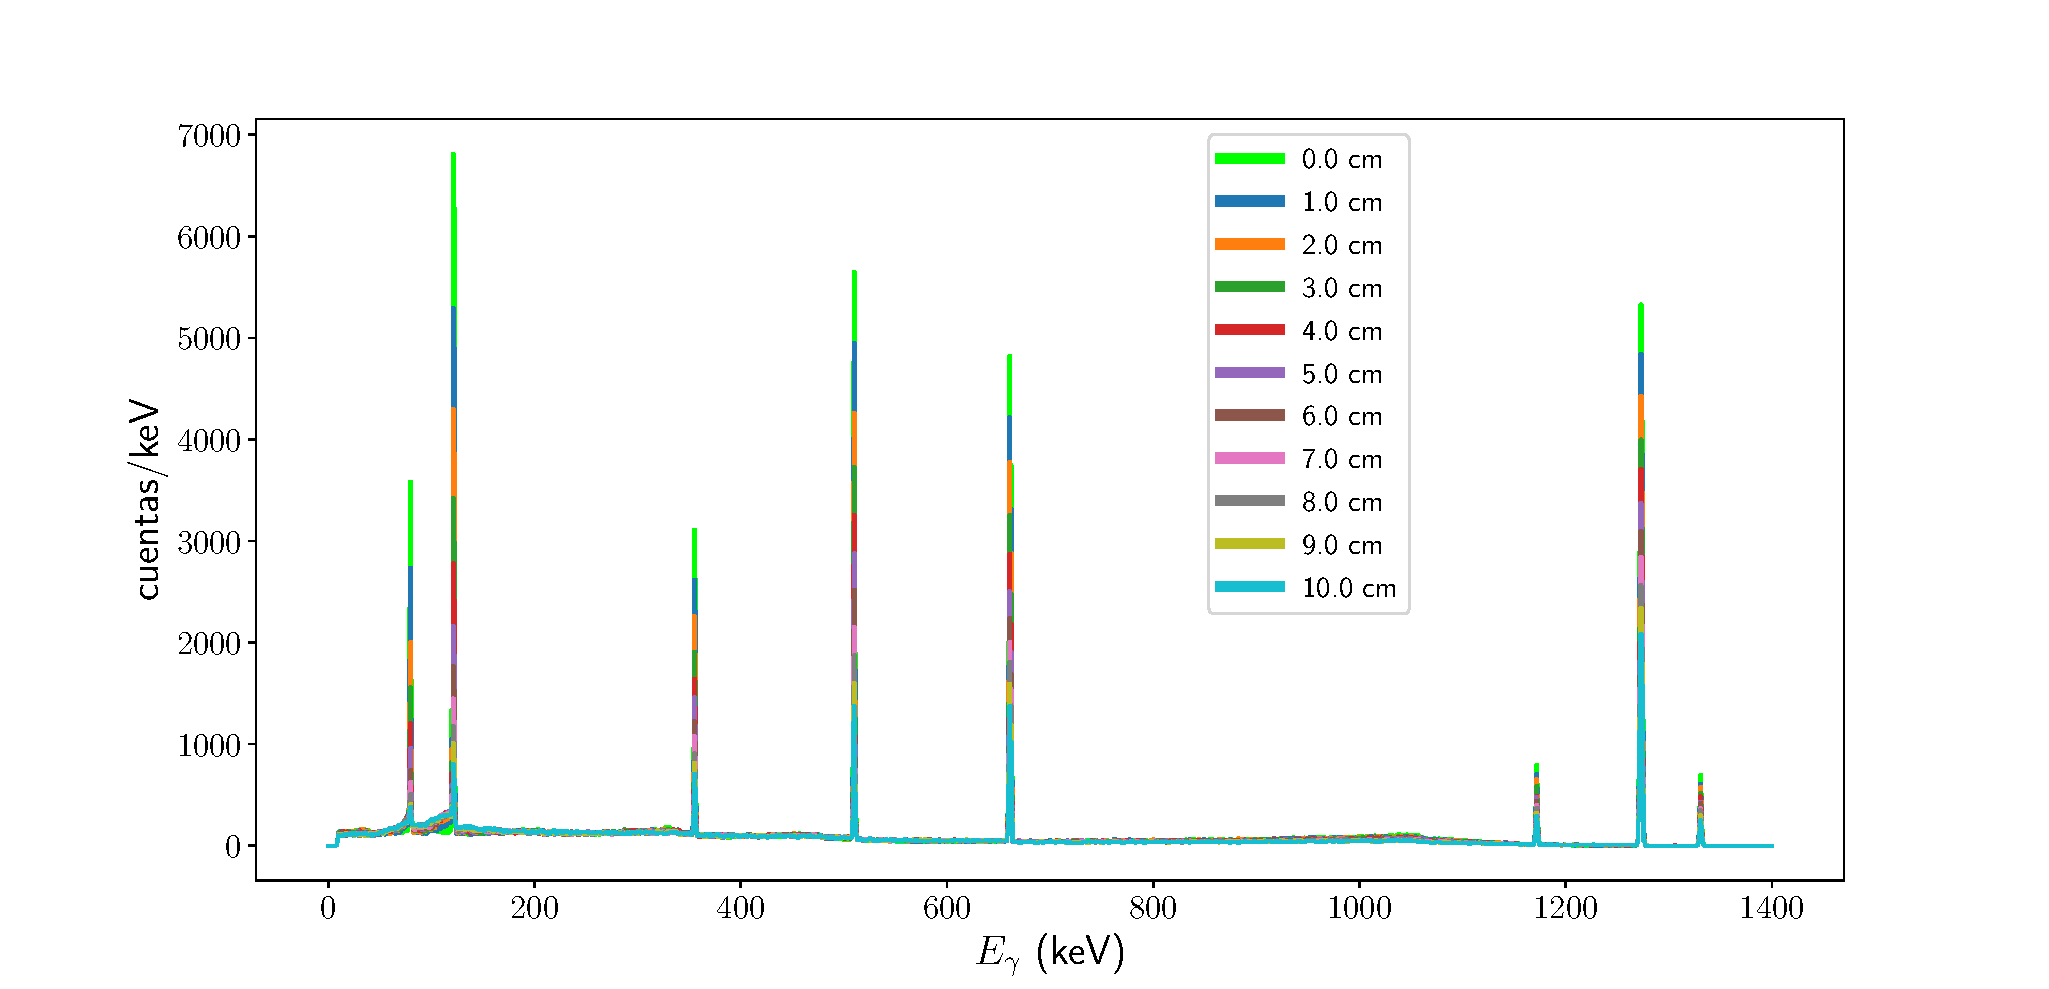
\includegraphics[width=1.0\linewidth]{Kap4/espectro_m3-M10-trans.pdf}
	\caption{Espectro de 10 láminas de Morteros3. Transmisión}
	\label{fig:espectrom3-m10-trans}
\end{figure}
 
\begin{figure}[H]
	\centering
	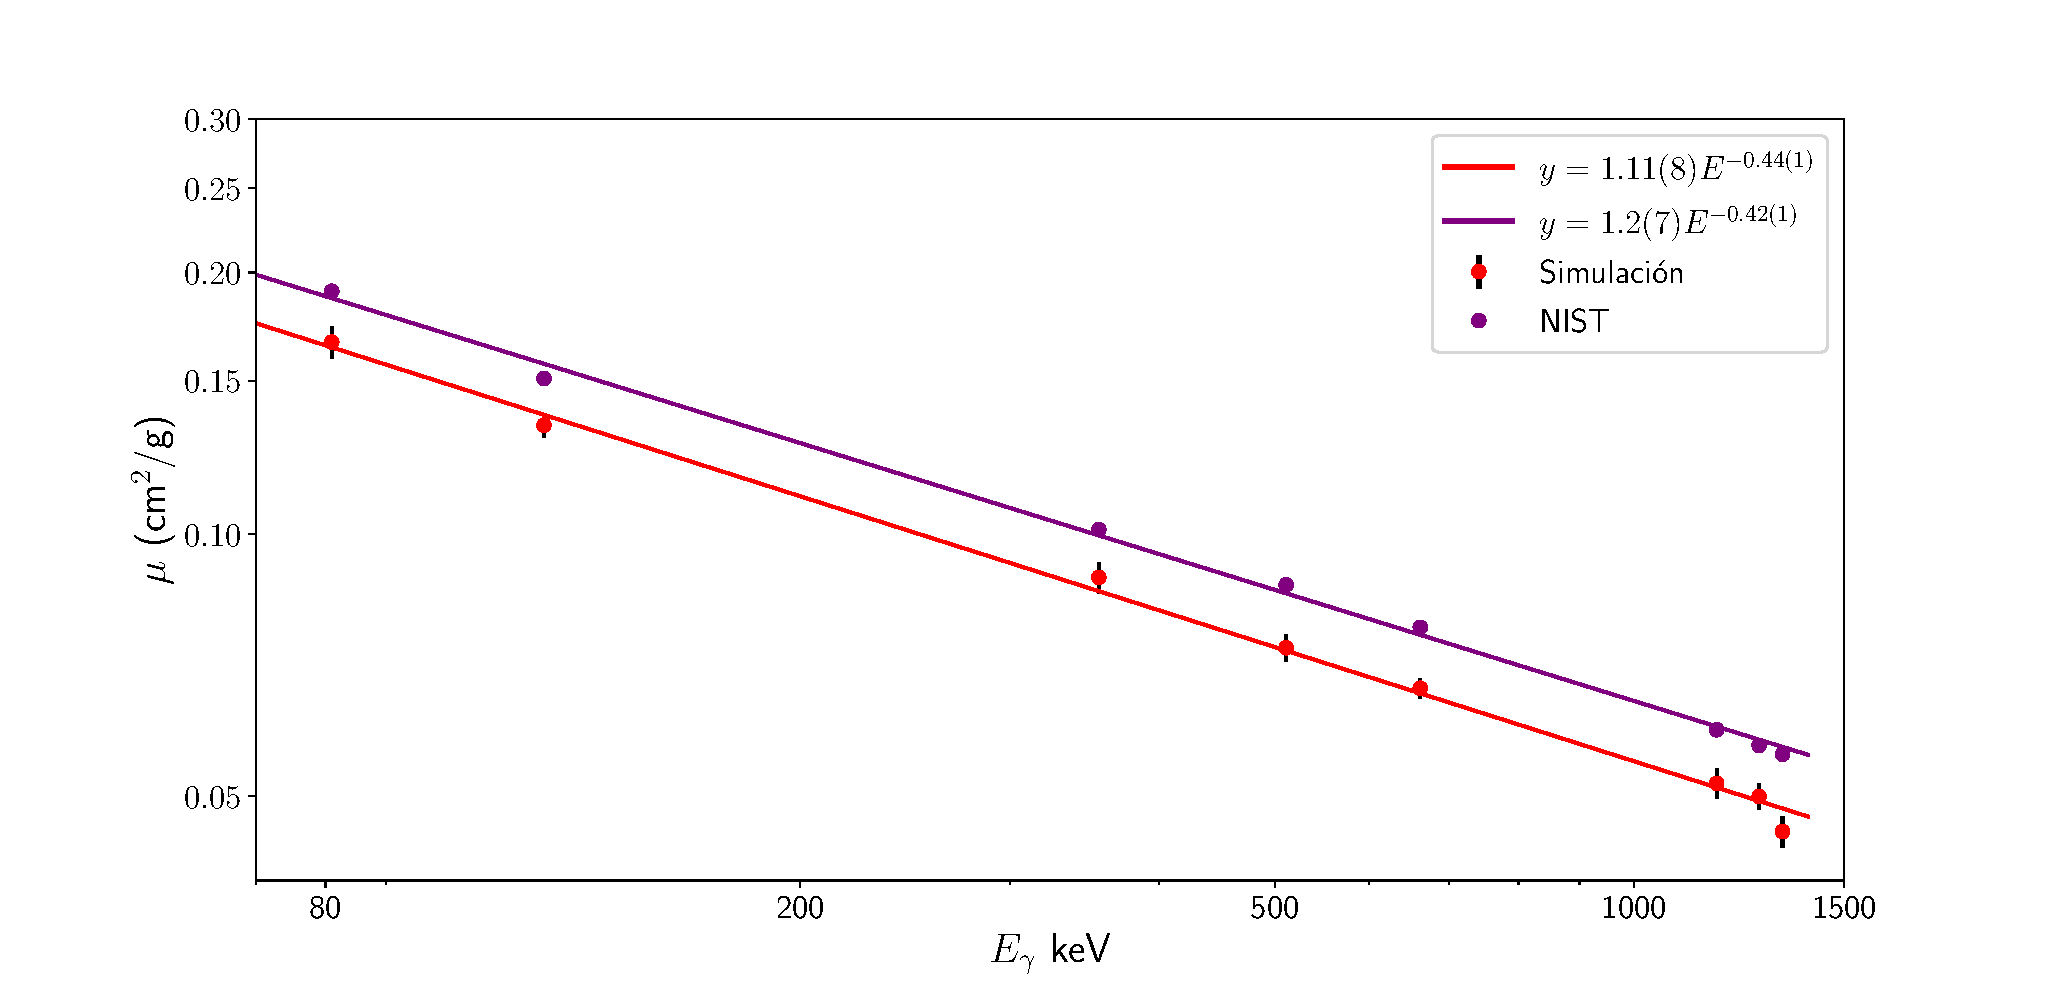
\includegraphics[width=1.0\linewidth]{Kap4/mu-trans-m3.pdf}
	\caption{Ajuste para encontrar $\alpha$ y $n$ a partir de los diferentes $\mu$/$\rho$. Morteros3.}
	\label{fig:mu-trans-m3}
\end{figure}
 
 
 \subsection{Retrodispersión.}
 
\begin{figure}[H]
	\centering
	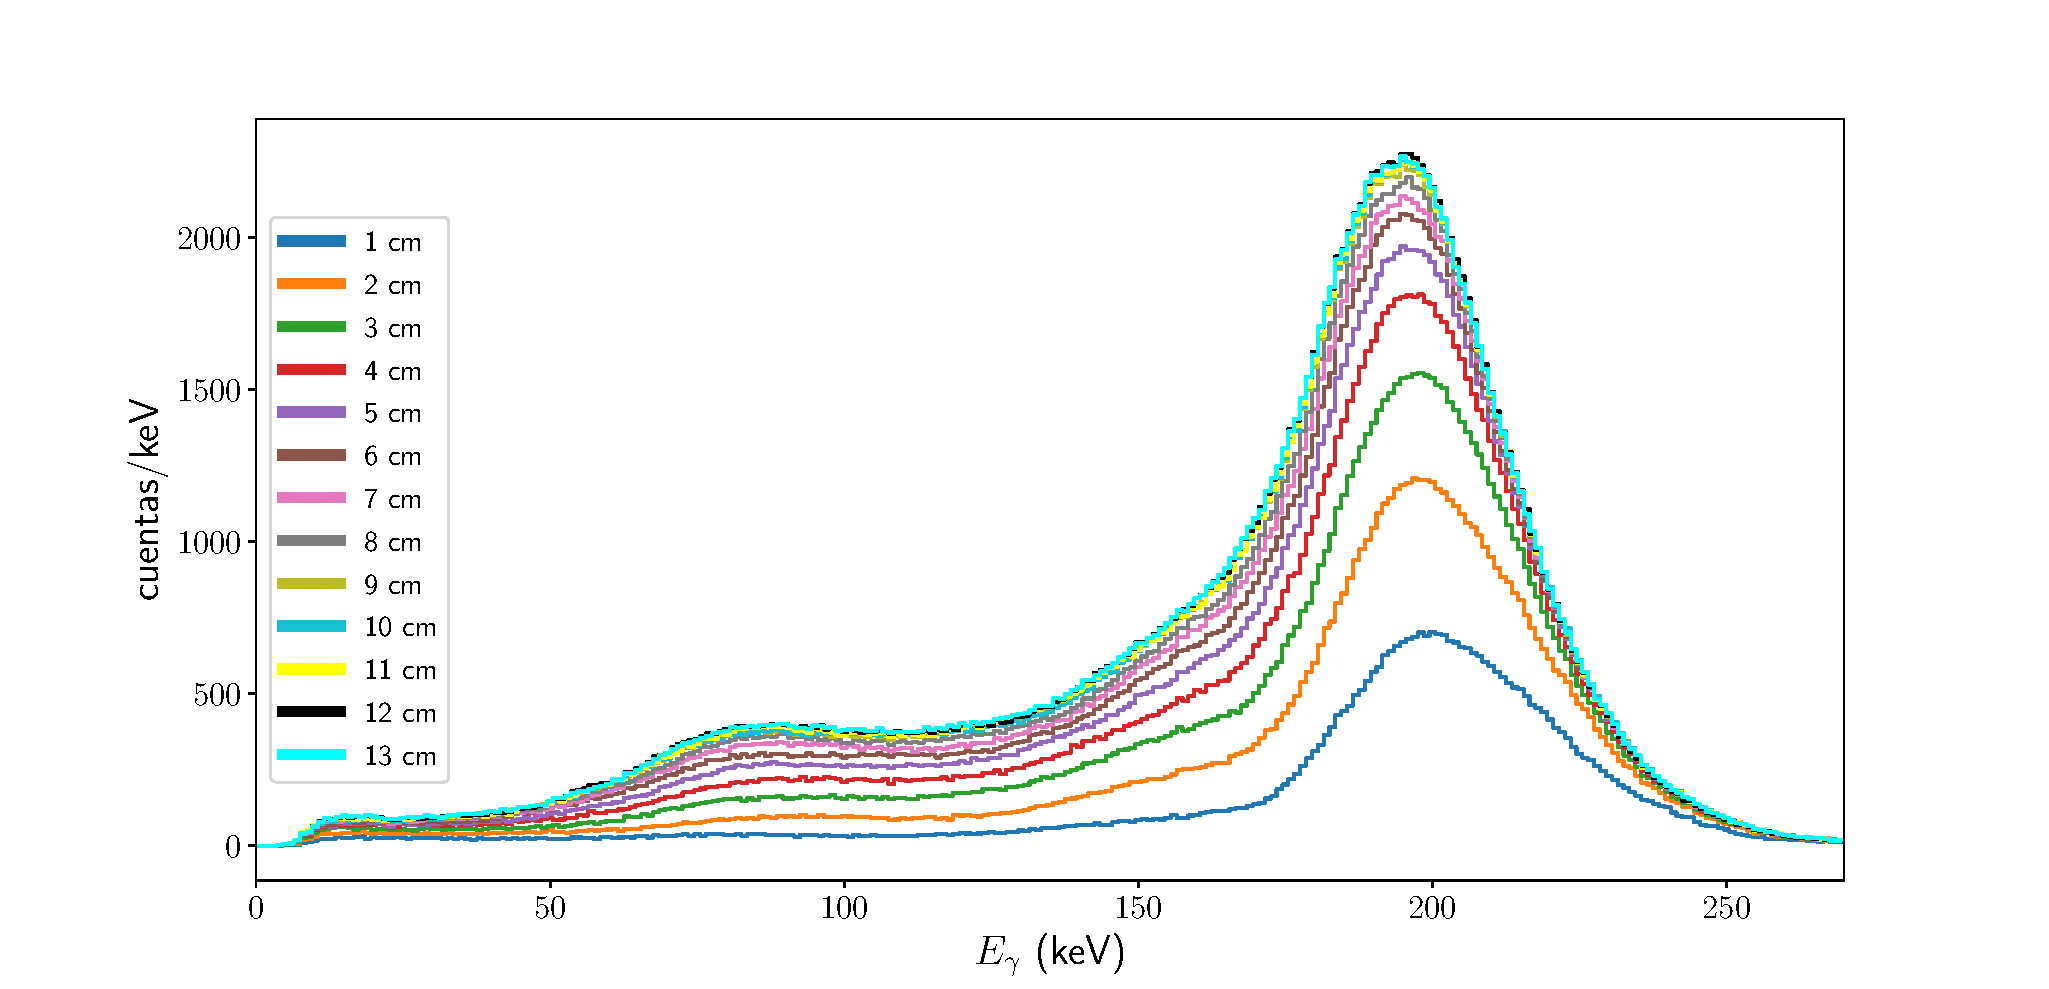
\includegraphics[width=1.0\linewidth]{Kap4/espectro_m3.pdf}
	\caption{Espectro de 10 láminas de Morteros3.}
	\label{fig:espectrom3}
\end{figure}

\begin{figure}[H]
	\centering
	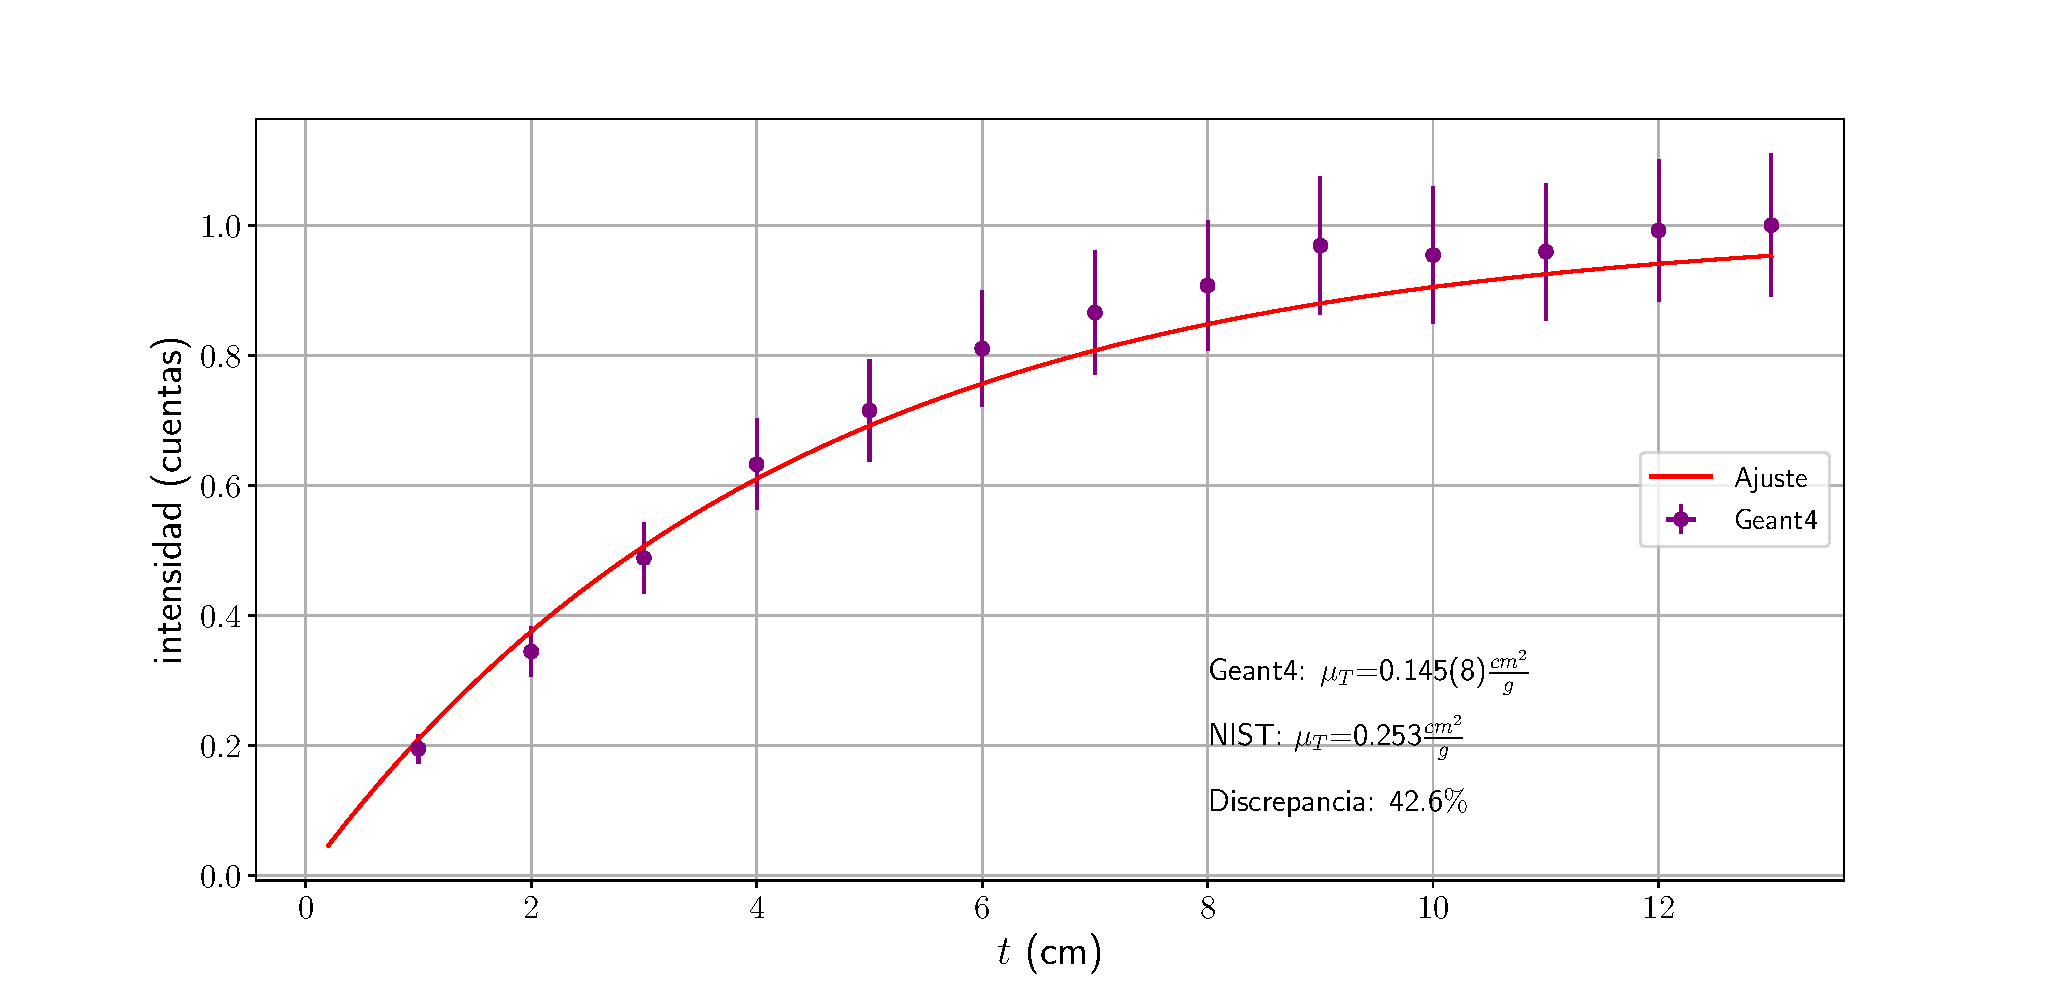
\includegraphics[width=1.0\linewidth]{Kap4/mu_T-m3.pdf}
	\caption{$\mu_T=0.24(1) cm^{-1}$ Morteros3.}
	\label{fig:mut-m3}
\end{figure}

 
 
 
 \section{Morteros 4.}
 
   \begin{table}[H]
 	\centering
 	\begin{tabular}{|c|c|c|c|c|c|c|c|}
 		\hline
 		\multicolumn{8}{|c|}{Laminas de Morteros4}                                                                             \\ \hline
 		\multirow{Lamina \#} & Masa {[}g{]} & H1 {[}cm{]} & H2 {[}cm{]} & L1 {[}cm{]} & L2 {[}cm{]} & W1 {[}cm{]} & W2 {[}cm{]} \\ \cline{2-8} 
 		& (+/- 0.01)   & \multicolumn{6}{c|}{(+/- 0.001)}                                                  \\ \hline
 		1                          & 156.90       & 9.774         & 9.804      & 9.557          & 9.563      & 0.938       & 10.20       \\ \hline
 		2                          & 145.96       & 9.687         & 9.653      & 9.620          & 9.550      & 0.914       & 0.940       \\ \hline
 		3                          & 140.52       & 9.657         & 9.693      & 9.579          & 9.589      & 1.079       & 0.902       \\ \hline
 		4                          & 147.33       & 9.814         & 9.772      & 9.546          & 9.589      & 1.075       & 0.953       \\ \hline
 	\end{tabular}
 	\caption{Medidas experimentales del lote morteros4.}
 	\label{t:medidas-morteros4}
 \end{table}
 
 
 \begin{table}[H]
 	\centering
 	\begin{tabular}{|c|c|c|}
 		\hline
 		\multirow{Material} & \multicolumn{2}{c|}{4 placas} \\ \cline{2-3}
 		& g         	& \%        	\\ \hline
 		Cemento Portland      	& 100      	& 10.989    	\\ \hline
 		Arena Sílice         	& 700      	& 76.923    	\\ \hline
 		Agua                  	& 110     	& 12.087     	\\ \hline
 	\end{tabular}
 	\caption{Proporción porcentual en la elaboración de morteros4.}
 	\label{t:materiales-morteros4}
 \end{table}
 
 \begin{equation} \label{densidad-mor4}
 \rho=\frac{masa}{volumen}=1.62(3) g/cm^3
 \end{equation}
 
 \subsection{Transmisión.}
 
\begin{figure}[H]
	\centering
	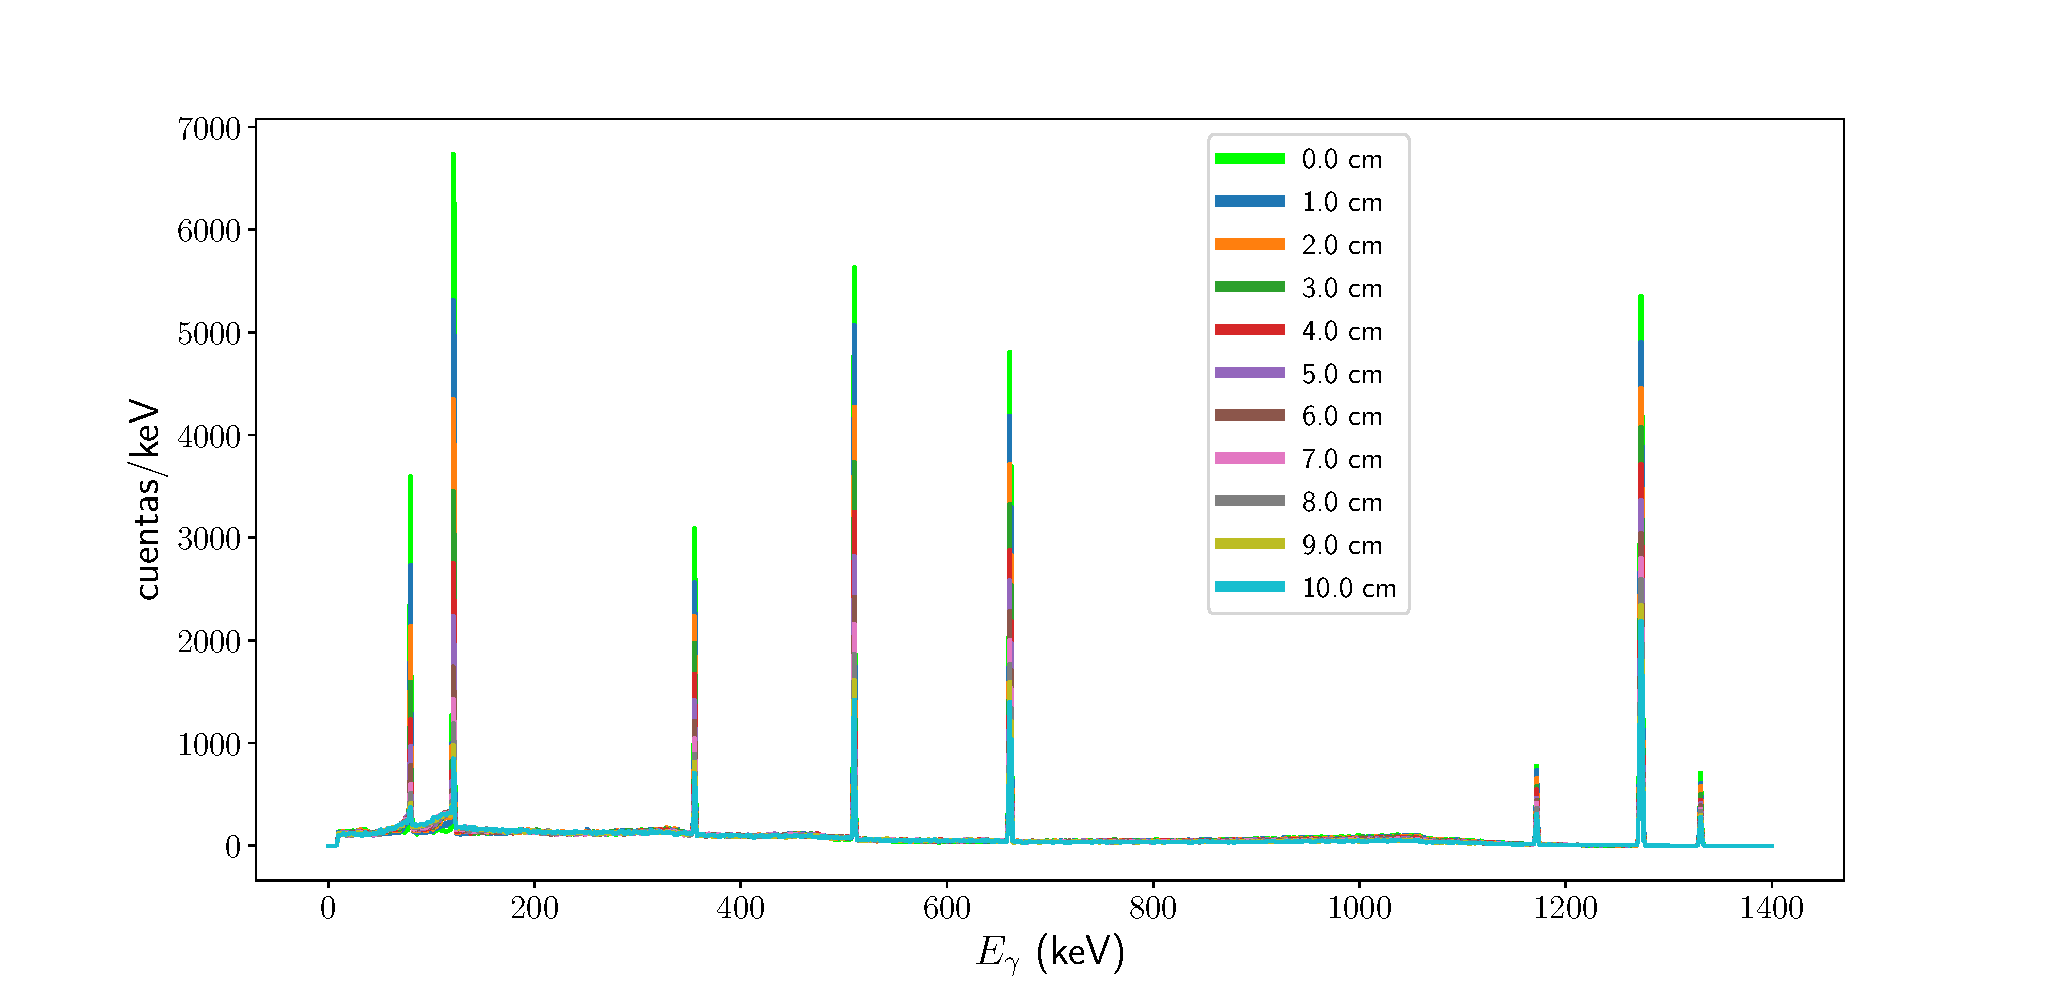
\includegraphics[width=1.0\linewidth]{Kap4/espectro_m4-10M-trans.pdf}
	\caption{Espectro de 10 láminas de Morteros4. Transmisicón}
	\label{fig:espectrom4-10m-trans}
\end{figure}
 
\begin{figure}[H]
	\centering
	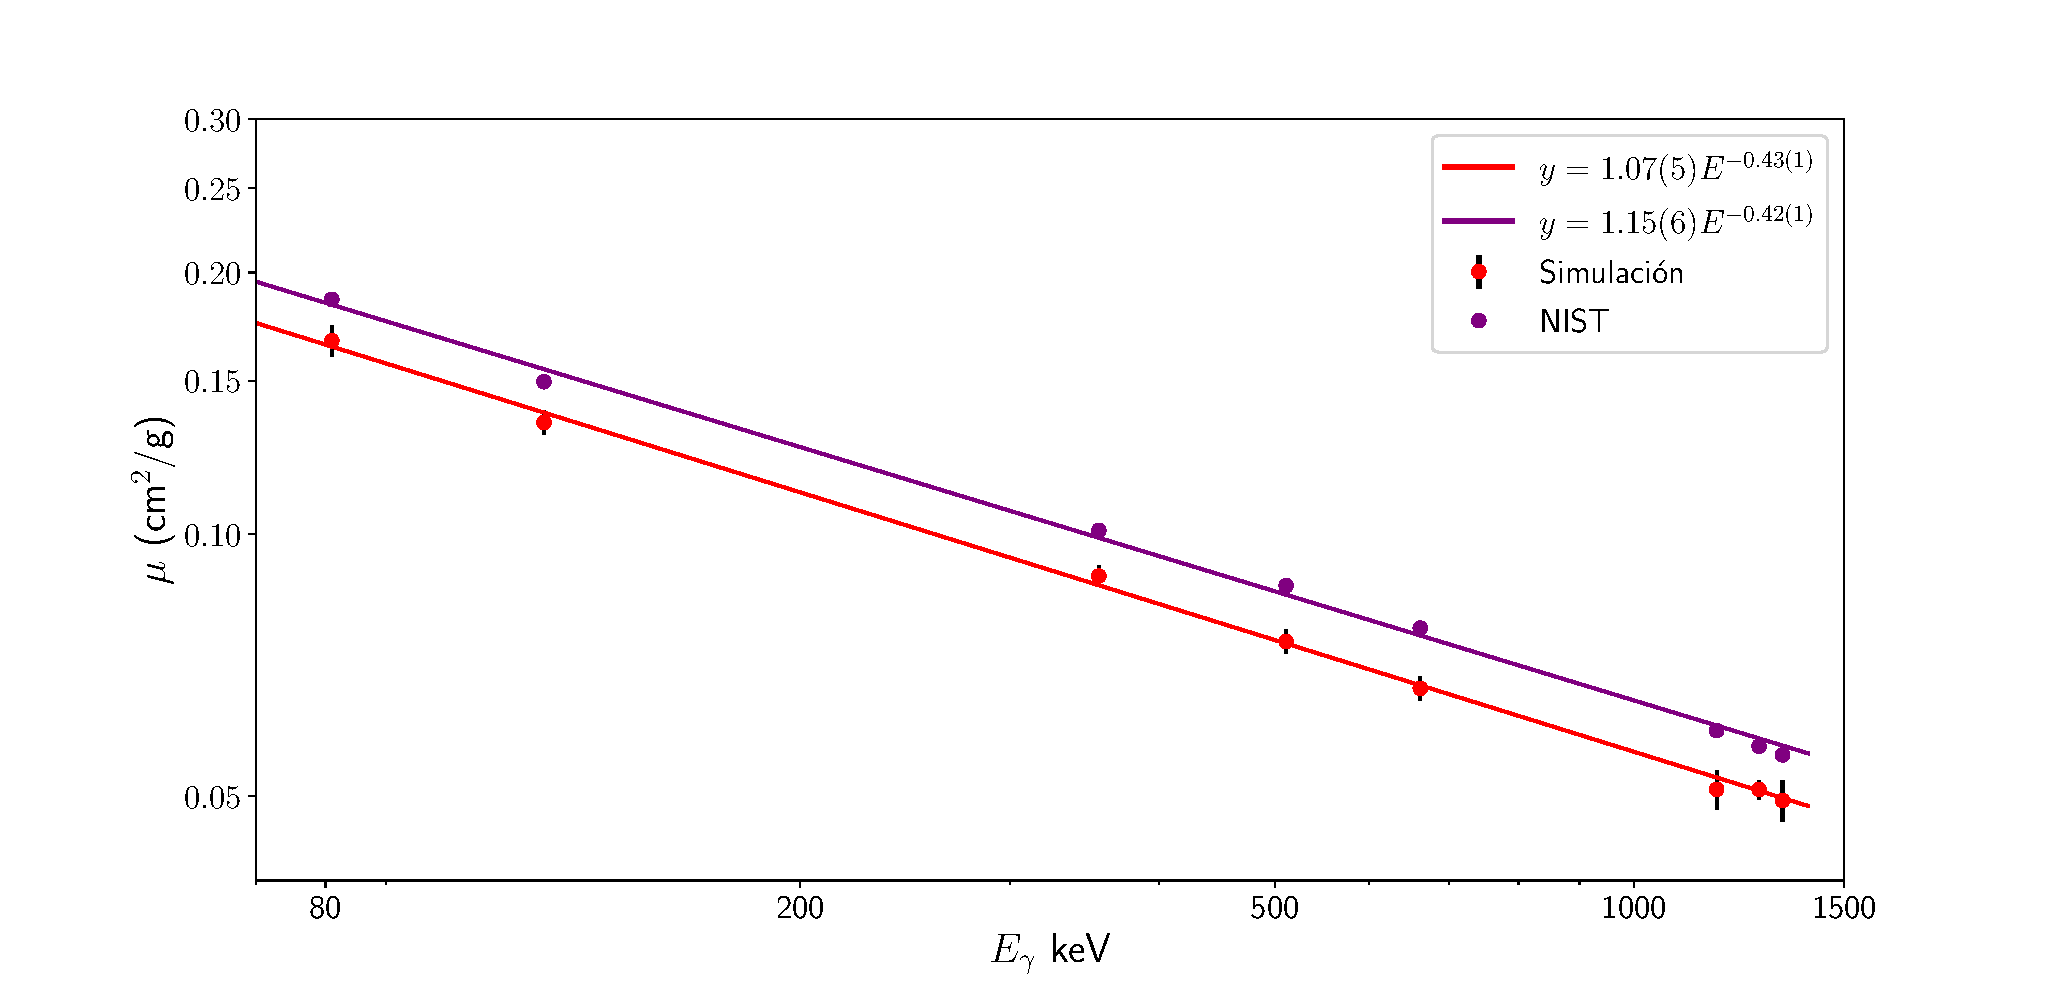
\includegraphics[width=1.0\linewidth]{Kap4/mu-trans-m4.pdf}
	\caption{Ajuste para encontrar $\alpha$ y $n$ a partir de los diferentes $\mu$/$\rho$. Morteros4.}
	\label{fig:mu-trans-m4}
\end{figure}
 
 
 \subsection{Retrodispersión.}
 
 \begin{figure}[H]
 	\centering
 	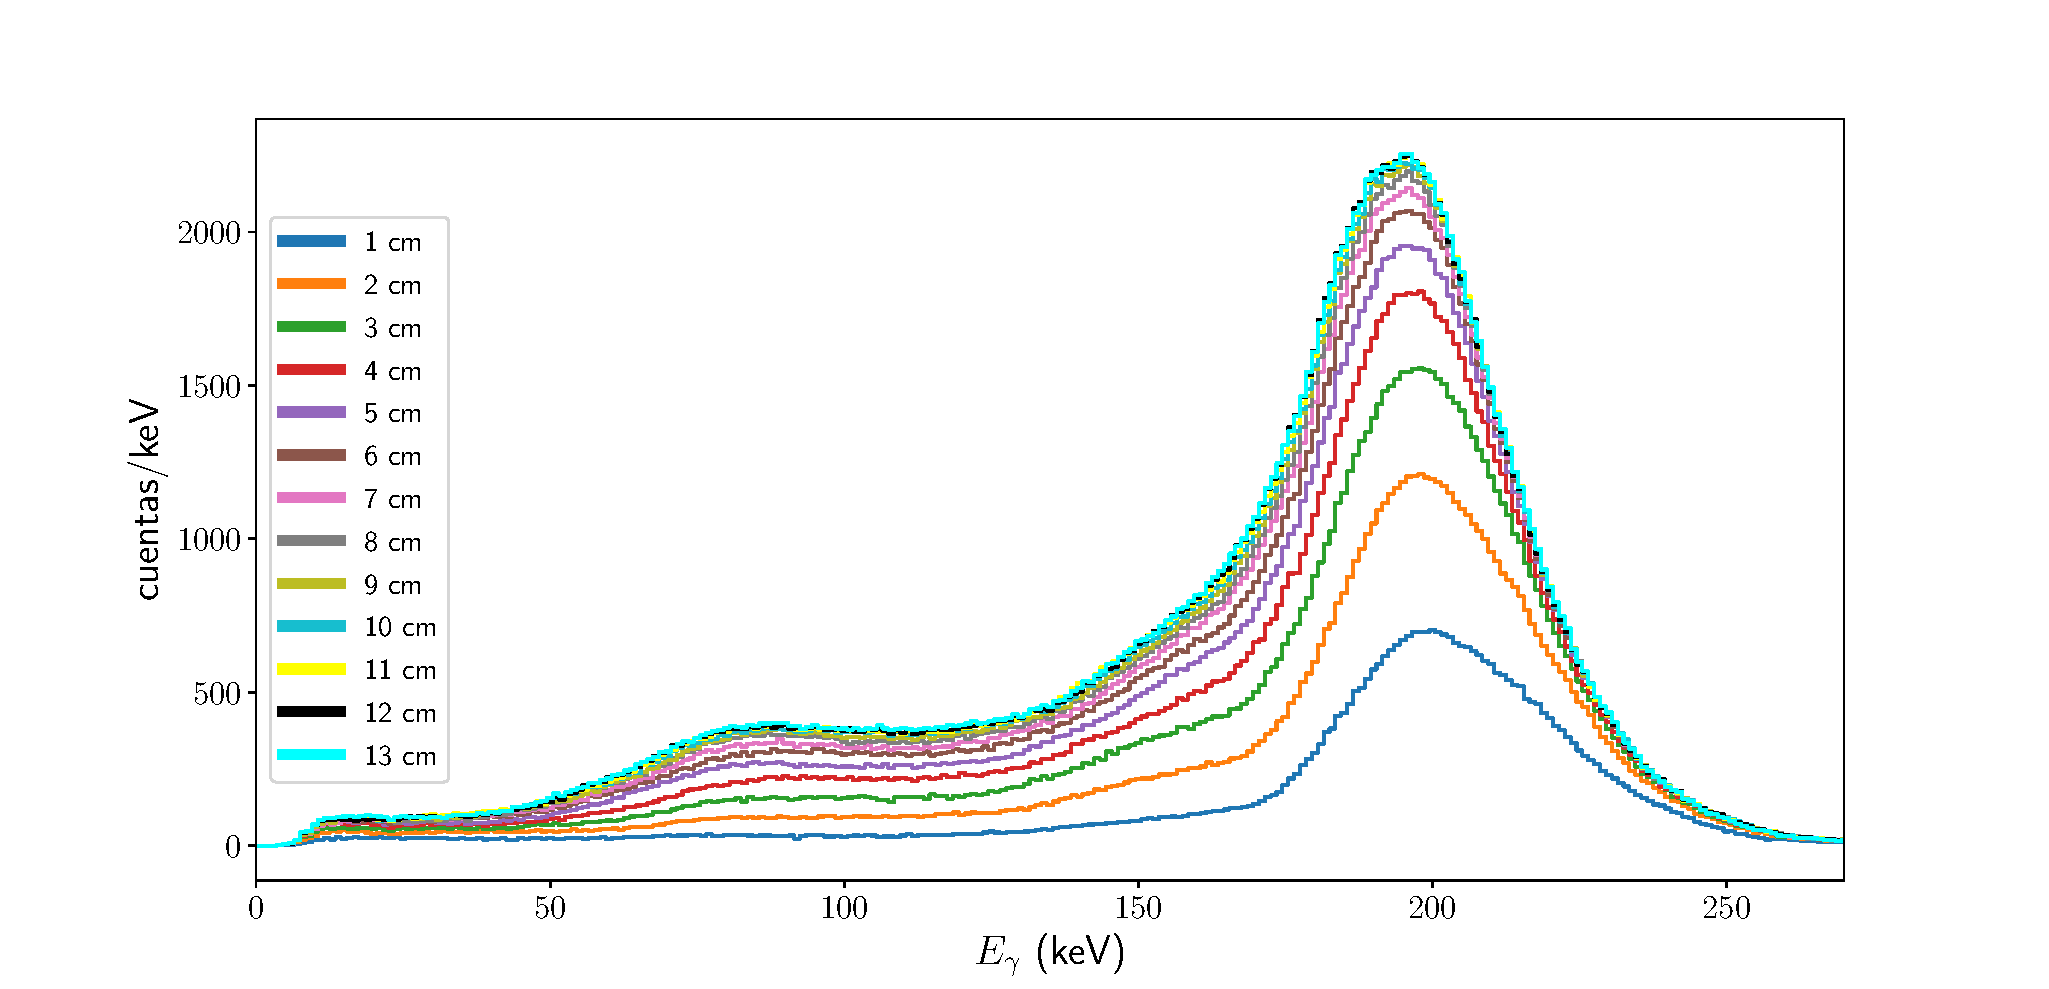
\includegraphics[width=1.0\linewidth]{Kap4/espectro_m4.pdf}
 	\caption{Espectro de 10 láminas de Morteros4.}
 	\label{fig:espectrom4}
 \end{figure}
 
 \begin{figure}[H]
 	\centering
 	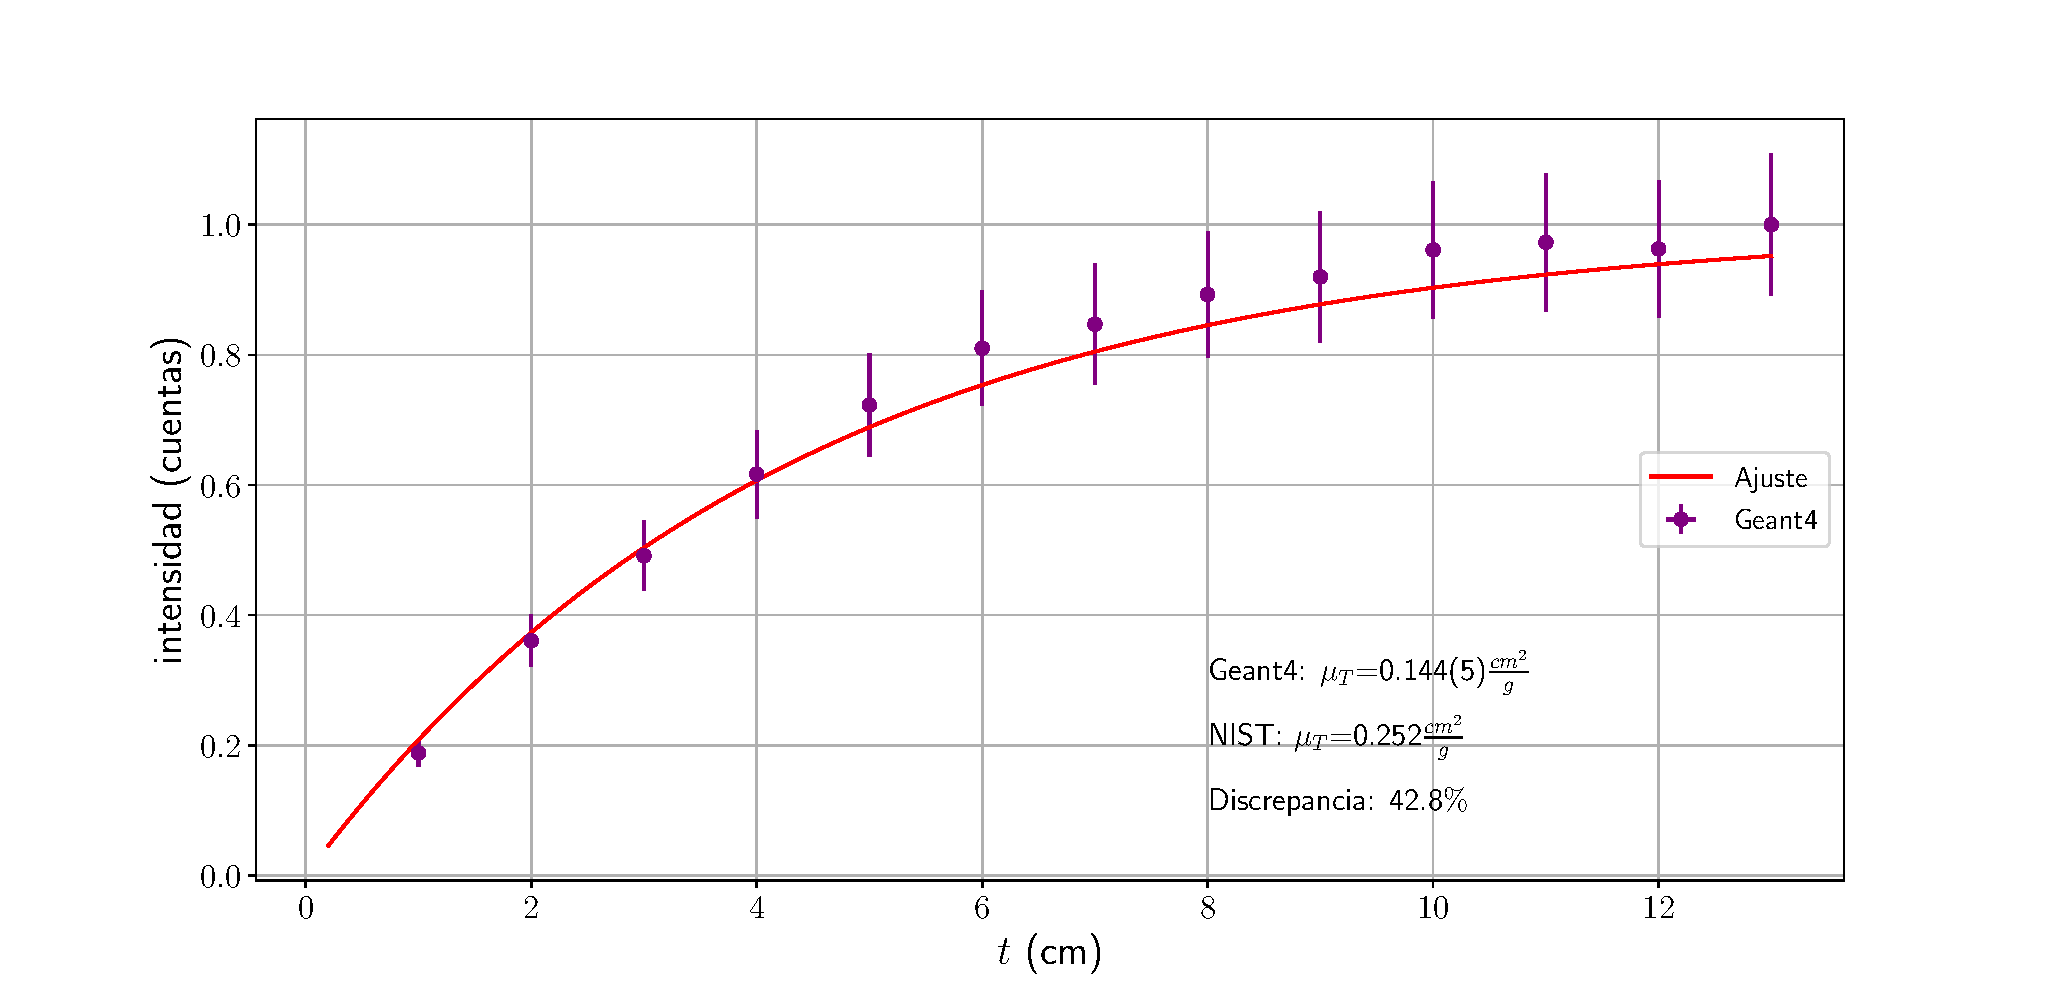
\includegraphics[width=1.0\linewidth]{Kap4/mu_T-m4.pdf}
 	\caption{valores de $\mu_T$. Morteros4.}
 	\label{fig:mut-m4}
 \end{figure}
 
 
 
 
 \section{Morteros 5.}
 
    \begin{table}[H]
 	\centering
 	\begin{tabular}{|c|c|c|c|c|c|c|c|}
 		\hline
 		\multicolumn{8}{|c|}{Laminas de Morteros5}                                                                             \\ \hline
 		\multirow{2}{*}{Lamina \#} & Masa {[}g{]} & H1 {[}cm{]} & H2 {[}cm{]} & L1 {[}cm{]} & L2 {[}cm{]} & W1 {[}cm{]} & W2 {[}cm{]} \\ \cline{2-8} 
 		& (+/- 0.01)   & \multicolumn{6}{c|}{(+/- 0.001)}                                                  \\ \hline 		1                          & 136.58       & 9.762          & 9.734      & 96.67         & 96.10       & 1.009       & 0.877       \\ \hline
 		2                          & 133.28       & 9.660          & 9.646      & 96.00         & 96.42       & 0.850       & 0.887       \\ \hline
 		3                          & 128.12       & 9.629          & 9.673      & 95.11         & 95.30       & 0.927       & 0.824       \\ \hline
 		4                          & 130.35       & 9.670          & 9.677      & 95.77         & 96.93       & 0.869       & 0.912       \\ \hline
 	\end{tabular}
 	\caption{Medidas experimentales del lote morteros5.}
 	\label{t:medidas-morteros5}
 \end{table}
 
 
 \begin{table}[H]
 	\centering
 	\begin{tabular}{|c|c|c|}
 		\hline
 		\multirow{2}{*}{Material} & \multicolumn{2}{c|}{4 placas} \\ \cline{2-3}
 		& g         	& \%        	\\ \hline
 		Cemento Portland      	& 600      	& 75    	\\ \hline
 		Arena Sílice         	& 0      	& 0    	\\ \hline
 		Agua                  	& 200     	& 25     	\\ \hline
 	\end{tabular}
 	\caption{Proporción porcentual en la elaboración de morteros4.}
 	\label{t:materiales-morteros5}
 \end{table}
 
 \begin{equation} \label{densidad-mor5}
 \rho=\frac{masa}{volumen}=1.60(6) g/cm^3
 \end{equation}
 
 
 \subsection{Transmisión.}
 
\begin{figure}[H]
	\centering
	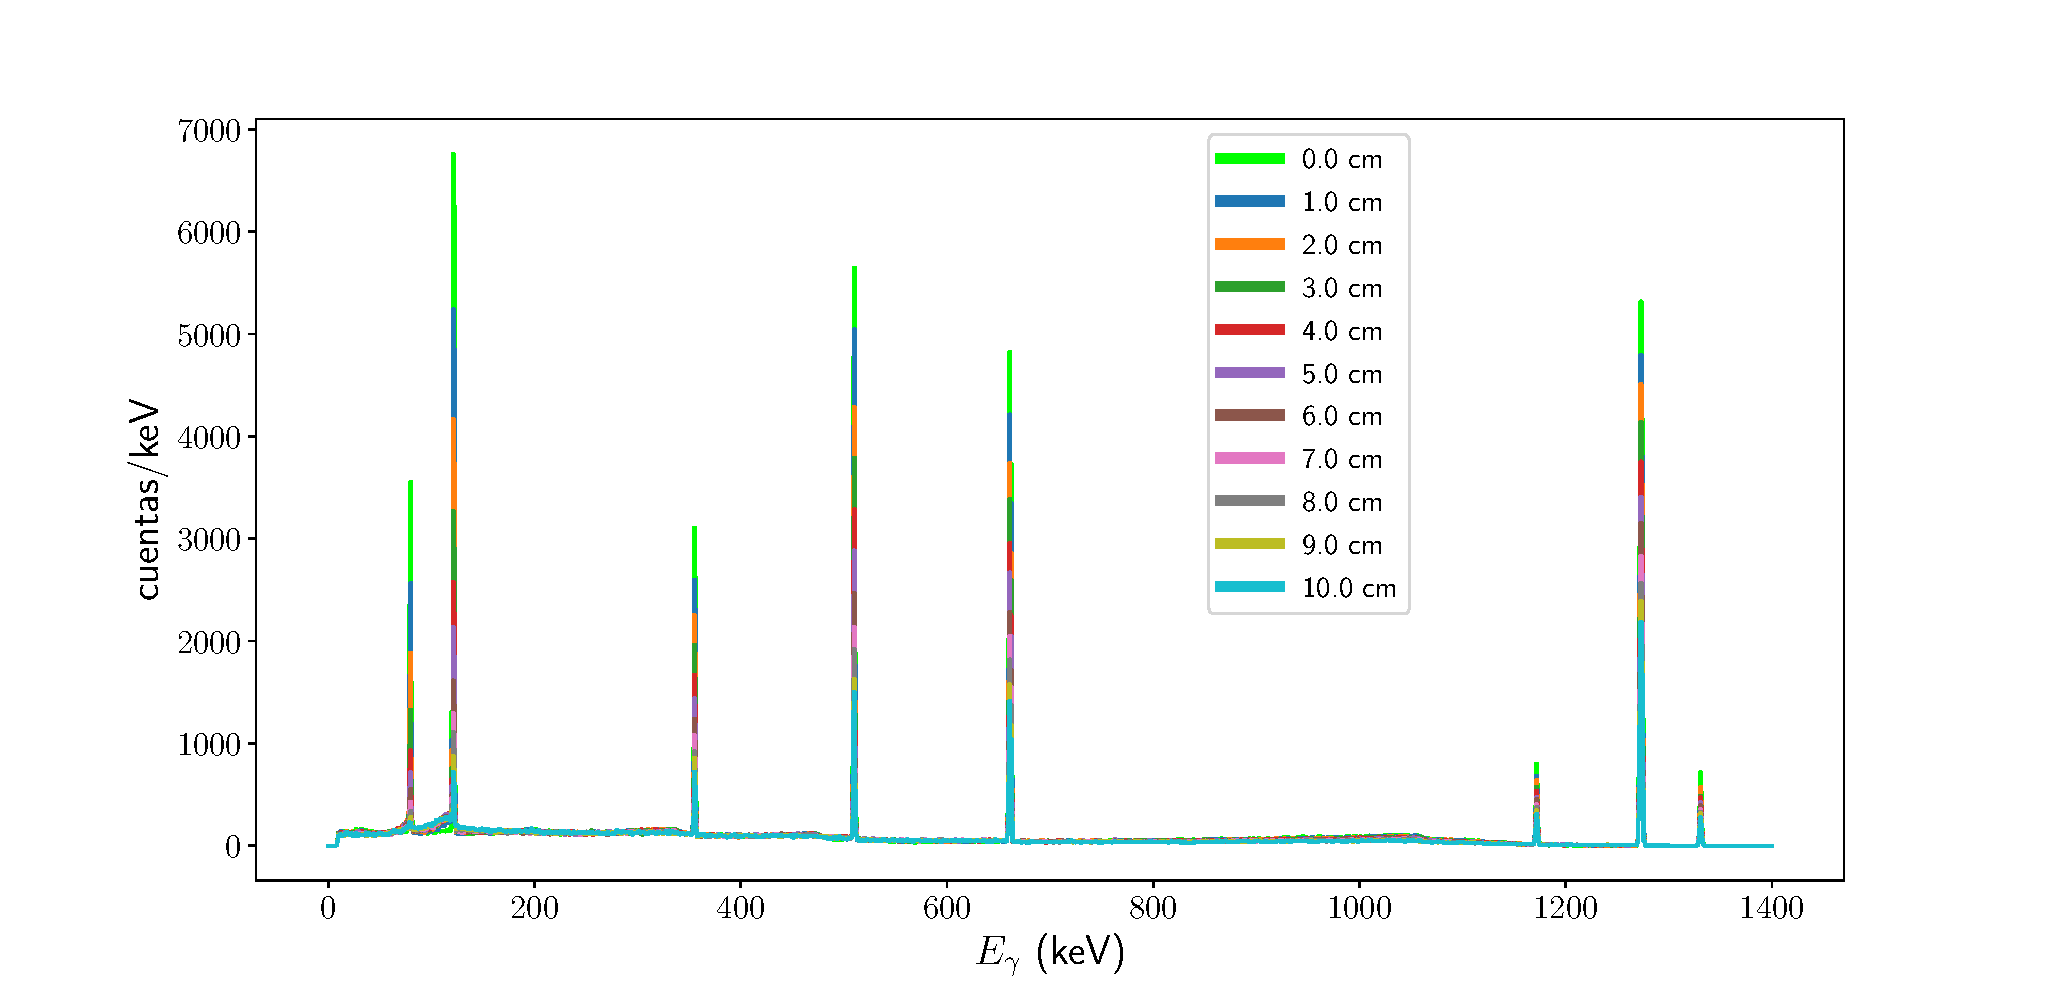
\includegraphics[width=1.0\linewidth]{Kap4/espectro_m5-10Mtrans.pdf}
	\caption{Espectro de 10 láminas de Morteros5. Transmisión}
	\label{fig:espectrom5-10mtrans}
\end{figure}
 
\begin{figure}[H]
	\centering
	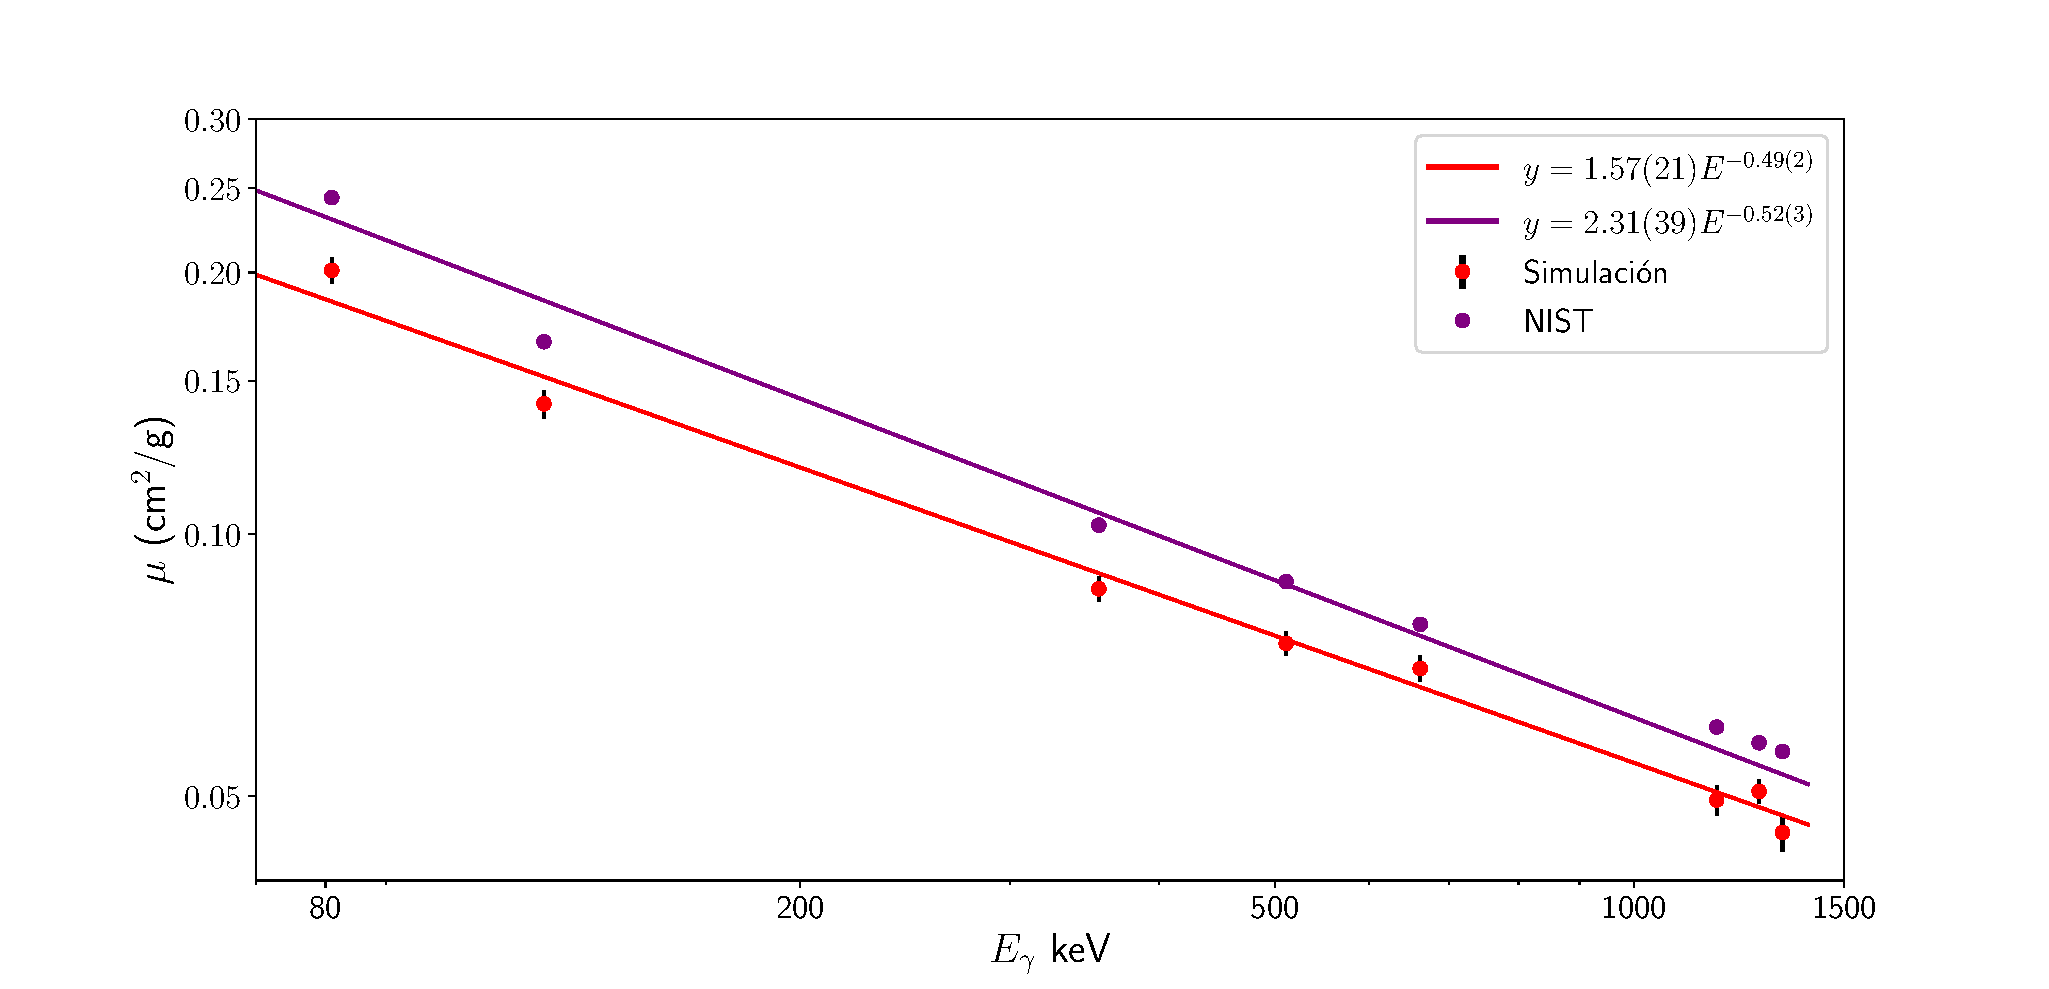
\includegraphics[width=1.0\linewidth]{Kap4/mu-trans-m5.pdf}
	\caption{Ajuste para encontrar $\alpha$ y $n$ a partir de los diferentes $\mu$/$\rho$. Morteros5.}
	\label{fig:mu-trans-m5}
\end{figure}
 
 \subsection{Retrodispersión.}
 
\begin{figure}[H]
	\centering
	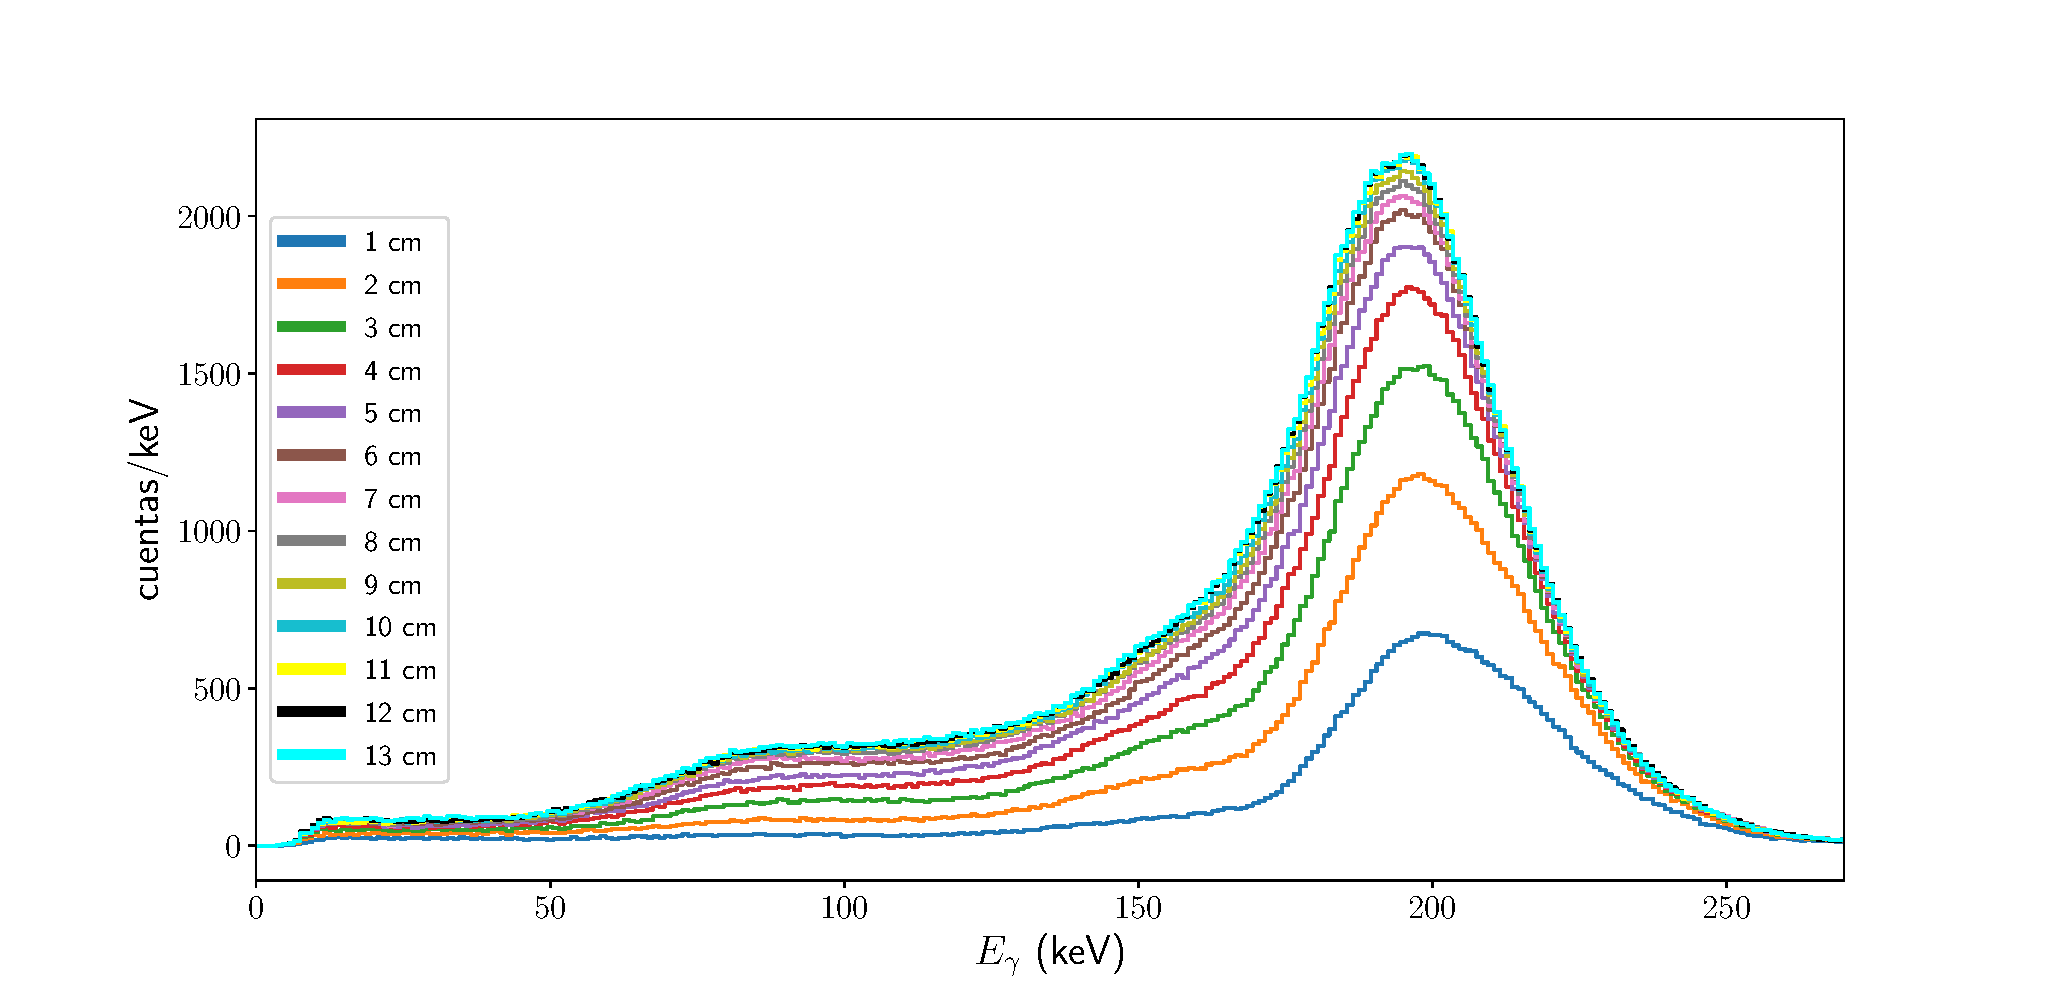
\includegraphics[width=1.0\linewidth]{Kap4/espectro_m5.pdf}
	\caption{Espectro de 10 láminas de Morteros5.}
	\label{fig:espectrom5}
\end{figure}

\begin{figure}[H]
	\centering
	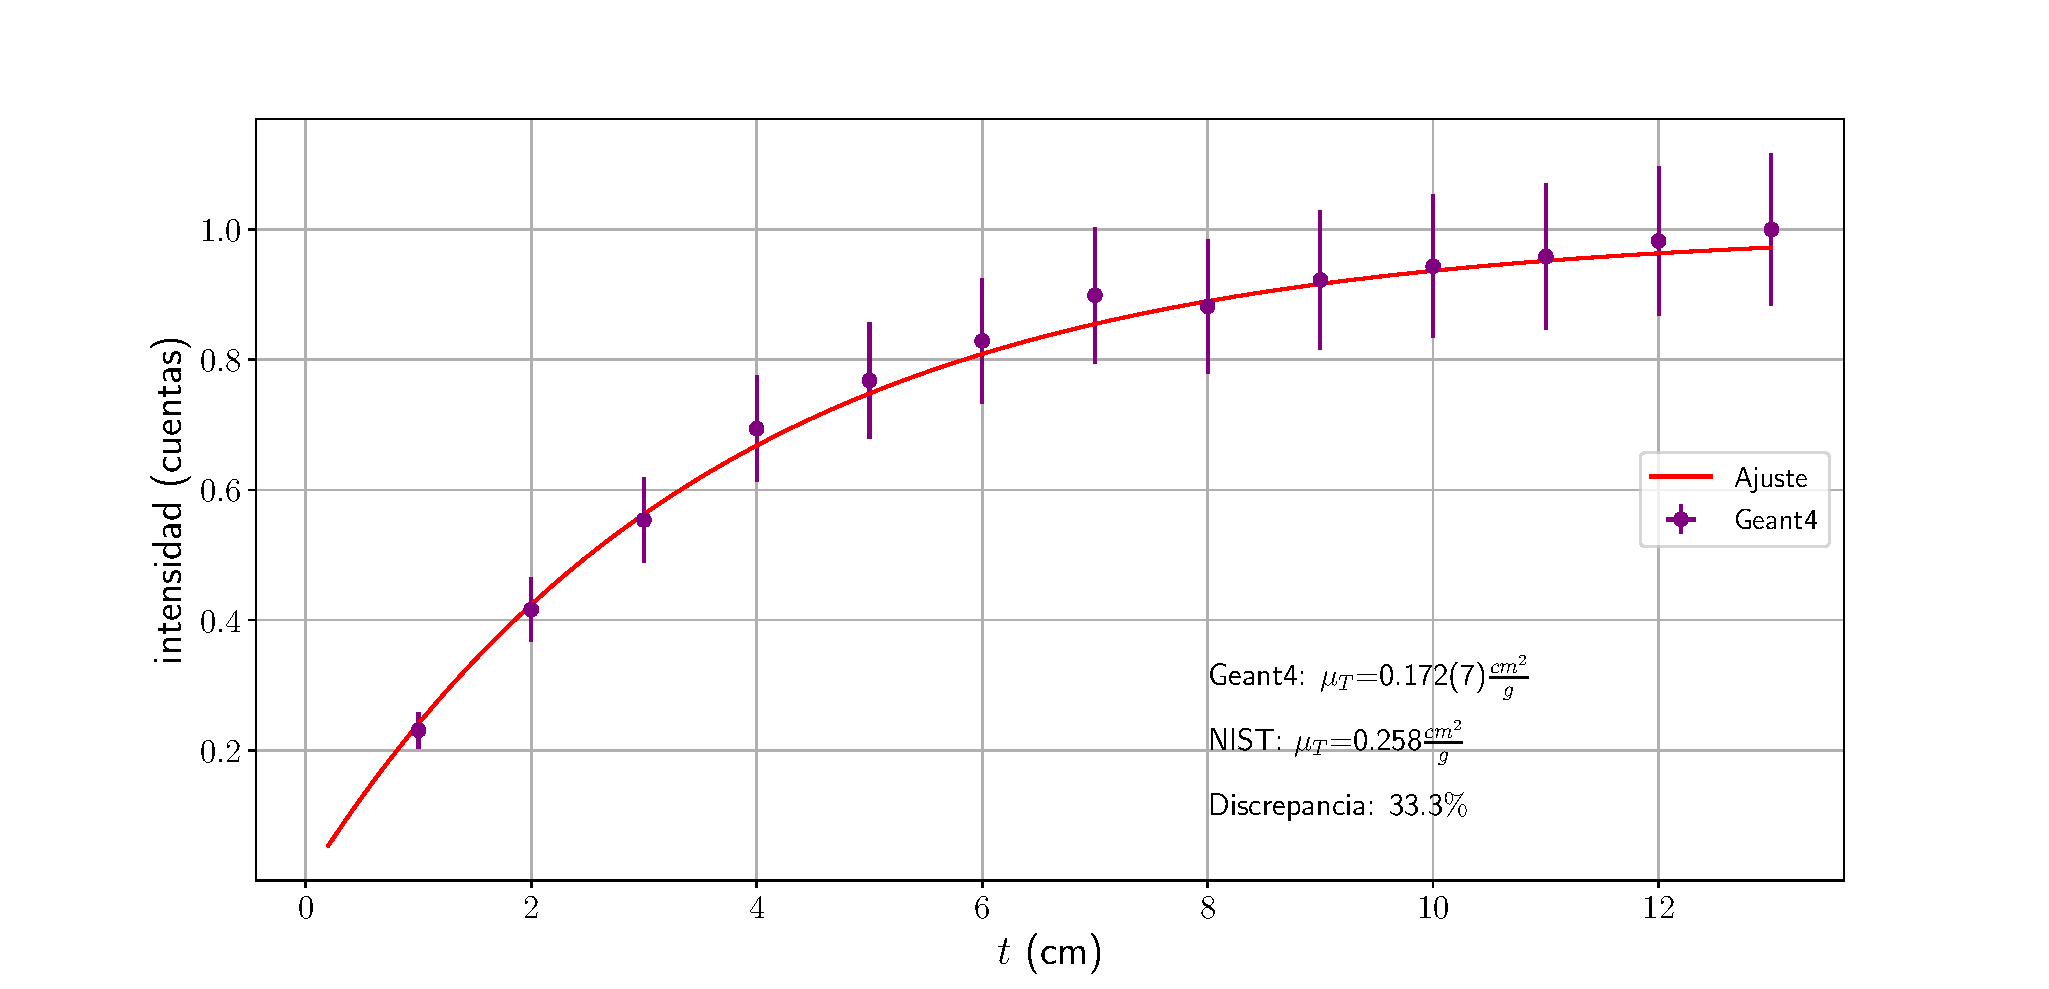
\includegraphics[width=1.0\linewidth]{Kap4/mu_T-m5.pdf}
	\caption{Valores de $\mu_T$. Morteros5.}
	\label{fig:mut-m5}
\end{figure}
\chapter{Cap\'{\i}tulo ...}
Se deben incluir tantos cap\'{\i}tulos como se requieran; sin embargo, se recomienda que la tesis  o trabajo de investigaci\'{o}n tenga un m\'{\i}nimo 3 cap\'{\i}tulos y m\'{a}ximo de 6 cap\'{\i}tulos (incluyendo las conclusiones).\\
\chapter{Comparación entre simulación y experimento.}
\begin{appendix}
\chapter{Anexo: Nombrar el anexo A de acuerdo con su contenido}\label{AnexoA}
Los Anexos son documentos o elementos que complementan el cuerpo de la tesis o trabajo de investigaci\'{o}n y que se relacionan, directa o indirectamente, con la investigaci\'{o}n, tales como acetatos, cd, normas, etc.\\

\chapter{Anexo: Nombrar el anexo B de acuerdo con su contenido}
A final del documento es opcional incluir \'{\i}ndices o glosarios. \'{E}stos son listas detalladas y especializadas de los t\'{e}rminos, nombres, autores, temas, etc., que aparecen en el mismo. Sirven para facilitar su localizaci\'{o}n en el texto. Los \'{\i}ndices pueden ser alfab\'{e}ticos, cronol\'{o}gicos, num\'{e}ricos, anal\'{\i}ticos, entre otros. Luego de cada palabra, t\'{e}rmino, etc., se pone coma y el n\'{u}mero de la p\'{a}gina donde aparece esta informaci\'{o}n.\\

\chapter{Anexo: Nombrar el anexo C de acuerdo con su contenido}
MANEJO DE LA BIBLIOGRAF\'{I}A: la bibliograf\'{\i}a es la relaci\'{o}n de las fuentes documentales consultadas por el investigador para sustentar sus trabajos. Su inclusi\'{o}n es obligatoria en todo trabajo de investigaci\'{o}n. Cada referencia bibliogr\'{a}fica se inicia contra el margen izquierdo.\\

La NTC 5613 establece los requisitos para la presentaci\'{o}n de referencias bibliogr\'{a}ficas citas y notas de pie de p\'{a}gina. Sin embargo, se tiene la libertad de usar cualquier norma bibliogr\'{a}fica de acuerdo con lo acostumbrado por cada disciplina del conocimiento. En esta medida es necesario que la norma seleccionada se aplique con rigurosidad.\\

Es necesario tener en cuenta que la norma ISO 690:1987 (en Espa\~{n}a, UNE 50-104-94) es el marco internacional que da las pautas m\'{\i}nimas para las citas bibliogr\'{a}ficas de documentos impresos y publicados. A continuaci\'{o}n se lista algunas instituciones que brindan par\'{a}metros para el manejo de las referencias bibliogr\'{a}ficas:\\

\begin{center}
\centering%
\begin{tabular}{|p {7.5 cm}|p {7.5 cm}|}\hline
\arr{Instituci\'{o}n}&Disciplina de aplicaci\'{o}n\\\hline%
Modern Language Association (MLA)&Literatura, artes y humanidades\\\hline%
American Psychological Association (APA)&Ambito de la salud (psicolog\'{\i}a, medicina) y en general en todas las ciencias sociales\\\hline
Universidad de Chicago/Turabian &Periodismo, historia y humanidades.\\\hline
AMA (Asociaci\'{o}n M\'{e}dica de los Estados Unidos)&Ambito de la salud (psicolog\'{\i}a, medicina)\\\hline
Vancouver &Todas las disciplinas\\\hline
Council of Science Editors (CSE)&En la actualidad abarca diversas ciencias\\\hline
National Library of Medicine (NLM) (Biblioteca Nacional de Medicina)&En el \'{a}mbito m\'{e}dico y, por extensi\'{o}n, en ciencias.\\\hline
Harvard System of Referencing Guide &Todas las disciplinas\\\hline
JabRef y KBibTeX &Todas las disciplinas\\\hline
\end{tabular}
\end{center}

Para incluir las referencias dentro del texto y realizar lista de la bibliograf\'{\i}a en la respectiva secci\'{o}n, puede utilizar las herramientas que Latex suministra o, revisar el instructivo desarrollado por el Sistema de Bibliotecas de la Universidad Nacional de Colombia\footnote{Ver: www.sinab.unal.edu.co}, disponible en la secci\'{o}n "Servicios", opci\'{o}n "Tr\'{a}mites" y enlace "Entrega de tesis".

\end{appendix}
\addcontentsline{toc}{chapter}{\numberline{}Bibliograf\'{\i}a}
\bibliographystyle{apalike}
\bibliography{BibliMSc}
\end{document}